\documentclass{zbc-report}

\usetikzlibrary{shapes.geometric}  % Including shapes.geometric for TikZ
\usepackage[normalem]{ulem}
\useunder{\uline}{\ul}{}

%% Set up the bibliography
\usepackage{biblatex}
\addbibresource{report.bib}

%% Additional packages and commands
\usepackage{parskip}
\setlist{itemsep=-2pt} % Reducing white space in lists slightly
\renewcommand{\deg}{\si{\degree}\xspace} % Use \deg easily, everywhere

%% Set up the minted package
\usepackage[cachedir=_minted-report]{minted}
\setminted{
    linenos=true,
    breaklines=true,
    fontsize=\footnotesize,
    frame=lines,
    framesep=2mm,
    baselinestretch=1.2,
    bgcolor=gray!10,
    style=vs,
    mathescape=true,
}

%% ----------------------------------------------------------------------
%%    Begin of document + Frontmatter (Roman page numbering)
%% ----------------------------------------------------------------------

\begin{document}

\frontmatter

%% Define the main parameters
\title{Semesterproject Webshop}
\subtitle{Computer Science\\ 2nd Semester}
\author{Carsten Lydeking}

\subject{Software Design and Construction} % Cover only
\large\affiliation{Zealand Business College} % Cover only
\coverimage{figures/template-figures/binary.jpg} % Aspect ratio of 2:3 (portrait) recommended
\definecolor{title}{HTML}{4884d6} % Color for cover title

\makecover

\begin{titlepage}

\begin{center}

%% Print the title
{\makeatletter
\largetitlestyle\fontsize{45}{45}\selectfont\@title
\makeatother}

%% Print the subtitle
{\makeatletter
\ifdefvoid{\@subtitle}{}{\bigskip\titlestyle\fontsize{20}{20}\selectfont\@subtitle}
\makeatother}

\bigskip
\bigskip

%% Print the name of the author
{\makeatletter
\largetitlestyle\fontsize{25}{25}\selectfont\@author
\makeatother}

\bigskip
\bigskip

%% Print table with names and student numbers
\setlength\extrarowheight{2pt}
\begin{tabular}{c}
    cal002@edu.zealand.dk \\
\end{tabular}

\vfill

%% Print some more information at the bottom
\begin{tabular}{l r}
    Lecturer, SWC:    & Henrik Kryger Høltzer\\
    Lecturer, SWD:    & Mikkel Lynggaard Krarup\\
    Project Deadline: & \ddmmyydate{30/05/24} \\
    Handed-in:       & \ddmmyydate{\today} \\
    Faculty:         & Computer Science \\
    Semester:        & 2nd Semester \\
    Word Count:      & 48180 Characters (including spaces) \\
\end{tabular}

\bigskip
%% Add a source and description for the cover and optional attribution for the template
\begin{tabular}{l r}
    Cover: & Generated image of binary using DALL-E \\
    Style: & ZBC template -- created by Carsten Lydeking \\
\end{tabular}


%% Insert the Zealand logo at the bottom of the page
\begin{tikzpicture}[remember picture]
    \node[above=10mm] at (current page.south) {%
        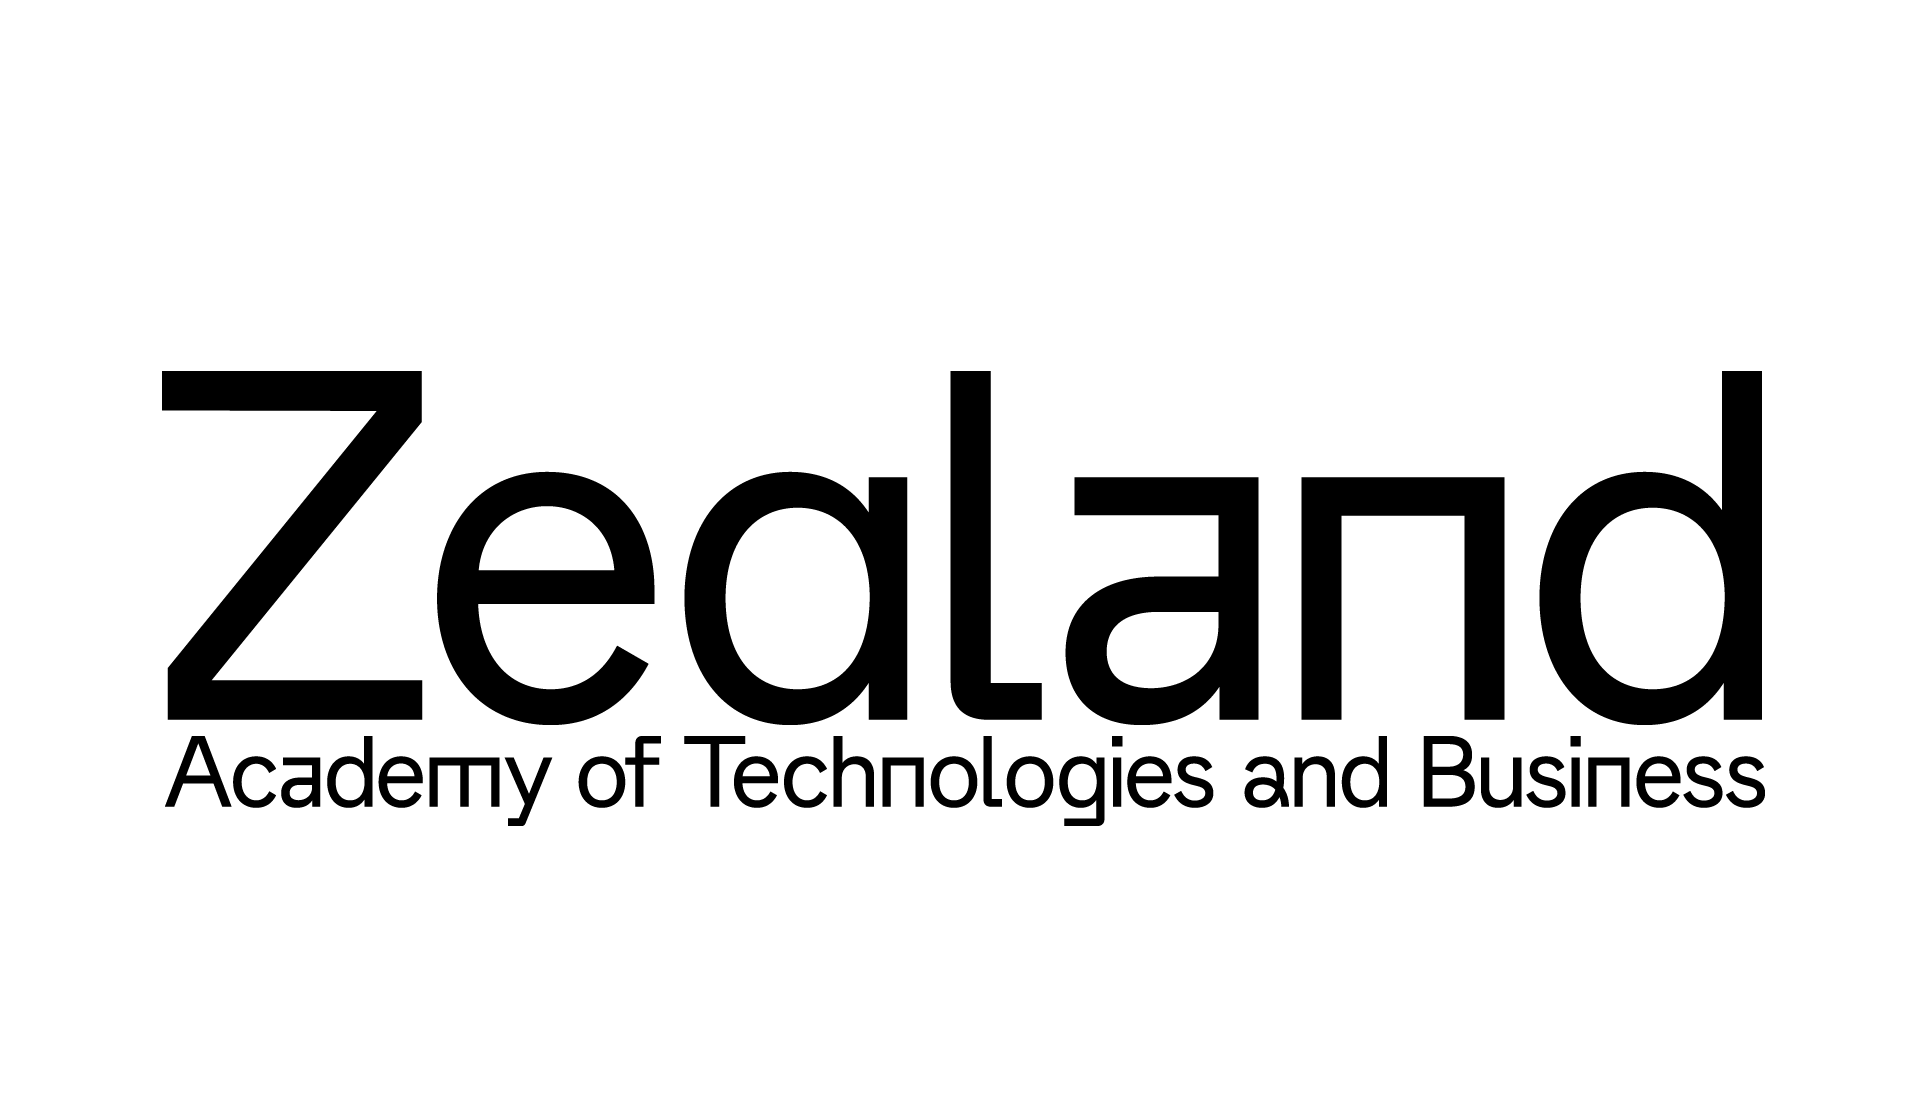
\includegraphics[width=0.35\textwidth]{figures/template-figures/zealandcombinedlogo}
    };
\end{tikzpicture}

\end{center}

\end{titlepage}

\tableofcontents
\listoffigures
\listoftables

\chapter*{Nomenclature}
\addcontentsline{toc}{chapter}{Nomenclature}

\section{Abbreviations and definitions}
\label{sec:abbreviations}
The following abbreviations and definitions are used throughout the report:

\renewcommand{\arraystretch}{2}
\begin{longtable}{l p{13.5cm}}
    \textbf{Abb.}  & \textbf{Definition}  \\ \hline
        DB           & Database: A structured collection of data stored electronically. \\ \hline
        RDB          & Relational Database: A type of DB that stores and provides access to data points that are related to one another. \\ \hline
        DBMS         & Database Management System: Software that handles the storage, retrieval, and updating of data in a database. \\ \hline
        RDBMS        & Relational DBMS: A database management system based on the relational model introduced by E.F. Codd. \\ \hline
        SQL          & Structured Query Language: A programming language used to manage and manipulate relational databases. \\ \hline
        CRUD         & Create, Read, Update, Delete The four basic operations of persistent storage: adding, retrieving, modifying, and removing data. \\ \hline
        GUI          & Graphical User Interface  A user interface that allows users to interact with electronic devices using graphical icons and visual indicators. \\ \hline
        PK           & Primary Key:A unique identifier for each record in a database table. \\ \hline
        FK           & Foreign Key: A field in a database table that links to the primary key of another table. \\ \hline
        NML          & Normalization: In relation to RDB design, the process of organizing the columns (attributes) and tables (relations) to minimize data redundancy. \\ \hline
        1NF          & First Normal Form: A stage of NML where each table has atomic (i.e. indivisible) values and each record needs to be unique. \\ \hline
        2NF          & Second Normal Form: A stage of NML where it meets all the requirements of the 1NF and does not have partial dependency. \\ \hline
        3NF          & Third Normal Form: A stage of NML where it meets all the requirements of the 2NF and has no transitive functional dependencies. \\ \hline
        ERD          & Entity Relationship Diagram: A graphical representation of entities and their relationships to each other, typically used in database design. \\ \hline
        UML          & Unified Modeling Language: A standardized modeling language used to specify, visualize, construct, and document the artifacts of software systems. \\ \hline
        DDL          & Data Definition Language: A subset of SQL used to define database structures, such as tables, schemas, and databases. \\ \hline
        DML          & Data Manipulation Language: A subset of SQL used for adding (inserting), deleting, and modifying (updating) data in a database. \\ \hline
        DCL          & Data Control Language: A subset of SQL used to control access to data in a database. \\ \hline
        TCL          & Transaction Control Language: A subset of SQL used to manage the changes made by DML statements. \\ \hline
        XML          & Extensible Markup Language: A markup language that defines a set of rules for encoding documents in a format that is both human-readable and machine-readable. \\ \hline
        JSON         & JavaScript Object Notation: A lightweight data-interchange format that is easy for humans to read and write, and for machines to parse and generate. \\ \hline
    \renewcommand{\arraystretch}{1}
\end{longtable}

%% ----------------------------------------------------------------------
%%    Mainmatter (Arabic page numbering)
%% ----------------------------------------------------------------------

\mainmatter

\chapter{Introduction}
\label{chapter:introduction}

\section{Case}
Blomsterbinderiet er en mindre butik, der ønsker en hjemmeside til at kunne servicere kunder online.
Deres produkt er primært blomsterdekorationer til forskellige begivenheder og af varierende størrelse.
Blomsterbinderiet har både walk-ins, bestillinger og et samarbejde med flere bedemænd i Roskilde og omegn. Til bedemænd er der særlige services, bl.a. levering til begravelser. Bestillinger fra private skal afhentes.
Selve butikken er fysisk placeret som en afdeling i Meny Roskilde og har ansat 3 blomsterdekoratører og et varierende (3-10) antal ufaglærte, hovedsageligt unge, assistenter.
Betalinger sker via MobilePay for private og via faktura for erhverv. Dette passer butikken godt, da de ofte gerne vil kunne kontakte kunden med spørgsmål, inden de acceptere ordren.
Ingen i butikken har IT erfaring og der er ikke budget til at have en fast IT supporter. Butiksbestyren, som vil være aftager af vores software, har talt om følgende:
\begin{itemize}
	\item Hjemmeside, hvor kunder kan afgive bestillinger
	\item Mulighed for at afvise bestillinger/slå bestillinger fra
	\item Mulighed for at kontakte kunden inden de acceptere en afgivet ordre
	\item Mulighed for et galleri til at inspirere kunderne
	\item Funktion hvor de kan se indkommende ordre evt notifiktaion
	\item Funktion hvor kunder kan kontakte butikken (evt. kontaktformular)
	\item Særlige funktionaliteter til bedemænd
	\item Kunden skal kunne vælge mellem forskellige størrelser af samme produkt
	\item Funktion, så de selv kan oprette, opdatere og arkivere produkter
	\item Mulighed for at få salgsstatestik, af endnu uspecificeret karatker.
	\label{list:butikkens-ønsker}
\end{itemize}

\section{Projektet}

\subsection{Problemformulering}
Hvordan kan man gennem Razor Pages, Entity Framework og med SCRUM som projektstyringsværktøj, udvikle en online webshop til BlomsterBinderiet, 
så den både imødekommer behovene hos almindelige kunder og lokale bedemænd gennem tilpassede brugeroplevelser og administrationsfunktioner.

\subsection{Formål}
Formålet med projektet er at udvikle en webshop til Blomsterbinderiet, der kan imødekomme behovene hos både almindelige kunder og lokale bedemænd. 
Dette skal ske gennem en brugervenlig og intuitiv brugergrænseflade, der giver kunderne mulighed for at afgive bestillinger, se produkter og kontakte butikken. 
Samtidig skal webshoppen give butikken mulighed for at administrere produkter, bestillinger og kunder, samt at se salgsstatistikker.

\subsection{Afgrænsning}
Projektet vil fokusere på udviklingen af en webshop til Blomsterbinderiet, der kan imødekomme behovene hos både almindelige kunder og lokale bedemænd. 
Der vil være mindre afvigelser fra hvad man ville gøre i virkeligheden, da projektet er et skoleprojekt og ikke et betalt kontraktprojekt. 
Dermed vil der være punkter, hvor fokus er på selve processen, dokumentation af denne og levere et produkt til skolastisk vurdering.

\subsection{Rapportens opbygning}
Rapporten vil begynde med projektets udgangspunkt og rammer i \Cref{chapter:udgangspunkt}, efterfulgt af en analyse af Blomsterbinderiets forretningsmodel i \Cref{chapter:forretningsanalyse}. 
Dette videreføres i \Cref{chapter:scrum} om SCRUM processen som projektstyringsværktøj og hvordan det anvendes i denne sammenhæng, bl.a. anvendelse af User Stories.
Herefter følger \Cref{chapter:software-design} om software design, der beskriver både den indledende analysen bag modeller og strukturer samt hvilke teknologier der tænkes er anvendt.
Dette vil føre over i \Cref{chapter:scrum-documentation} om selve udviklingen af projektet, hvor de enkelte Sprints dokumenteres. 
I \Cref{chapter:final-design} vil der være en gennemgang af projektets endelig implementering, beskrivelse og tankerne bag de vigtigste afvigelser fra den oprindelige plan.
Til sidst vil der i \Cref{chapter:conclusion} være en konklussion og perspektivering, der opsummerer projektet og dets resultater, samt giver et bud på hvordan et fremtidigt projekt kunne videreføres.
Bemærk, alle kapiteler opsummeres i \Cref{sec:conclusion_summary} med henblik på at give et samlet overblik over projektet, i stedet for at afrunde de individuelle kapitler med en opsummering. 
Tanken bag, er at give læseren en mulighed for at få et overblik over projektet, blot ved at læse \Cref{chapter:introduction} og derefter \Cref{chapter:conclusion}.

\subsection{Metode og teknologi}
Razor Pages (RP) er valgt, da det er pensum. 
Det giver dog nogle fordele bl.a. fordi det er en relativt simpel side-fokuseret model, der letter organisering og udviklingen af en webapplikation, der kræver flere særskilte sider, bl.a. til produkter, fremvise analyser m.m. 
Gennem Entity Framework (EF) kan vi bruge Code First approach, der letter vores udvikling, ved bl.a. at simplificere implementering af mindre modifikationer og speeder processen op, 
da vi kan fokusere på C-sharp klasserne som udgangspunkt for vores database modellering og styring. Hertil understøtter EF Language Integrated Query (LINQ), der muliggøre at kode typesikrede queries direkte i C-sharp. 
Det gør koden mere læsbar, vedligeholdelsesvenlig og vi skal heller ikke manuelt administrere SQL-scripts (samt det reducerer risikoen for SQL-injektionsangreb). 
Alt i alt, så forenkler det administrationen af applikationens datalag. En SQL-database giver et struktureret miljø til lagring af data, hvilket er essentielt for produktkataloget, brugerinformation og ordrestyring i projektet. 
Den strukturerede tilgang sikrer dataintegritet og letter komplekse forespørgsler, der fx anvendes ved analyser. Vi er bundet til SQL gennem EF.
GitHub anvendes til versionskontrol for at forenkle udviklingen. Det giver et effektivt miljø til versionskontrol og projektstyring, hvilket gør det til et solidt valg til næsten alle software projekter. 
Yderligere giver det mulighed for at branche og teste nye funktionaliteter men stadig have et minimum viable product på master branch. 
Visual Studio 2022 og ASP.NET Core Integration: Integrationen mellem Razor Pages, Entity Framework, GitHub og Visual Studio 2022 giver et kraftfuldt udviklingsmiljø til test og implementering af projektet. 
Denne integrerede tilgang forenkler udviklingsprocessen, fra skrivning af kode til administration af databaser og implementering af applikationen.
Simply.com er valgt som webhotel på baggrund af projektets scope, samt at de tilbyder forholdsvist lave udgifter til drift.

\chapter{Udgangspunkt for projektet}
\label{chapter:udgangspunkt}

Den 11. april blev det originale team splittet op. Dette kapitel anvendes til at reflektere over forløbet op til opsplitningen, hvad der skete undervejs og efterfølgende, samt de tilknyttede overvejelser.
Dette kapitel er altså ikke en beskrivelse af selve \emph{SCRUM}-processen, men et udgangspunkt for en ny opstart. Kapitlet danner derfor grundlag for en ny projektplan, der vil blive udarbejdet i de næste kapitler.

\section{Sprint Retrospektive}
For at holde \emph{SCRUM}-rammen, vil jeg bruge et \emph{Sprint retrospektive} til at reflektere over opsplitningen.
Jeg tillader mig dog at tilføje punktet "hvad var planen" til "Hvad gik godt, hvad gik skidt og hvad gør vi til næste gang". Grundet det reflekterende perspektiv, skrives afsnittet i datid.

\subsubsection{Hvad var planen}
Der blev med projektkontrakten sat en ramme for samarbejdet, og teamet har tidligere arbejdet sammen om semesterprojektet i første semester.
Der var en fælles, udtalt forståelse om et højt ambitionsniveau for projektet, og \emph{SCRUM} skulle være grundlaget for selve projektstyringen.
Arbejdsbyrden blev sat til at være indenfor normal undervisningstid på de gængse undervisningsdage (mandag-tirsdag og torsdag-fredag).

\subsubsection{Hvad gik godt}
Businessanalysen med bl.a. \emph{BMC} og \emph{SWOT} blev relativt hurtigt eksekveret.

\subsubsection{Hvad gik skidt}
Der var blandt alle medlemmer, en eller anden form for utilfredshed med de andre i teamet, dog ikke noget der blev luftet åbent. 
Der var tillige friktioner mellem visse teammedlemmer fra sidste projekt, som måske var begyndt i starten af studiet. Utilfredsheden samt friktionerne blev mere og mere tydelige og begyndte at påvirke samarbejdet. 
Eksempelvis blev det nævnt i en sidebemærkning, at det var frustrerende for et teammedlem, at den officielle frokostpause blev sprunget over, fordi et andet teammedlem ikke medbragte eller spiste frokost og derfor ønskede at gå tidligere hjem. 
Efter gruppedannelsen begyndte dele af teamet at forlange, at der kun måtte anvendes koncepter, syntax m.m. som var blevet undervist i eller havde været anvendt i opgaverne i semesteret. 
Der var bl.a. en situation, hvor et forslag om at anvende denormalisering af databasen, ikke engang blev taget op i plenum, før en fra teamet kom med en person-orienteret kommentar.
Friktionerne, den passive-aggressive tone m.m. resulterede i en form for mistillid, der skabte en dårlig stemning for alle teammedlemmer. 
Dette miljø nedbrød enhver konstruktiv dialog, og det førte til konklusionen, at et professionelt samarbejde ikke længere var en mulighed.

Derudover var der en meget forskellig opfattelse af, hvordan \emph{SCRUM} skulle anvendes. Der var teamets ønske, fra sidste projekt, om mere overordnet styring. Dette forsøgtes implementeret i dette projekt, da en \emph{SCRUM master} fremlagde en overordnet tidsplan for en dag, hvor det var nødvendigt, at hele teamet arbejdede sammen. 
Situationen udviklede sig desværre til en person-orienteret kommentar, hvor et teammedlem fortalte \emph{SCRUM master}, at denne skulle stoppe med at prøve på at være projektleder og bestemme over de andre teammedlemmer.

\subsubsection{Hvad gøres anderledes til næste gang}
Der kan spekuleres i, hvor mange af disse udfordringer, der kunne være blevet udglattet eller måske endda undgået, hvis den interpersonelle kemi i teamet havde været bedre. Jeg vil dog stadig nedfælde nogle punkter, der kan anvendes til fremtiden.

Et højt ambitionsniveau kan stå i kontrast til den begrænsede arbejdstid, som teamet fastsatte. Fremover bør der estimeres et mere konkret mål for et projekt og derefter afsættes tid eller vice versa, hvis ønsket om at holde studiet indenfor undervisningstiden vægtes højest.

Den overordnede ramme, i dette tilfælde \emph{SCRUM}, bør også defineres mere klart. 
Selvom \emph{SCRUM} var forsøgt defineret i dette projekt, bl.a. var det beskrevet, at \emph{SCRUM master} skulle facilitere møderne, var der uenighed om, hvad det at \emph{facilitere} indebar. 
Hvis man vælger at have en \emph{SCRUM master}, så bør der være en klar relation mellem ansvar, pligter og beføjelser. 
Hvis \emph{SCRUM master} skal være \emph{process owner}, bør der være klarhed om, at \emph{SCRUM master} bl.a. kan, bør og skal indkalde til møder og sætte dagsorden samt tidsplan for disse. Selv i velfungerende og sammenrystede teams, sammensat af højt motiverede og kompetente medlemmer, er der behov for en med det overordnede ansvar for processen. 
Både teori og erfaring peger mod, at nye, uprøvede teams \cite{mit-newteams} kræver bl.a. klare mål og mere struktur for at lykkes og trives. Dette er yderligere understreget, når de individuelle medlemmer har begrænset erfaring indenfor feltet, de skal arbejde i.

\section{Videreførsel}
Dette afsnit er skrevet kort efter opsplitningen med henblik på at fremstille tanker og planlægning, der er foregået efterfølgende.

\subsection{Opdeling af arv}
Det materiale, der var udarbejdet i fællesskab, er fælles eje, og store dele af det vil gå igen uden citat, bl.a. forretningsanalyse. Andre dele vil dog være markant omskrevet, således at de følger tråden i dette projekt. Rapporten, som den så ud 11. april, er vedlagt som bilag og kan blive refereret ved behov i denne rapport.

\subsection{SCRUM som enkeltmand}
Det kan anskues som kunstigt at skulle videreføre \emph{SCRUM} med alt, hvad det indeholder, når man ikke har en \emph{Product Owner} og er et team bestående af én. Visse \emph{SCRUM}-artefakter kan dog anvendes til projektstyring, bl.a. \emph{User Stories} og \emph{Burndown Charts} bevare sit oprindelige formål. Det vil undersøges, hvorvidt en lektor kan indgå som \emph{Product Owner} til nogle sessioner.

\subsection{Sprint planning}
Tidsrammen fra opsplitningen til deadline giver knap syv uger til at komme i mål. 
Det forventes, at der afsættes en uge til at sammenfatte og redigere eksisterende materiale, bl.a. omskrive og reestimere \emph{User Stories}. Dette vil blive kaldt \emph{Sprint 0}.
Den resterende tid deles op i fem \emph{Sprints} af én uges varighed og en afsluttende halv uge. Hvert \emph{Sprint} sættes til 37 timer. Den afsluttende uge bruges til bl.a. at sammenfatte rapporten.
\chapter{Forretningsanalyse}
\label{chapter:forretningsanalyse}

Dette kaptitel indeholder en forretningsanalyse af Blomsterbinderiet, der er en blomsterbutik, der er beliggende i Meny i en større dansk provinsby.
I \ref{chapter:conclusion} forefindes afsnittet \ref{sec:conclusion_summary}, der opsummerer hele afsnittet og dens anvendelse i projektet.

\section{Analyse af forretningsmodel}
Butikken er bemandet af faguddanet personel, der har stor erfaring med at sammensætte buketter og dekorationer. 
Fysisk er de placeret i Meny, hvilket giver dem en fordel i forhold til kunder, der handler i supermarkedet og ser butikken. Ydermere ligger de ud til gågaden og der er en parkeringsplads på bagsiden af butikken, hvilket tilføjer til kundegennemstrømning. 
Samtidig er er tilstede på sociale medier, hvilket giver dem en mulighed for at nå ud til flere kunder.
Personalet har et stort fokus på at inspirere kunderne til at købe blomster, fx. ved at have dekorationer, der passer til mærkedage og sæsoner. 
Butikken har en relativt stor kundegruppe, der er loyale overfor butikken og de har et samarbejde med bedemænd, hvilket giver dem en fast indtægt. 
Butikken er de ejet af Meny, hvilket giver dem en økonomisk bund, der er større end andre blomsterbutikker.
Der er en kulturel forventning om at give blomster i sociale sammenhænge, hvilket giver mere robusthed ift. økonomiske konjukturer.

Der er dog nogle svagheder ved butikken. 
Der er ingen reelle IT-kompetencer in-house, så vedligeholdelse af deres hjemmeside, vil være en ekstern opgave, der gør dem afhængig af en form for IT-leverandør.
Det medfører også, at et evt. IT-system, skal være både brugervenligt og stabilt, så butikken selv kan oprette produkter m.m. 
Der skelnes her mellem indhold på websitet og selve systemet bag, så vedlighold i den her sammenhæng vil bl.a. indebære at systemet porteres til en nyere .NET version.
Butikken ligger inde i Meny, hvilket kan få kunder til at tænke at de sælger supermarkedsblomster, hvilket kan give en opfattelse af lavere kvalitet.
Butikken har svært ved at opbygge et varelager, da blomster har en kort holdbarhed.
Butikkens kolokering med Meny kan gøre, at folk ikke opfatter at butikken er selvstændig.
Butikken har ingen online tilstedeværelse, hvilket gør det svært for dem at nå ud til kunder, der ikke handler i Meny.

Der er nogle muligheder for butikken. Der er en stigende kvalitetsbevidsthed i befolkningen, hvilket kan give butikken mulighed for at sælge flere blomster.
Der er en stigning i antallet af importerede mærkedage, fx. valentinsdag, hvilket kan give butikken mulighed for at sælge flere blomster.
Folk arbejder mere hjemme, hvilket kan give butikken mulighed for at sælge flere blomster til hjemmet.
Butikken kan udvide samarbejdet med bedemænd, hvilket kan give dem en fast indtægt.
Butikken kan udvide deres samarbejde med andre virksomheder, fx. kontorer, eventsteder, restauranter/caféer, hvilket kan give dem en fast indtægt.

Der er dog også nogle trusler for butikken. Butikken er afhængig af globale supply lines (bl.a. tulipaner fra Holland), hvilket kan gøre det svært for dem at opretholde deres varelager.
En forværring af den nuværende økonomiske situation, fx. en økonomisk depression, kan få folk til at købe færre ikke-essentielle produkter, hvilket kan påvirke butikkens indtjening.
Der er konkurrence fra andre blomsterbutikker, der også er på sociale medier og har deres egen hjemmeside.
Det er et mættet marked, hvilket kan gøre det svært for butikken at tiltrække nye kunder.

\section{SWOT}
For at opsummere og kondensere de mest relevante dele af forretningsanalysen, er der udfærdiget en SWOT analyse for Blomsterbinderiet.
\begin{table}[H]
    \centering
    \begin{tabular}{|
        >{\bfseries\columncolor[HTML]{68CBD0}}m{0.7cm}|
        >{\columncolor[HTML]{68CBD0}}m{6.8cm}|
        >{\columncolor[HTML]{68CBD0}}m{6.8cm}|}
    \hline
     & \textbf{Positive} & \textbf{Negative} \\ \hline
    \textbf{Int.} & 
    Styrker:
    \begin{itemize}
        \item Faguddannet personale
        \item Beliggenhed i Meny
        \item SoMe tilstedeværelse
        \item Stabilt samarbejde med bedemænd
        \item Økonomisk støtte fra Meny
    \end{itemize} & 
    Svagheder:
    \begin{itemize}
        \item Ingen IT-kompetencer in-house
        \item Neglicierbart varelager
        \item Afhængig af Meny
        \item Ingen nuværende webshop
    \end{itemize} \\ \hline
    \textbf{Ext.} & 
    Muligheder:
    \begin{itemize}
        \item Stigende kvalitetsbevidsthed
        \item Øget efterspørgsel fra hjemmearbejde
        \item Mulighed for udvidelse af samarbejder
        \item Udvikling af webshop
    \end{itemize} & 
    Trusler:
    \begin{itemize}
        \item Afhængighed af globale supply lines
        \item Potentiel økonomisk nedgang
        \item Konkurrence fra andre blomsterbutikker
        \item Mættet marked
    \end{itemize} \\ \hline
    \end{tabular}
    \caption{SWOT Analyse for Blomsterbinderiet}
    \label{tab:swot}
\end{table}

\section{Business Model Canvas}
Der er ligeledes udfærdiget et Business Model Canvas for Blomsterbinderiet, der kan bruges til at give et andeerledes overblik over de vigtigste aspekter af forretningsmodellen.
\begin{figure}[H]
    \centering
    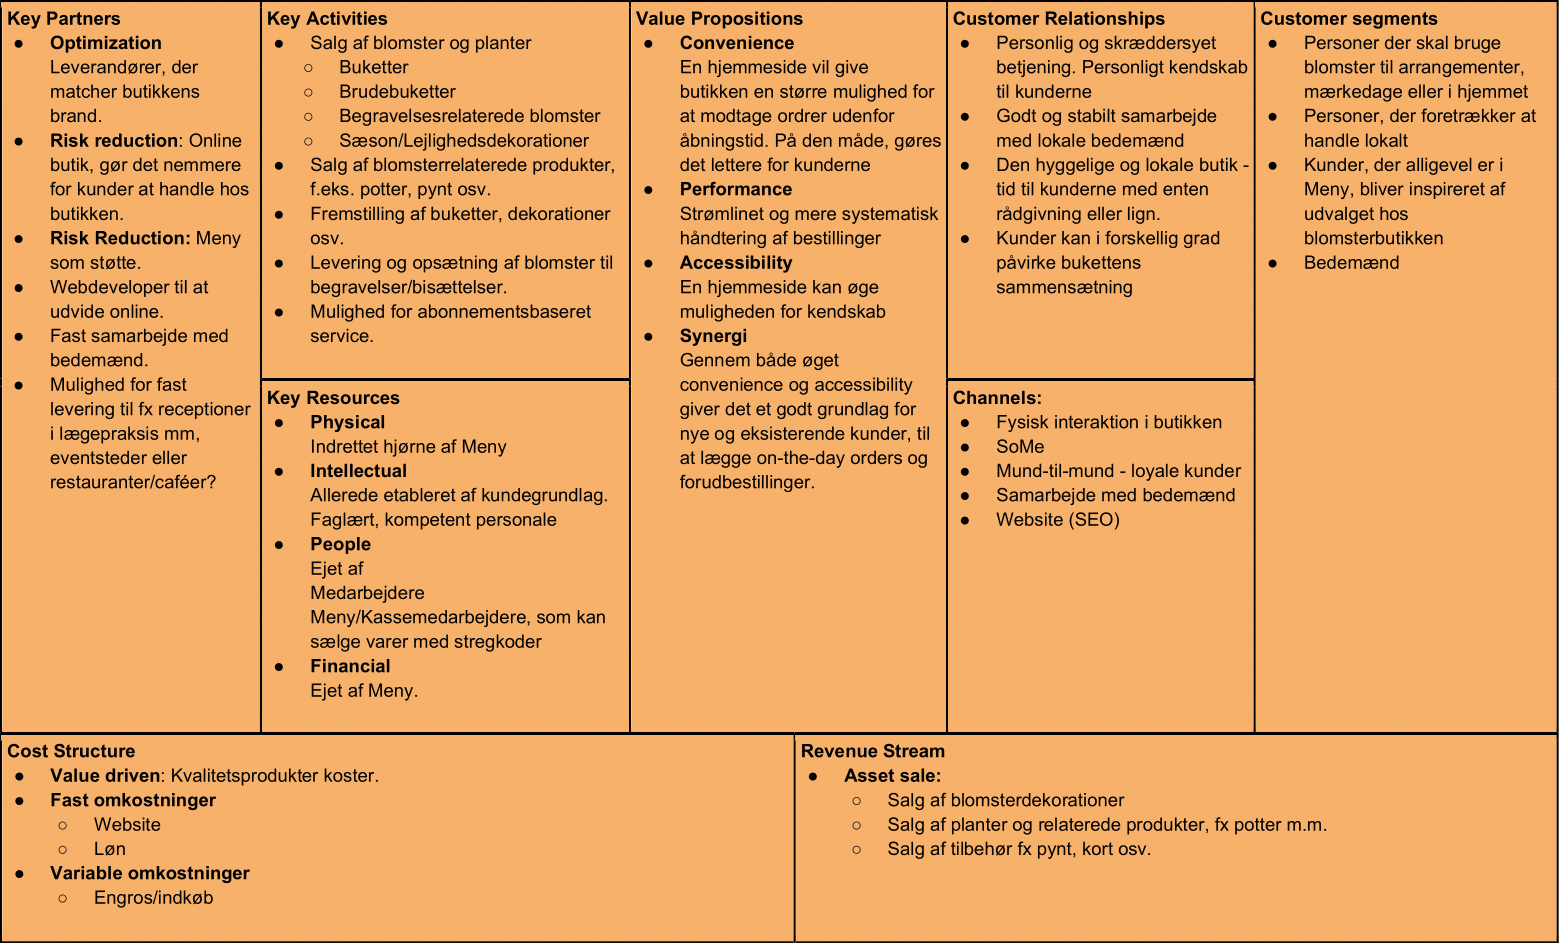
\includegraphics[width=1\textwidth]{figures/business/bmc1.png}
    \caption{Business Model Canvas for Blomsterbinderiet}
    \label{fig:bmc1}
\end{figure}

\section{Inception Deck}

\subsection{Why are we here?}
Vi vil skabe en online platform for Blomsterbinderiet, der vil transformere måden, 
hvorpå butikken kan interagere med kunder og bedemænd, ved at tilbyde en brugervenlig, 
informativ og æstetisk tiltalende webshop, styrket af personlig og effektiv service.

\subsection{Elevator Pitch}
Til blomsterbutikken, der ønsker at levere den bedste oplevelse indenfor blomsterdekorationer, 
har vi udviklet en online platform, der gør det nemt for både private og erhverv at få blomster, buketter etc, der er skræddersyet til deres behov.
Dette vil understøtte butikkens eksisterende forretning, muliggøre en udvidelse af kundegruppen samt give yderligere mulighed for at yde god service.
Selvom vores platform er online, vil den i modsætning til konkurrenterne være forankret i det lokale og den personlige service.

\subsection{Product Box}
Sammen med mockups og wireframes, er der udarbejdet en Product Box, der kan bruges til at give et overblik over produktet \ref{fig:product-box}.
\begin{figure}[H]
    \centering
    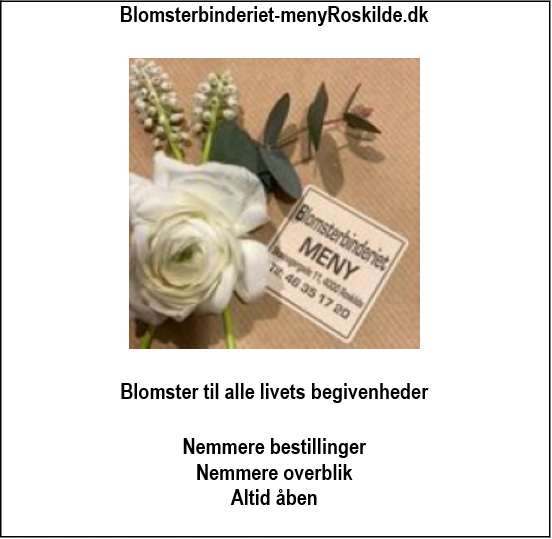
\includegraphics[width=0.4\textwidth]{figures/business/product-box.png}
    \caption{Product Box for Blomsterbinderiet}
    \label{fig:product-box}
\end{figure}

\subsection{NOT List}
For at skabe klarhed over, hvad der er i scope og hvad der er out of scope, er der udarbejdet en NOT List \ref{tab:not-list}.
\begin{table}[H]
    \centering
    \begin{tabular}{|
    >{\columncolor[HTML]{DAE8FC}}l 
    >{\columncolor[HTML]{DAE8FC}}l |}
    \hline
    \multicolumn{1}{|c|}{\cellcolor[HTML]{DAE8FC}\textbf{In Scope}}                                                                                                                                                                                                                                                                                           & \multicolumn{1}{c|}{\cellcolor[HTML]{DAE8FC}\textbf{Out of Scope}}                                                                       \\ \hline
    \multicolumn{1}{|l|}{\cellcolor[HTML]{DAE8FC}\begin{tabular}[c]{@{}l@{}}Website med modeller for produkter m.m.\\ Filtrering og sortering af udvalgte modeller\\ CRUD på udvalgte modeller\\ Database til at gemme modellerne\\ Kurv funktion\\ Ordre funktion\\ Authentication funktionalitet\\ Analyse af data fra website\end{tabular}} & \begin{tabular}[c]{@{}l@{}}Advanced security features\\ Webhosting\\ Email notifications\\ Website statestik, fx Google API\end{tabular} \\ \hline
    \multicolumn{2}{|c|}{\cellcolor[HTML]{DAE8FC}\textbf{Unresolved}}                                                                                                                                                                                                                                                                                                                                                                                                                                    \\ \hline
    \multicolumn{2}{|l|}{\cellcolor[HTML]{DAE8FC}\begin{tabular}[c]{@{}l@{}}Søgning i produkter gennem Keywords\\ Content Management System\end{tabular}}                                                                                                                                                                                                                                                                                                                                                \\ \hline
    \end{tabular}
    \caption{NOT List}
    \label{tab:not-list}
\end{table}


\subsection{Meet your neighbors}
Butiksejeren/bestyreren, der er projektets kunde (stakeholder), giver input til forretningsgang, designønsker m.m.
Personalet er de ansatte i butikken, der skal bruge platformen til at modtage og ekspedere ordre, samt kunne levere service.
Kunderne er primært private, der ønsker at købe blomster til forskellige begivenheder, fx. fødselsdage, bryllupper, begravelse etc.
Bedemændene er erhvervskunder, der ønsker at købe blomster og services ifm. begravelser.
Meny er butikkens ejer og samarbejdspartner.
Leverandørerne, der leverer blomster til butikken, er hovedsageligt et mellemled til det globale marked.
Technical/Internal Product Owner rollen vil i det her projekt blive varetaget af mig, da jeg er den eneste udvikler. Det vil afsøges om en lektor kan indgå som Product Owner til nogle sessioner.

\subsection{Show the solution}
Den foreslåede teknologiske stack og overordnede arkitektur, der skal implementeres \ref{fig:show-the-solution}. 
\begin{figure}[H]
    \centering
    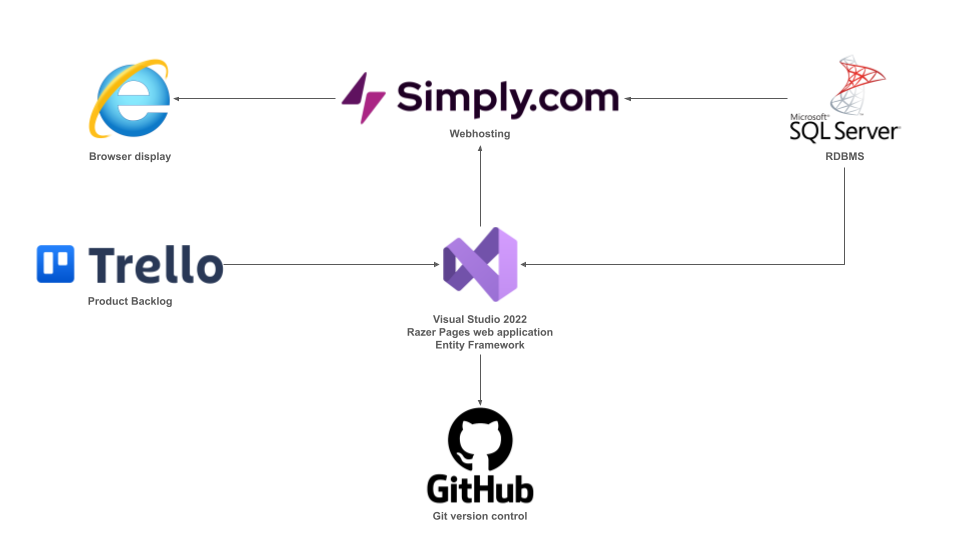
\includegraphics[width=0.75\textwidth]{figures/business/show-the-solution.png}
    \caption{The solution - billeder fra \cite{1000logos}}
    \label{fig:show-the-solution}
\end{figure}

\subsection{What keeps us up at night}
Der er identificeret nogle risikofaktorer, angivet i sandsynlighed (S) og alvorlighed (A) på en skala fra 1 til 5, hvor 1 er det laveste \ref{tab:risiko-analyse}.
\begin{table}[H]
    \centering
    \begin{tabular}{|
    >{\columncolor[HTML]{FFCCC9}}m{4.2cm} |
    >{\columncolor[HTML]{FFCCC9}}m{0.6cm} |
    >{\columncolor[HTML]{FFCCC9}}m{0.6cm} |
    >{\columncolor[HTML]{FFCCC9}}m{8.5cm} |}
    \hline
    \textbf{Risiko}             & \textbf{S} & \textbf{A} & \textbf{Mitigations Strategi}                                                                                      \\ \hline
    Begrænset tid til projektet & 5          & 5          & Der stiles mod et MVP tidligt i processen. Tasks prioriteres gennem SCRUM og der scope skaleres \\ \hline
    Tekniske udfordringer       & 4          & 3          & Projektets scope afgrænses, try-and-throw mindset og der søges ekspertviden     \\ \hline
    Begrænset personel          & 5          & 3          & Der er kun én udvikler på projektet. En disciplineret indsats er nødvendig                     \\ \hline
    For lav velocity            & 3          & 3          & Såfremt burndown chart angiver en for lav velocity, vil efterfølgende sprints rekonstrueres                  \\ \hline
    \end{tabular}
    \caption{Risiko analyse}
    \label{tab:risiko-analyse}
\end{table}

\subsection{Size it up}
Deadline er 30. maj 2024, som giver denne overordnede tidsplan \ref{list:size-it-up}.
\begin{itemize}[noitemsep]
    \item Sprint 0: 1 uge, sammenfatte og redigere eksisterende materiale
    \item Sprint 1-5: 5 uger i alt til udvikling. Der er afsat 37 timer pr. sprint
    \item Afsluttende uge: 1 uge til at sammenfatte rapporten etc
    \label{list:size-it-up}
\end{itemize}

\subsection{What is going to give}
I stedet for de klassiske sliders, er der udarbejdet en rangeret liste over features og fokusområder \ref{list:what-is-going-to-give}. 
Som på en stack er de øverste også de første, der vil blive poppet af, hvis der opstår problemer.
\begin{enumerate}[noitemsep]
    \item Website statestik, fx Google API
    \item Advanced security features
    \item Website performance optimization
    \item Email notifications
    \item Content Management System
    \item Webhosting
    \item Test (Unit test etc.)
    \item Design and layout
    \item Restrictions and requirements
    \item Søgning i produkter gennem Keywords
    \item Analyse af data fra website
    \item Kurv funktion
    \item Ordre funktion
    \item Filtrering og sortering af udvalgte modeller
    \item CRUD på udvalgte modeller
    \item Authentication funktionalitet
    \item Database til at gemme modellerne
    \item Website med modeller for produkter, ordre, kunder m.m.
    \label{list:what-is-going-to-give}
\end{enumerate}

\subsection{What it's going to take}
Grundet projektets natur er budgettet irrelevant og der vil ikke blive tilført flere udviklere.
Den eneste håndta der kan skrues på er antal timer brugt på projektet, frem mod deadline.
\chapter{SCRUM Proces}
\label{chapter:scrum}
Dette kapitel vil beskrive \emph{SCRUM}-processen, hvilke modifikationer der blev foretaget samt analysen bag og hvordan det blev anvendt til at strukturere projektet. 
I \Cref{chapter:conclusion} forefindes afsnittet \Cref{sec:conclusion_summary}, der opsummerer \emph{SCRUM}-processen og dens anvendelse i projektet.
Alle \emph{User Stories} er at finde i bilag \Cref{appendix:userstories}.

\section{Workflows}
Workflows er normalt ikke en del af \emph{SCRUM}-processen men en metode, hvorpå jeg kunne tage noget, der var i størrelsen af en \emph{epic user story} og dele den op i mindre \emph{User Stories}. 
Jeg har valgt at bruge denne metode, da den låner elementer fra \emph{Persona}-tilgangen, men i et format, der gør det mere håndgribeligt at omsætte til \emph{User Stories}.
Samtidig giver det et fokus på funktionalitet for slutbrugeren og det design, der skal støtte op om det.

\subsection{Workflow eksempel}
Situation: Medarbejder (blomsterdekoratør) ekspederer en ordre.
Formål: At håndtere indkommende ordrer og forberede blomsterarrangementer.
\begin{enumerate}
    \item Medarbejder logger ind på ordreportalen.
    \item Medarbejder gennemser listen over dagens ordrer og vælger en ordre til ekspedition.
    \item Medarbejder forbereder blomsterarrangementet i henhold til kundens specifikationer.
    \item Medarbejder markerer ordren som 'klar til levering' eller 'klar til afhentning'.
    \item Medarbejder opdaterer ordrestatus i systemet.
    \label{item:workflow-eksempel}
\end{enumerate}

\begin{figure}[H]
    \centering
    \begin{minipage}[b]{0.45\textwidth}
        \centering
        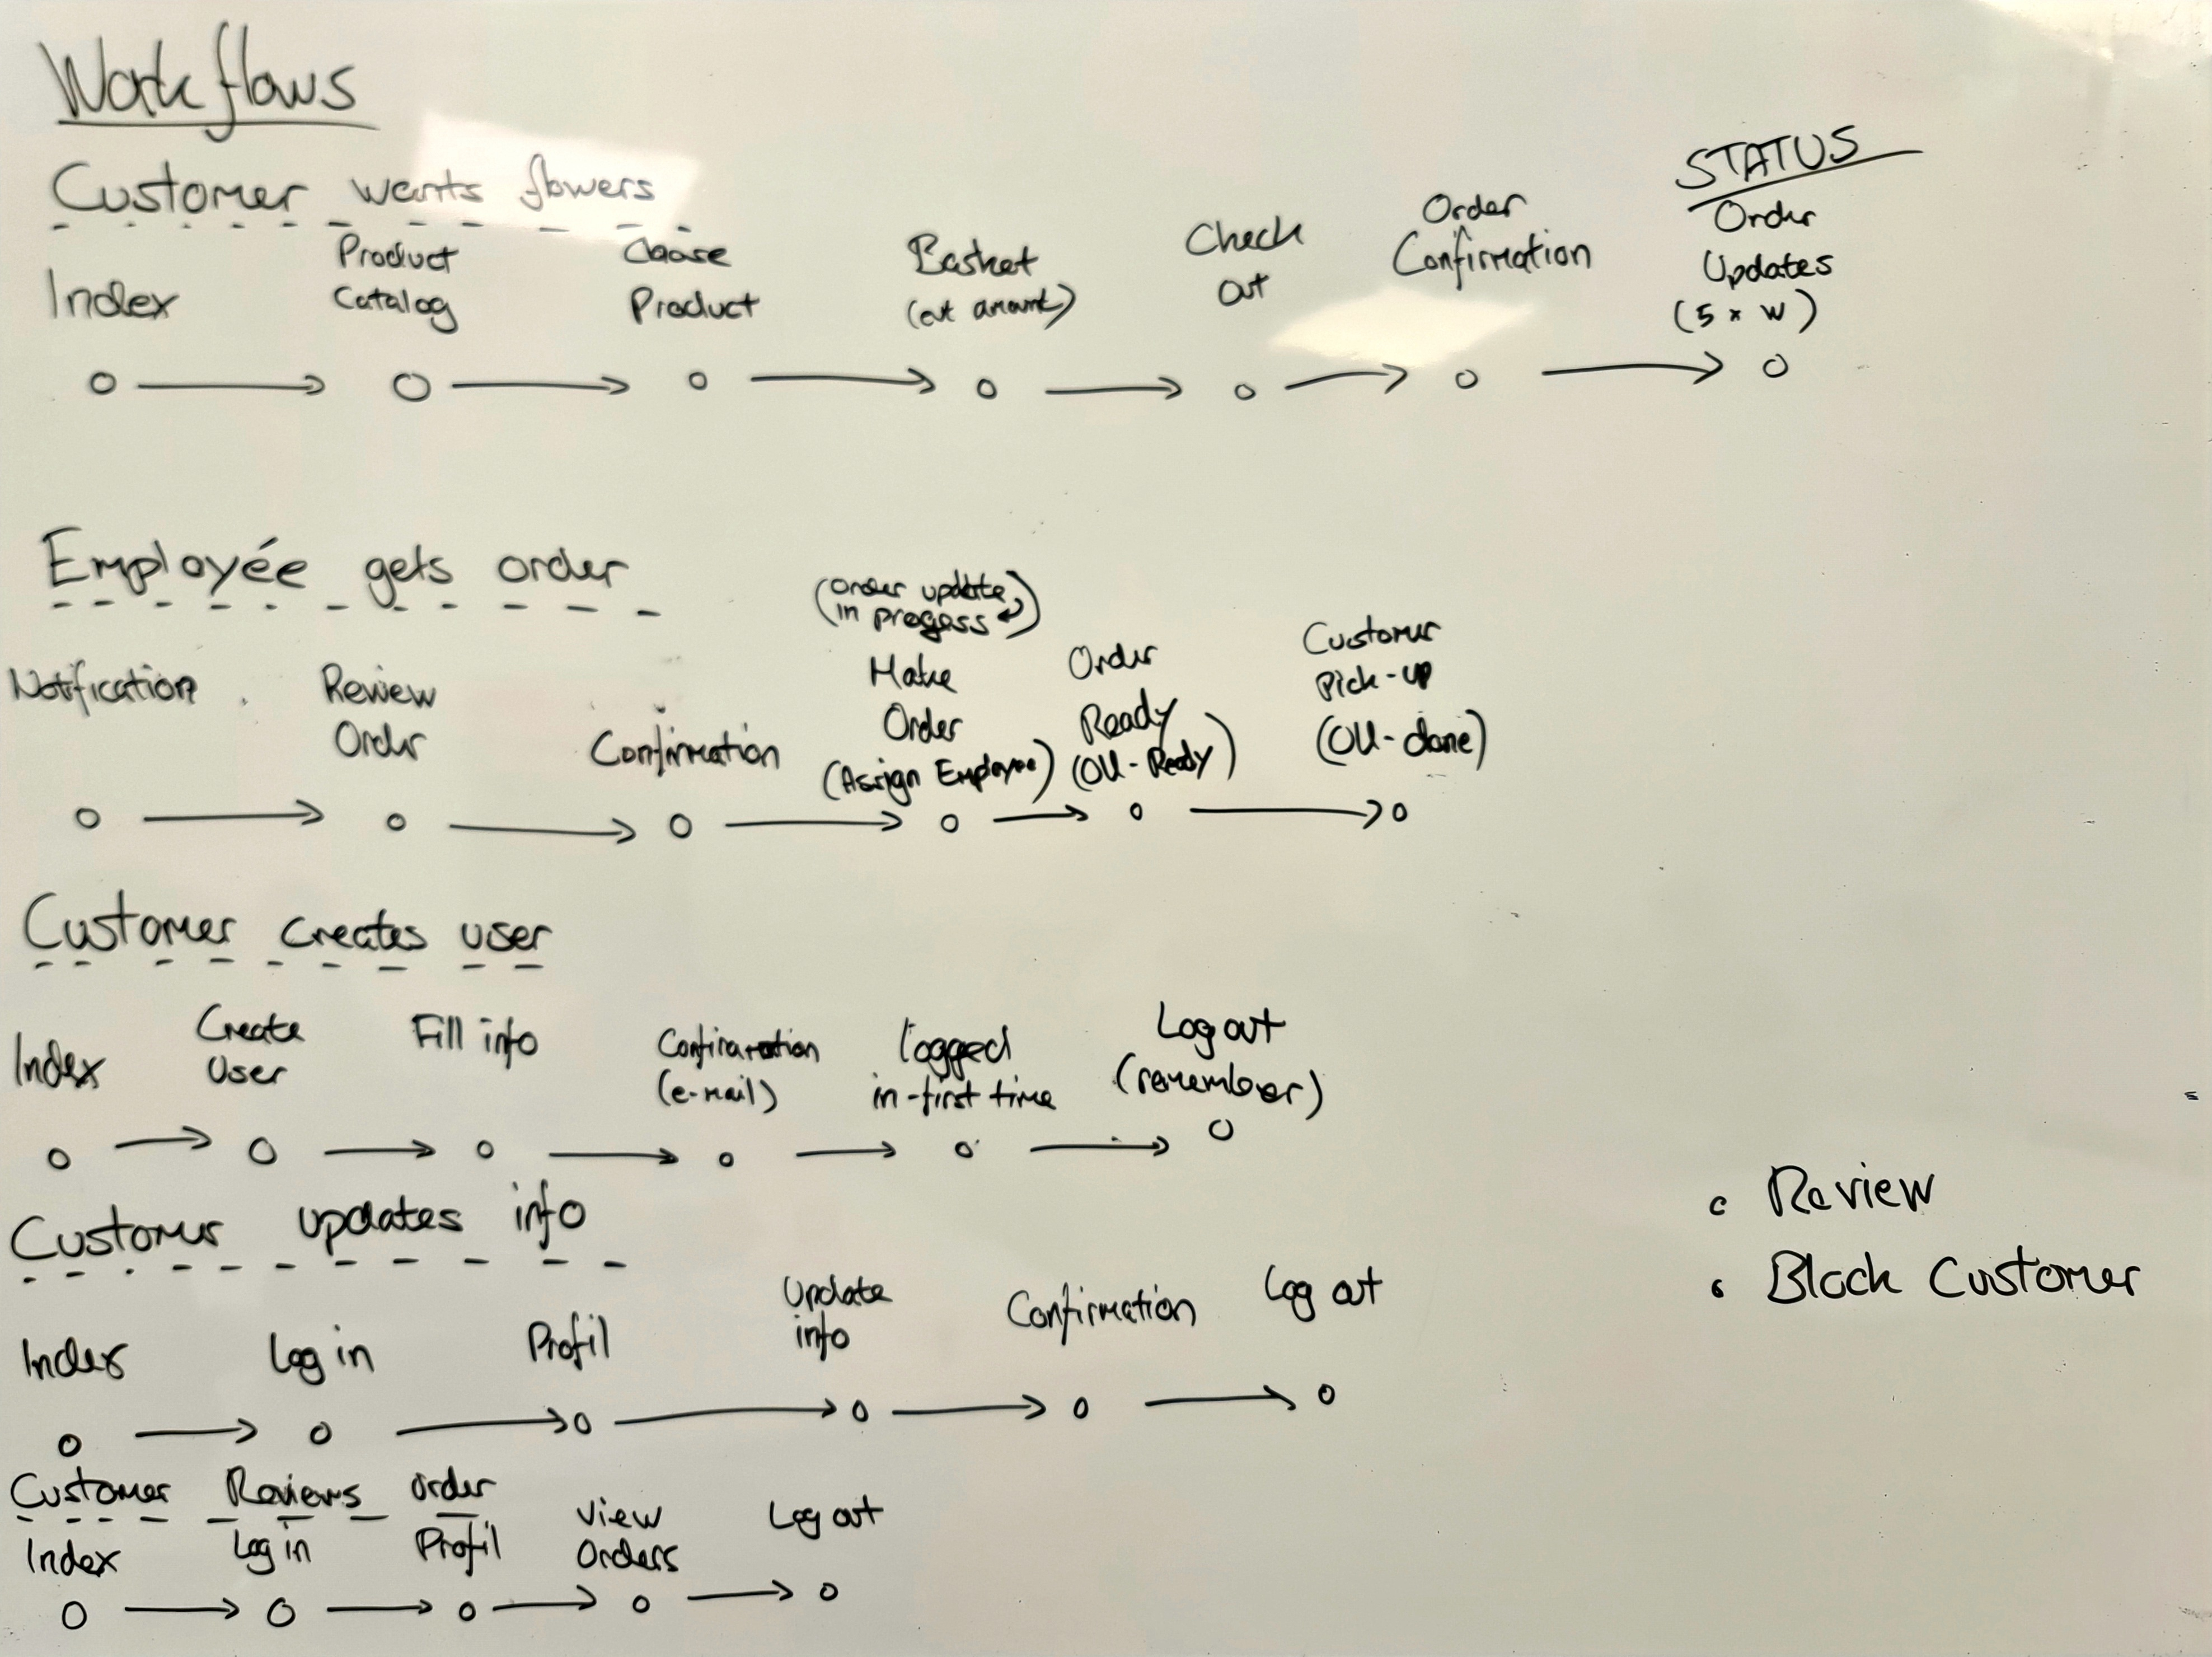
\includegraphics[width=\textwidth]{figures/scrum/workflow-board1.jpg}
        \caption{Workflow Board 1}
        \label{fig:workflow-board1}
    \end{minipage}
    \hfill
    \begin{minipage}[b]{0.45\textwidth}
        \centering
        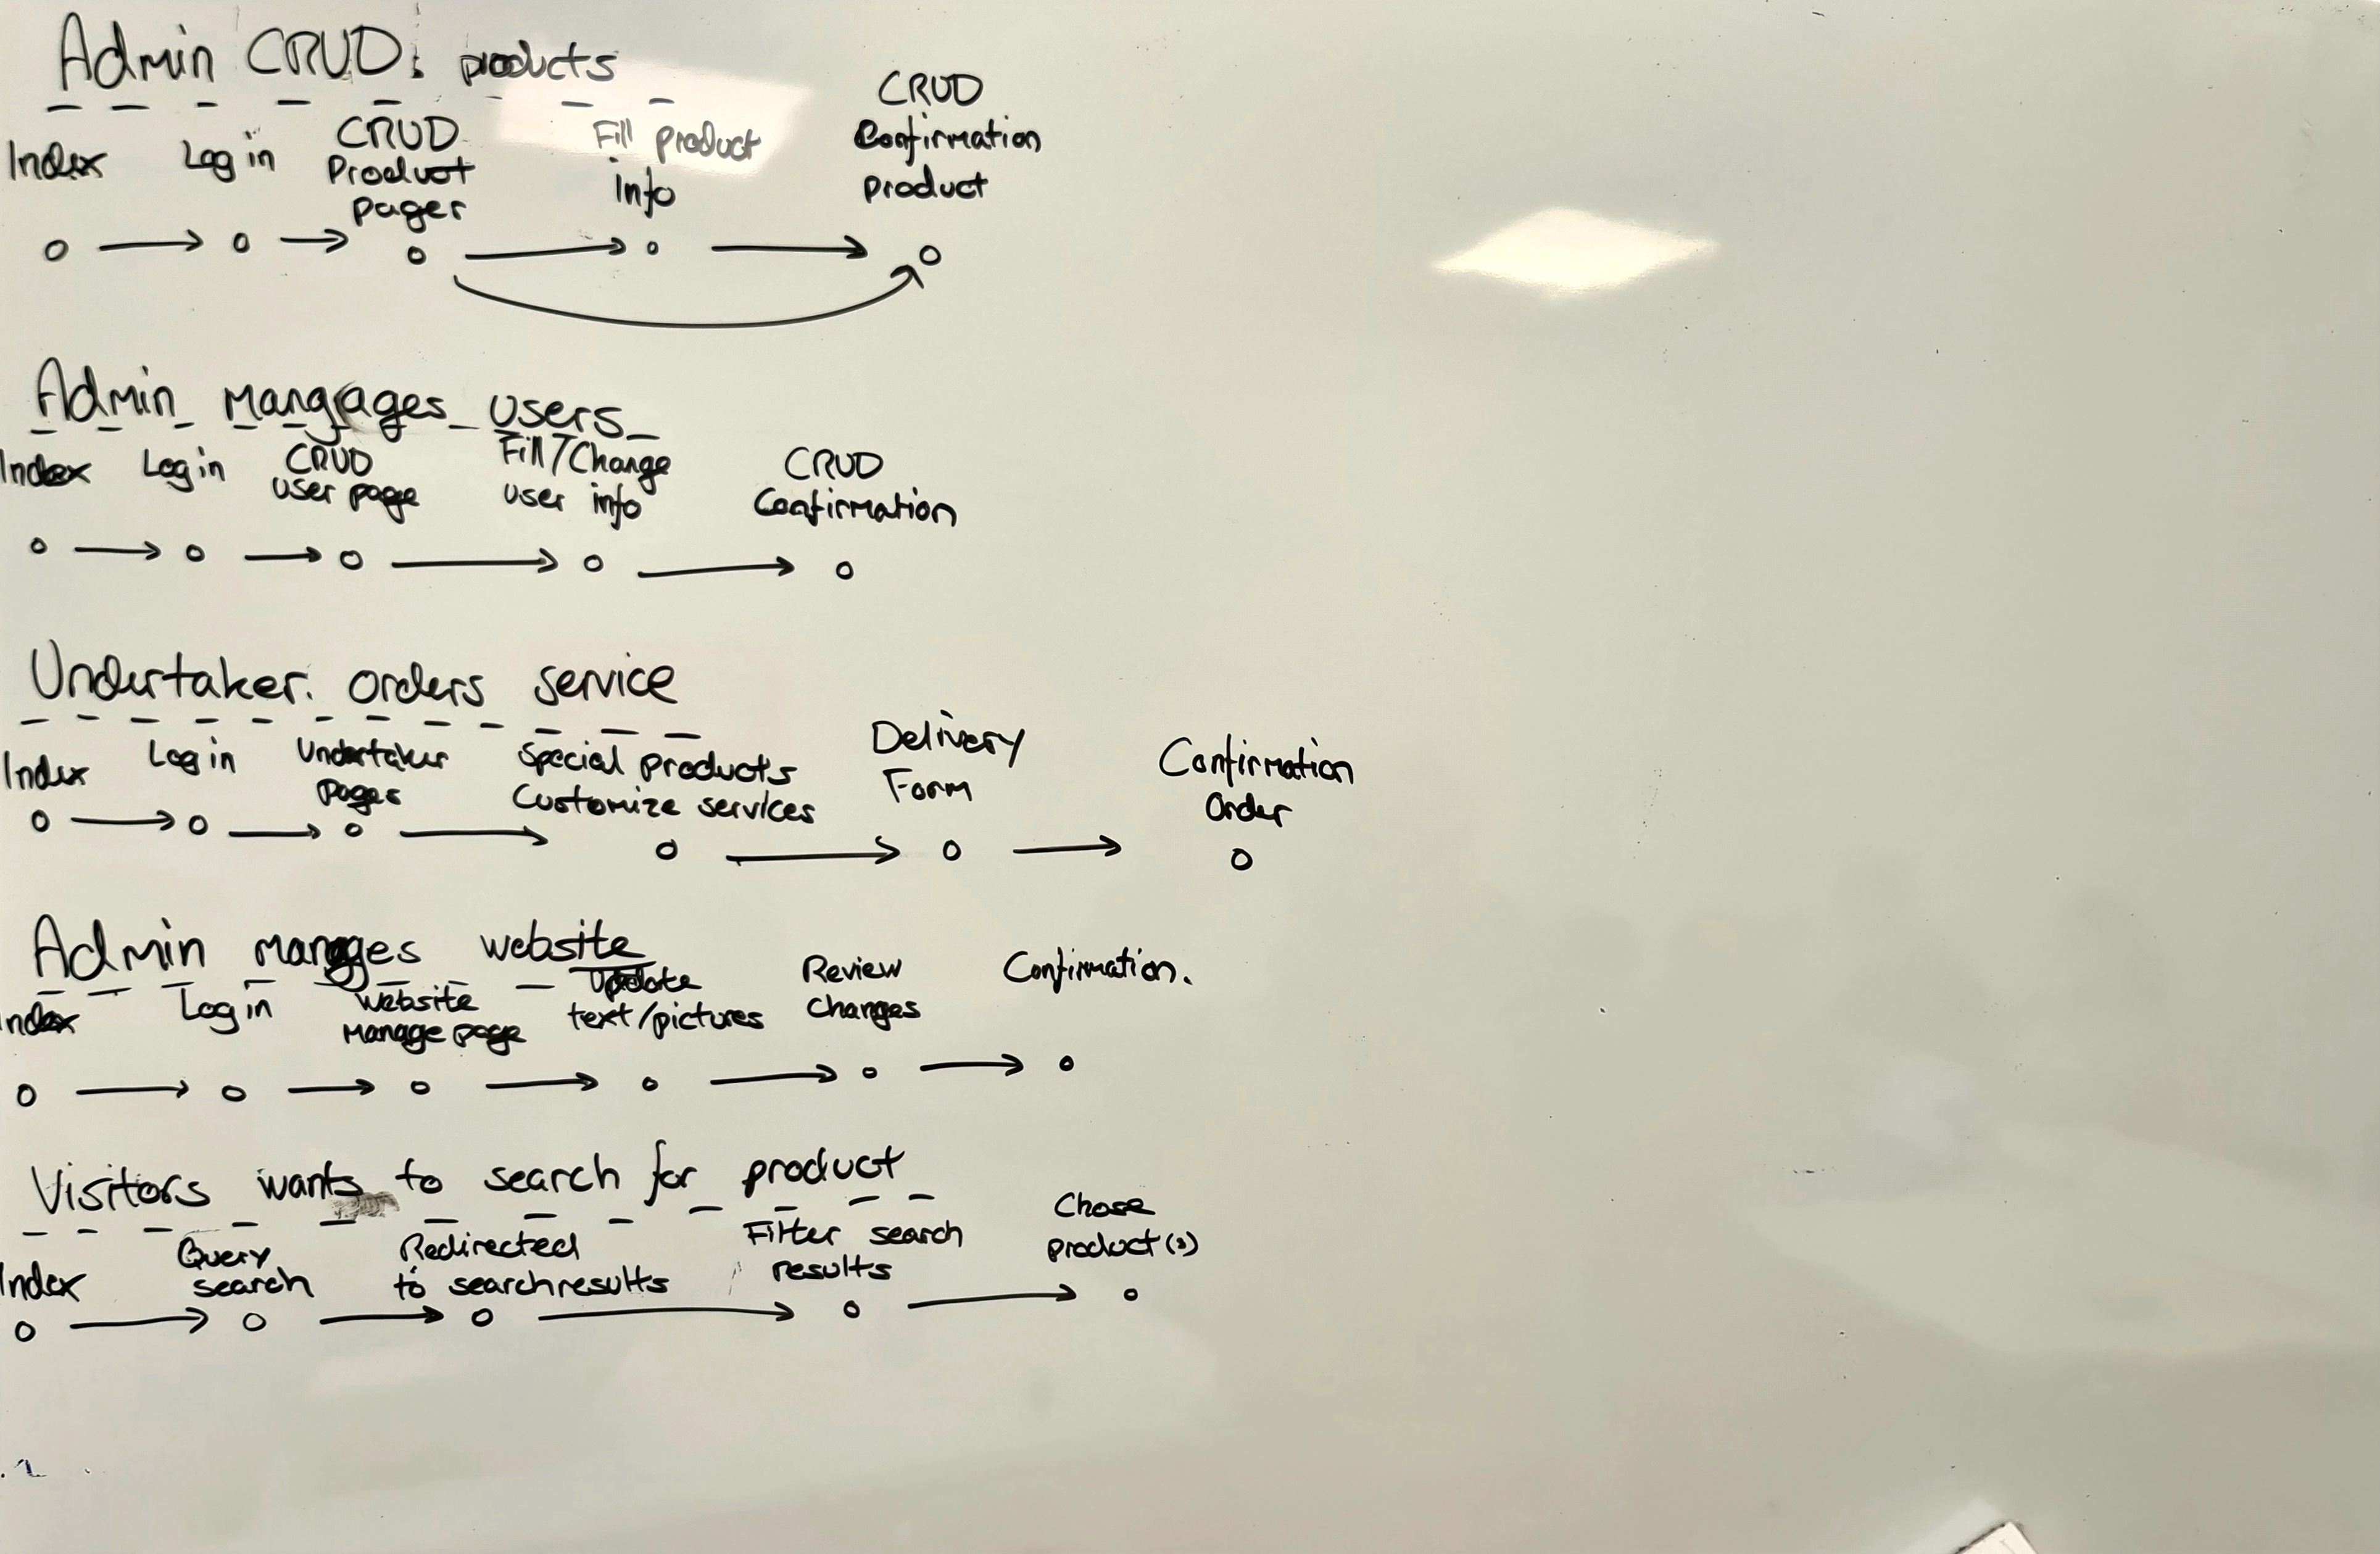
\includegraphics[width=\textwidth]{figures/scrum/workflow-board2.jpg}
        \caption{Workflow Board 2}
        \label{fig:workflow-board2}
    \end{minipage}
\end{figure}

Rent fysisk blev de opskrevne Workflows sat op på en whiteboard. Herefter blev der sat ringe om områder, der kunne omsættes til \emph{User Stories}.
Workflow-punkter, der gik igen eller ville afføde den samme funktionalitet, blev overstreget og samlet i en \emph{User Story}.
I eksemplet fra \Cref{item:workflow-eksempel} kunne det være følgende \emph{User Stories}:
\begin{enumerate}
    \item "Som medarbejder vil jeg kunne logge ind på ordreportalen, så jeg kan ekspedere ordrer."
    \item "Som medarbejder vil jeg kunne se ordredetaljer om blomsterarrangementet, så jeg kan ekspedere ordrer."
    \item "Som medarbejder vil jeg kunne opdatere ordrestatus, så jeg kan tydeliggøre for alle brugere, hvor langt ordren er."
    \label{item:workflow-us-eksempel}
\end{enumerate}

\begin{figure}[H]
    \centering
    \begin{minipage}[b]{0.45\textwidth}
        \centering
        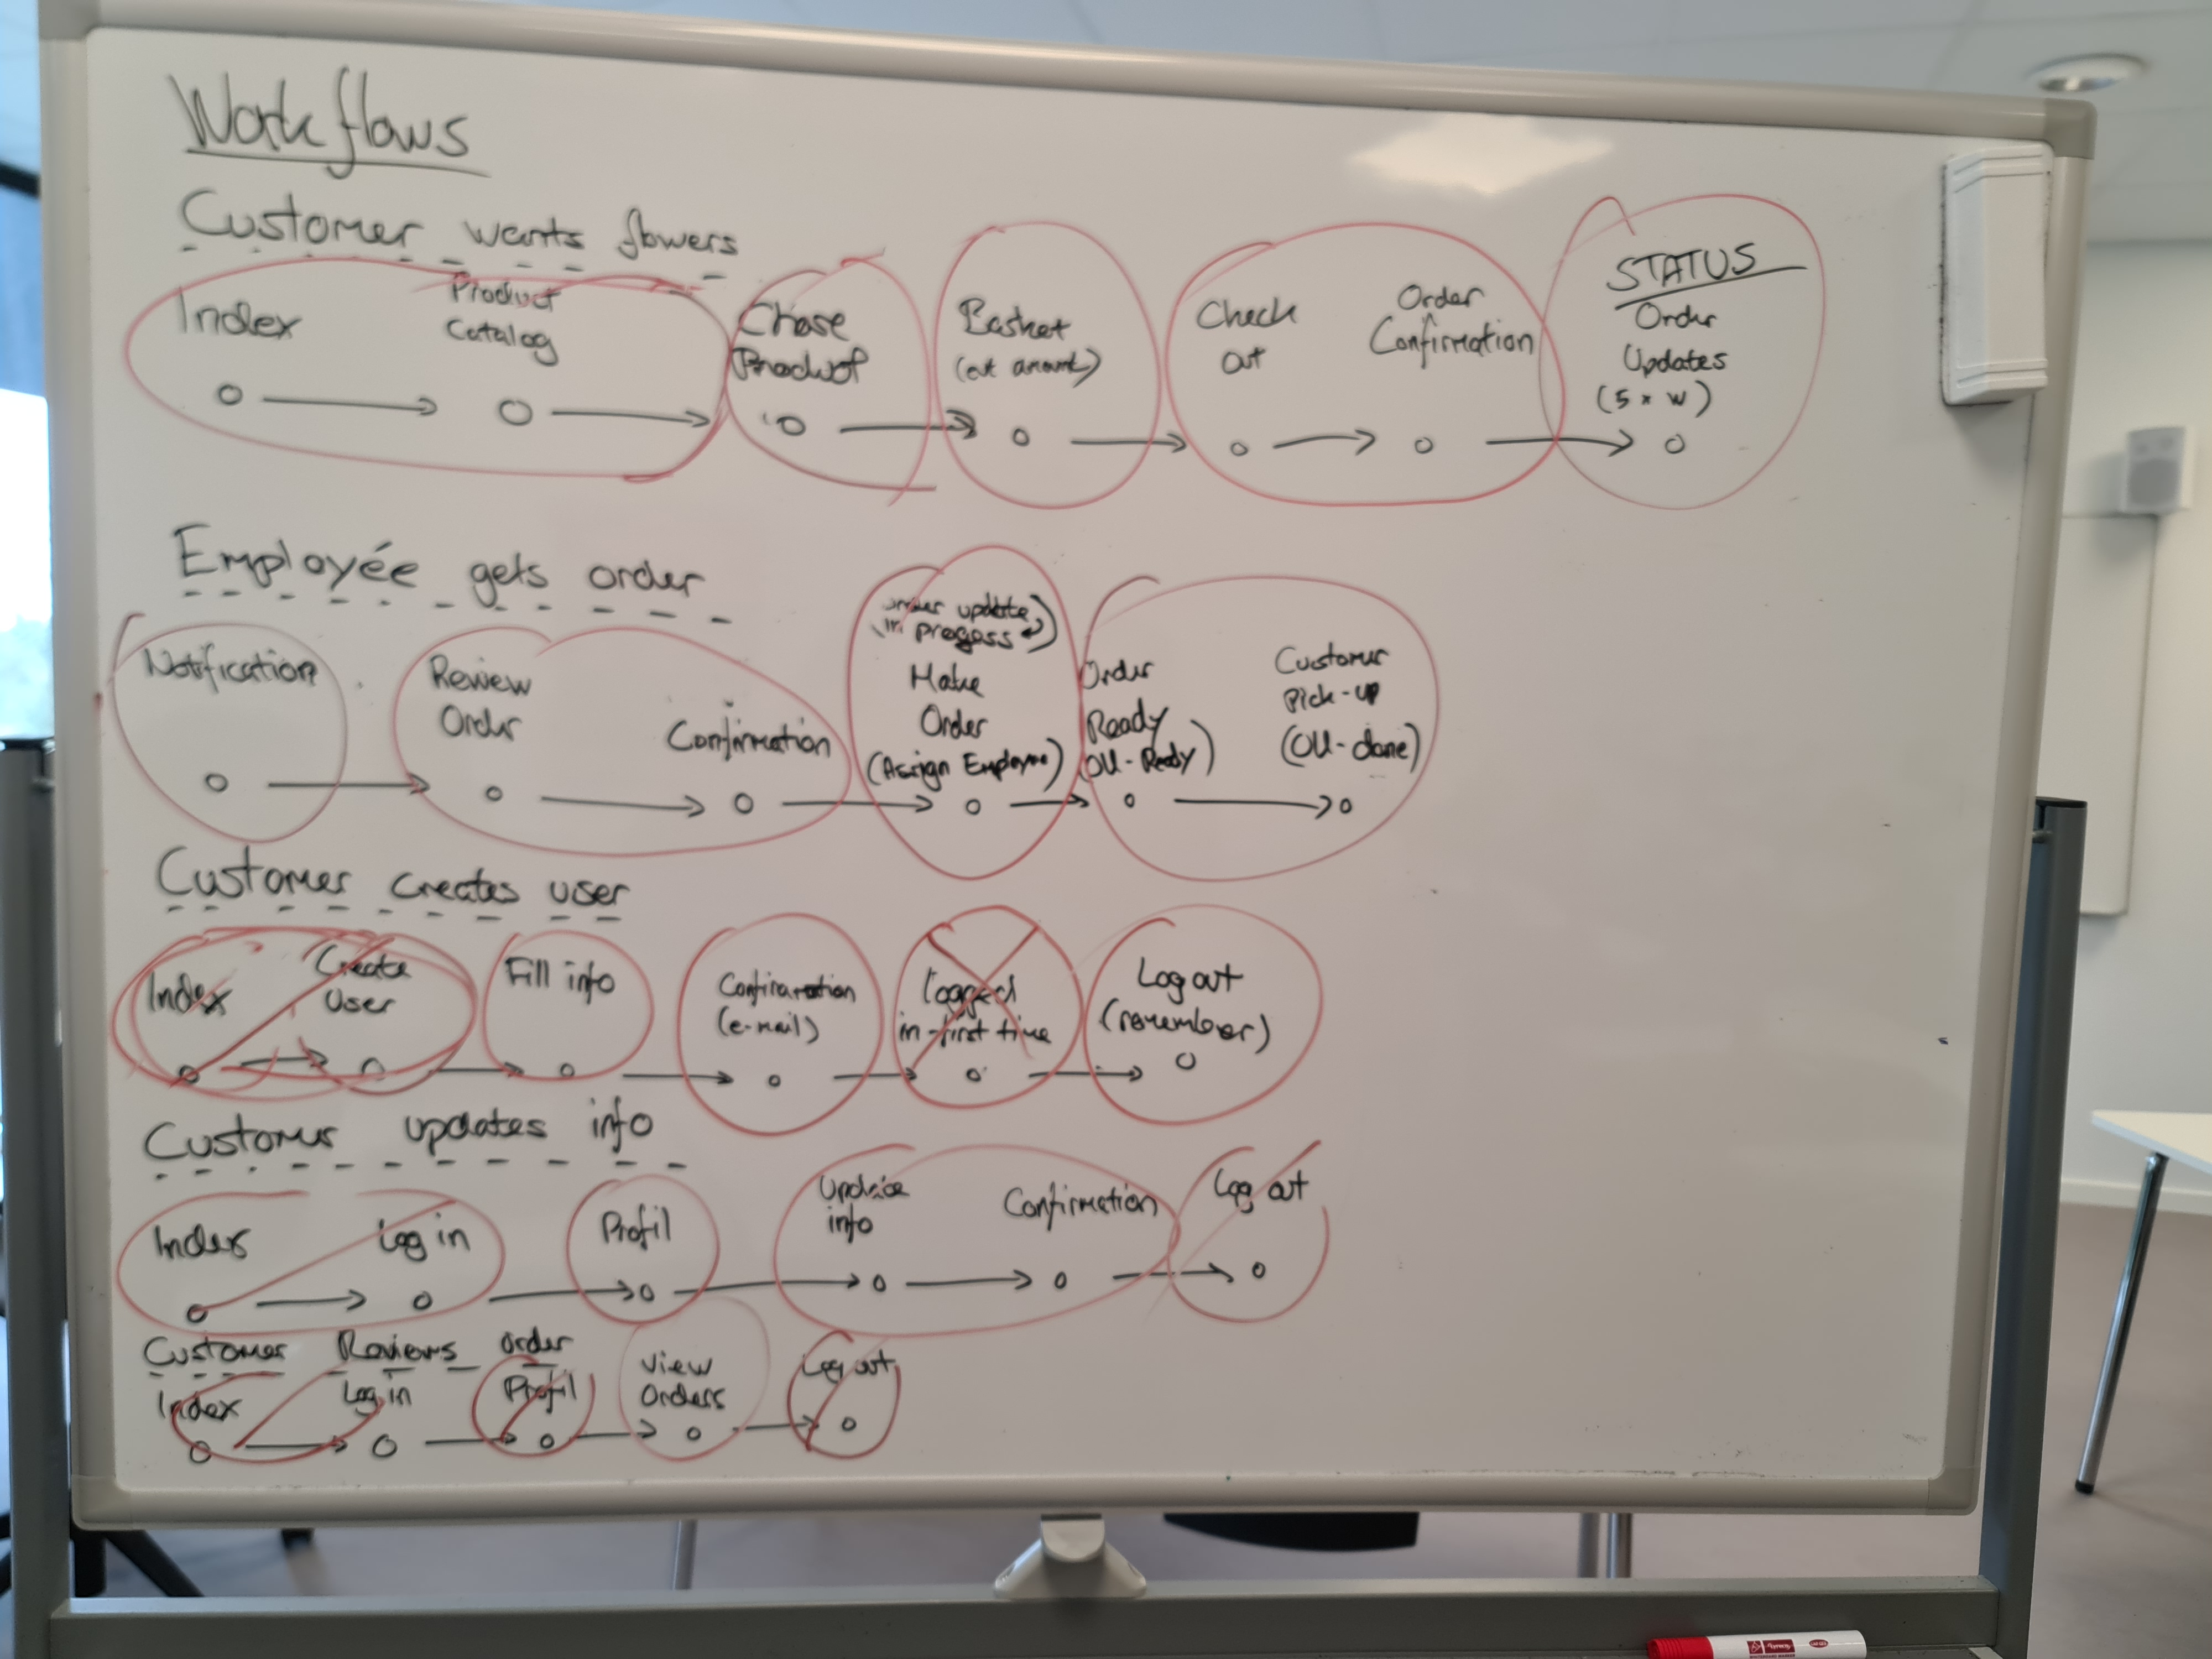
\includegraphics[width=\textwidth]{figures/scrum/workflow-board-red-rings1.jpg}
        \caption{Workflow Board 1}
        \label{fig:workflow-board-red-ring1}
    \end{minipage}
    \hfill
    \begin{minipage}[b]{0.45\textwidth}
        \centering
        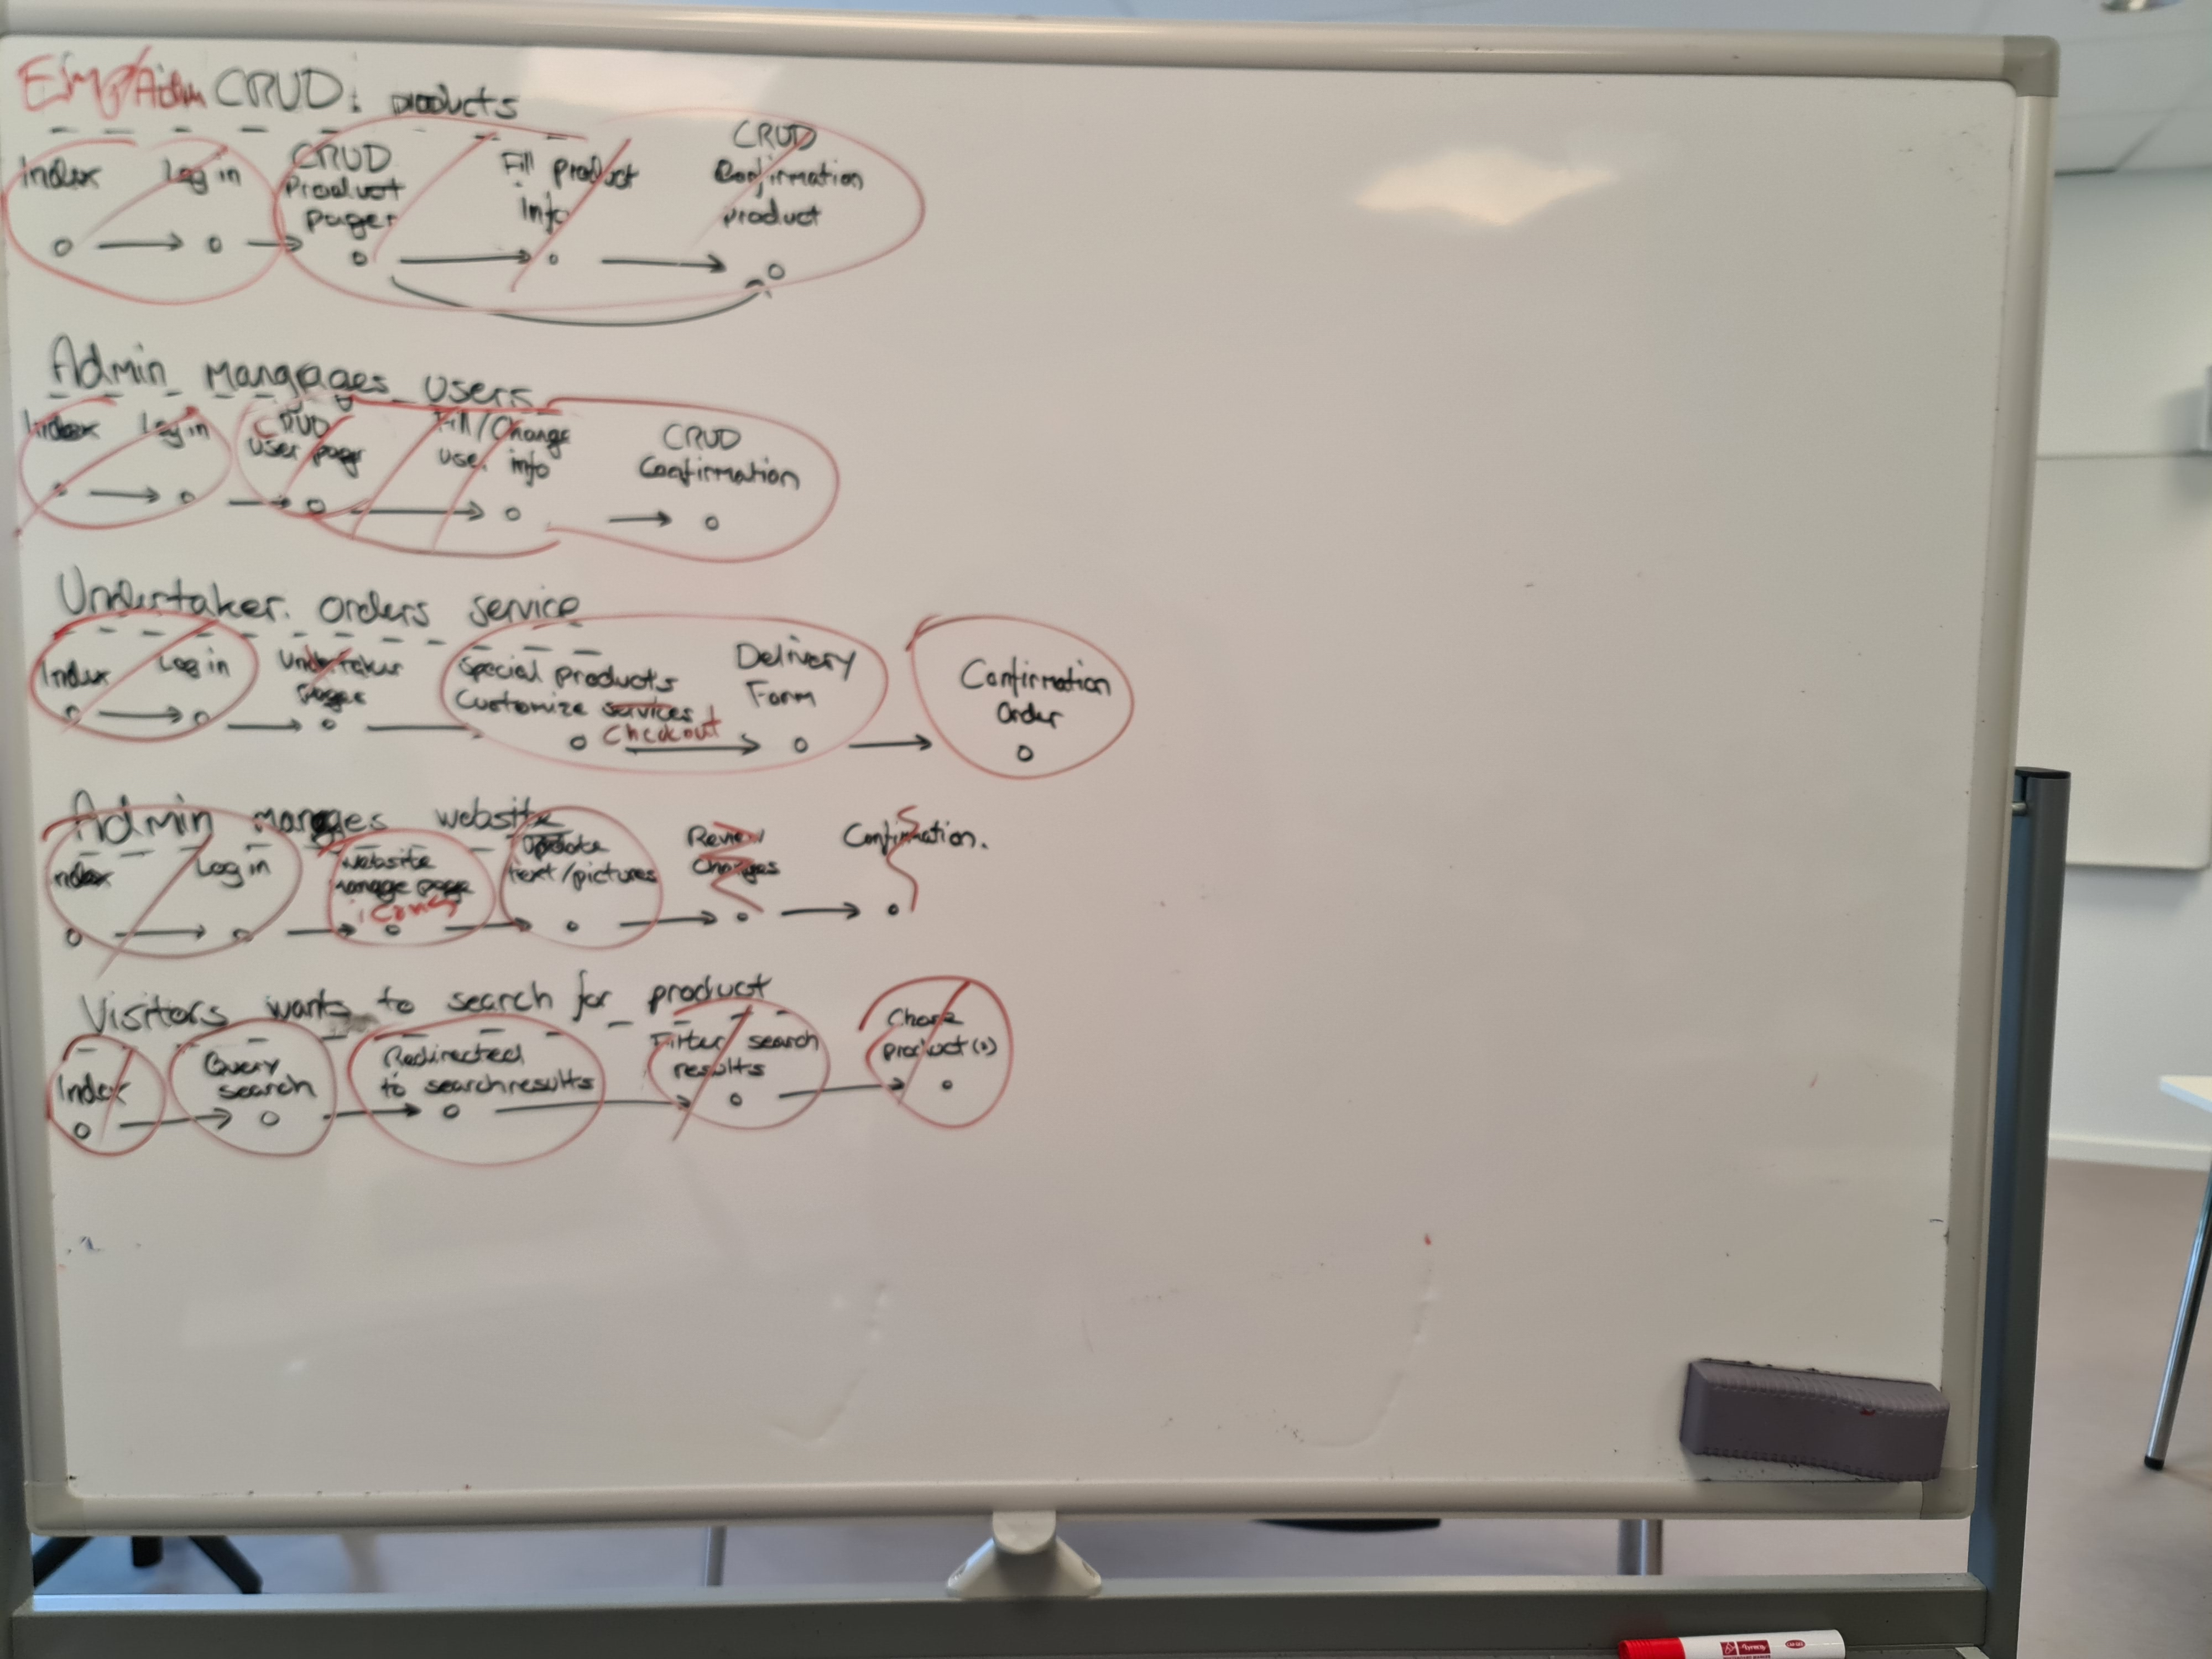
\includegraphics[width=\textwidth]{figures/scrum/workflow-board-red-rings2.jpg}
        \caption{Workflow Board 2}
        \label{fig:workflow-board-red-ring2}
    \end{minipage}
\end{figure}

Dette er stadig relativt store \emph{User Stories}. Ved at tilknytte \emph{Tasks} til hver \emph{User Story}, bliver de mere overskuelige og 
nemmere at tildele \emph{Acceptance Criteria}. Dermed får man et godt overblik over, hvad der skal til for at implementere funktionaliteten.

\section{User Stories}
Der blev skrevet \emph{User Stories} for kunder (underforstået private), bedemænd, medarbejdere og bestyrer, da de har forskellige behov og derfor også forskellige \emph{User Stories}.
Da hensigten med \emph{User Stories} er at beskrive funktionalitet fra slutbrugerens perspektiv, vil nogle elementer overlappe. Det kan f.eks. være, at både en medarbejder og en kunde kunne logge ind på webshoppen.
I sådanne tilfælde blev der skrevet en \emph{User Story} for hver, hvis de havde forskellige behov og derfor også forskellige \emph{Acceptance Criteria}.
Ved for stort overlap blev de slået sammen til en \emph{User Story}, der dækkede begge brugere.

\subsection{Opbygning af User Stories}
\emph{User Stories} blev skrevet i formatet "Som [rolle] ønsker jeg [handling], med det formål [resultat]".
Dette format sikrer, at \emph{User Stories} er fokuseret på funktionalitet og ikke teknologi.
Derudover blev der tilføjet \emph{Tasks} for at give klarhed til udvikleren om, hvad der konkret skulle gøres, samt \emph{Acceptance Criteria} for at sikre, at \emph{User Stories} var klare og præcise.

\subsection{Prioritering af User Stories}
\emph{User Stories} blev indledende prioriteret efter \emph{MoSCoW}-metoden, hvor de blev inddelt i fire kategorier: Must have, Should have, Could have og Won't have.
Det var dog ikke givende, da scope allerede var blevet afgrænset. Derfor blev \emph{User Stories} prioriteret efter, hvad der var vigtigst for slutbrugeren og med henblik på, at der hurtigt skulle kunne leveres en funktionel kerne af produktet.
\emph{User Stories} uden for scope forblev som "gode ideer" i \emph{product backloggen}.

\subsection{Estimering af User Stories}
\emph{User Stories} blev indledende estimeret i \emph{T-shirt sizes} efter XS, S, M, L, XL. Dette blev gjort for at fjerne fokus fra en numerisk værdi og i stedet fokusere på, hvor kompleks en \emph{User Story} var.
Estimeringen endte med at anvende \emph{Story Points} efter Fibonacci-sekvensen 1, 2, 3, 5 og 8. Dette skift skete, da det var nemmere at anvende tal, når bl.a. \emph{velocity} skulle beregnes.
Estimeringen tog udgangspunkt i tre faktorer:
\begin{itemize}
    \item Kodemængde, da overskuelighed forsvinder i takt med, at koden vokser, så risikoen for fejl stiger, og hvor lang tid debugging vil tage øges.
    \item Kodekompleksitet, baseret bl.a. på hvorvidt der skulle anvendes (mange) komplekse datatyper, eksotiske libraries som f.eks. \emph{httpContext}, eller der var mange afhængigheder.
    \item Funktionalitetskompleksitet, forstået som et holistisk skøn på, hvor mange delelementer denne feature ville gribe ind i, men bl.a. også hvor mange \emph{guardrails}, der skulle tilføjes for at sikre, at funktionaliteten virkede som forventet.
\end{itemize}
\emph{Planning Poker} blev anvendt i det gamle team til at estimere \emph{User Stories}. Hensigten var, at det skulle sikre, at alle i teamet havde en stemme, og at der blev taget højde for alle synspunkter.
Dette virkede redundant i det nye team, da der kun var én udvikler, der skulle estimere.

\subsection{User Story Mapping}
\emph{User Story Mapping} er en metode til at prioritere \emph{User Stories} og få et overblik over, hvad der skal implementeres først.
Det er en metode, der tager udgangspunkt i slutbrugerens behov og dermed sikrer, at de vigtigste funktionaliteter bliver implementeret først.
Her hjalp Workflows også med at identificere \emph{User Stories}, der kunne grupperes og prioriteres, fordi de netop beskrev en holistisk proces.
I eksemplet fra \Cref{item:user-story-mapping-eksempel} kunne det være, at \emph{User Stories} 1, 2, 3, 4 og 9 skulle implementeres først, da de dækker overordnede funktionaliteter, der er vigtige for kunden.

\subsubsection{User Story Mapping eksempel}
Kunden ønsker at kunne logge ind og se sine ordrer og betalinger. Dette kræver, at kunden kan logge ind, se en oversigt over sine ordrer, se en oversigt over sine betalinger og se detaljer om en ordre.
\begin{enumerate}
    \item "Som kunde vil jeg kunne logge ind, så jeg kan se mine ordrer og betalinger."
    \item "Som kunde vil jeg kunne se en oversigt over mine ordrer, så jeg kan følge med i, hvor langt de er."
    \item "Som kunde vil jeg kunne se en oversigt over mine betalinger, så jeg kan se, hvad jeg har betalt."
    \item "Som kunde vil jeg kunne se detaljer om en ordre, så jeg kan se, hvad jeg har betalt for."
    \item "Som kunde vil jeg kunne se en oversigt over mine personlige oplysninger, så jeg kan se, hvad I har registreret om mig."
    \item "Som kunde vil jeg kunne se detaljer om mine personlige oplysninger, så jeg kan se, hvad I har registreret om mig."
    \item "Som kunde vil jeg kunne ændre mine personlige oplysninger, så jeg kan sikre, at de er korrekte."
    \item "Som kunde vil jeg kunne slette mine personlige oplysninger, så jeg kan sikre, at de ikke længere er tilgængelige."
    \item "Som kunde vil jeg kunne logge ud, så jeg kan sikre, at mine oplysninger ikke er tilgængelige for andre."
    \label{item:user-story-mapping-eksempel}
\end{enumerate}

\subsection{Product backlog}
Da tidsrammen for projektet var begrænset, blev der oprettet en \emph{Product Backlog}, der indeholdt alle \emph{User Stories}. Derfra blev der dog lavet en iterativ \emph{Sprint Planning} for hele projektet for at sikre, at scope for projektet var realistisk.
Alle \emph{User Stories} blev prioriteret og estimeret samt fordelt i de fem \emph{Sprints} i en prioriteret rækkefølge med de vigtigste på toppen, se figur \Cref{fig:trello-sprint-backlogs}. 
Dette skabte overblik over, hvad der skulle implementeres først, samt satte en indsats/belastning, både på \emph{Sprint} basis men også for hele projektet.
Dermed kunne det bruges som et styringsredskab til at sikre, at projektet blev færdigt til tiden.
\begin{figure}[H]
    \centering
    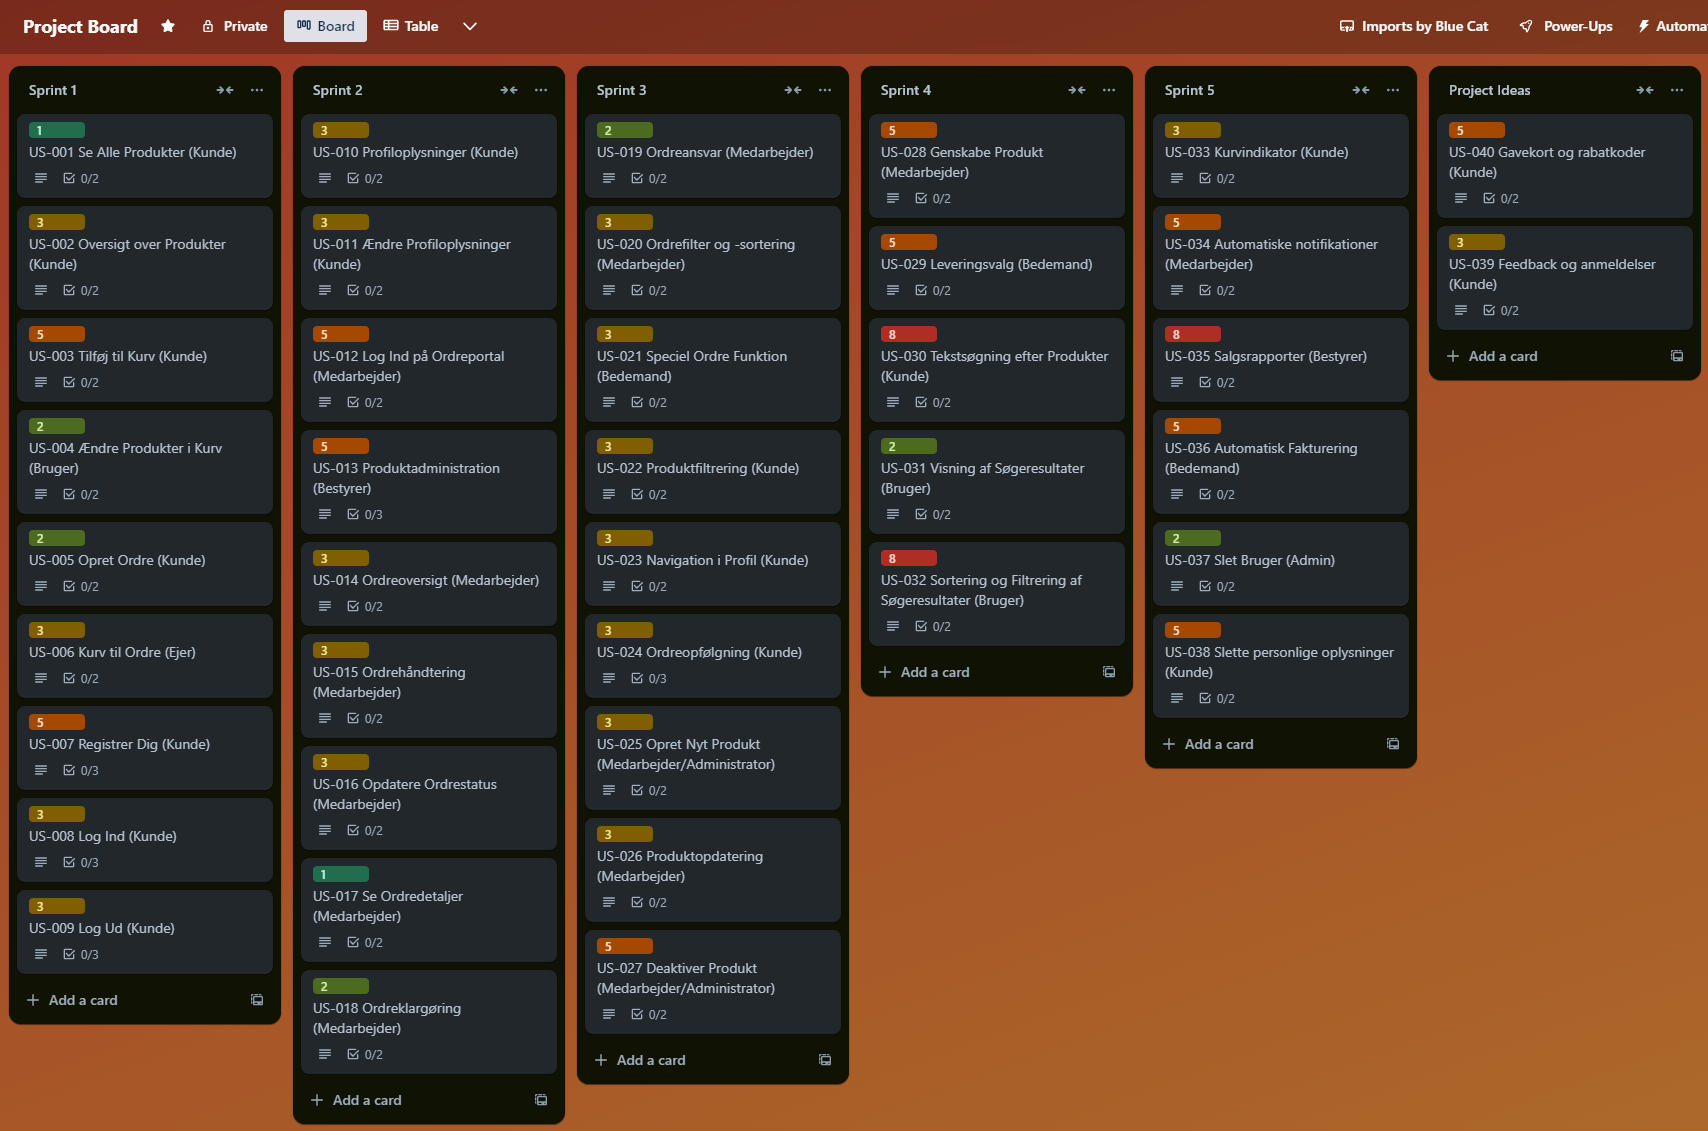
\includegraphics[width=0.9\textwidth]{figures/scrum/trello-sprint-backlogs.png}
    \caption{\emph{Product Backlog}}
    \label{fig:trello-sprint-backlogs}
\end{figure}

\section{Sprints}
\emph{Sprints} blev planlagt til at vare én uge, da det var en passende længde til at kunne implementere en vis mængde \emph{User Stories} (med tilhørende debugging, dokumentation etc.), men kort nok til at få en fornemmelse af \emph{velocity}.

\subsection{Sprint Planning}
\emph{Sprint Planning} blev en mere organisk, iterativ proces, med udgangspunkt i den første estimering og fordeling på \emph{Sprints}. 
Pointer fra \emph{Sprint Reviews} blev brugt til efterfølgende \emph{Sprint Planning}, så der blev taget højde for eventuelle forsinkelser eller overestimeringer.

\subsection{Daily Standup}
\emph{Daily Standup} blev mere til en daglig refleksion, da der kun var én udvikler. Da softwareudvikling ind imellem kræver den "gode idé" eller samtaler med ens gummiand, så blev der også taget højde for, om der skulle bruges kræfter andetsteds.
Der kunne stadig dokumenteres m.m. som ikke nødvendigvis var en del af den daglige udvikling.

\subsection{Sprint Review}
\emph{Sprint Review} blev brugt til at reflektere og evaluere, hvad der var blevet implementeret og hvad der manglede. Det blev også brugt til at justere \emph{Product Backloggen}, hvis der var \emph{User Stories}, der ikke længere var relevante eller \emph{User Stories}, der skulle tilføjes.
\emph{Burndown Chart} blev brugt til at visualisere og bestemme \emph{velocity} for \emph{Sprintet} og projektet som helhed.

\subsection{Sprint Retrospective}
\emph{Sprint Retrospective} var mere en selvransagelse end en gruppediskussion, da der kun var én udvikler. Der var dog stadig fokus på, hvad der var gået godt, og hvad der kunne forbedres. 
Bl.a. blev der reflekteret over, om der var \emph{User Stories}, der var over- eller underestimeret, og hvad der kunne gøres for at forbedre det. 
Et andet eksempel var, om der var blevet lagt en for stor indsats i en bestemt implementering og hvornår det gik fra, at ville finde en løsning til at ville "besejre" et problem.

\section{Burndown Chart}
\emph{Burndown Chart} blev brugt til at visualisere, hvor mange \emph{Story Points} der var tilbage i \emph{Sprintet} og projektet som helhed.

\section{Velocity}
\emph{Velocity} blev brugt til at estimere, hvor mange \emph{User Stories} der kunne implementeres i et \emph{Sprint}, og dermed hvor mange \emph{User Stories} der kunne implementeres i projektet som helhed.
\emph{Velocity} blev beregnet som gennemsnittet af de seneste \emph{Sprints}, da det gav et mere retvisende billede af, hvor mange \emph{Story Points} der kunne implementeres i et \emph{Sprint}.
\chapter{Software Design}
\label{chapter:software-design}

\section{Domain Model Diagram}
Det første skridt i designprocessen er at lave et Domain Model Diagram (DMD). Det er vigtigt at bemærke følgende:
\begin{itemize}
    \item DMD forholder sig til den virkelige verdens koncepter og relationer
    \item DMD er en statisk model, der ikke tager højde for ændringer i systemet over tid
    \item DMD anvender \emph{entities} til at repræsentere konceptuelle klasser
    \item DMD anvender \emph{relations} til at vise, hvordan \emph{entities} er relateret til og interagere med hinanden på et konceptuelt plan
    \item DMD kan bruges til at skabe en fælles forståelse af projektet og identificere de vigtigste klasser og \emph{relations}
    \item DMD kan bruges til at skabe en bedre forståelse af problemet for udviklerne og dermed en bedre løsning
    \item DMD kan bruges til at identificere de vigtigste klasser og deres \emph{relations}
    \item DMD er ikke en teknisk model og kan ikke direkte implementeres i software
\end{itemize} 
Kontrast skal primært ses i forhold til et Domain Class Diagram, hvor hver klasse har attributter, metoder og er forbundet andre klasser gennem specificerede relationer (fx agrregation) og mulitplicitet. 
Ligeledes ville man i et DCD se klasserne Basket, BasketItem og BasketSerice, muligvis med et IBasketService interface som implementeringen af konceptet "Kurv".
Det er vigtigt at definere ovenstående, da DMD er et godt værktøj men der er for mange holdninger til hvad det egentlig er.

\section{Database Design}
This is a reference to the book in the bibliography~\cite{connolly2023database}.

\section{Software Arkitektur}

\subsection{Klasse Diagram}

\subsection{Sekvens Diagrammer}

\section{Teknologier}

\section{Frameworks}

\section{Frameworks, Libraries and Packages}



\section{Design Patterns}

\section{Sikkerhed}

\section{Test}

\section{Dokumentation}
\chapter{SCRUM Dokumentation}
\label{chapter:scrum-documentation}
Grundet projektgruppens størrelse og sammensætning er det valgt at lave en meget tilpasset version af \emph{SCRUM}. Dermed er bl.a. \emph{retrospective} og \emph{review} slået sammen under "Udførelse". 
Dette er også gjort, fordi der ikke er en \emph{Product Owner}. I \Cref{sec:conclusion_summary} konkluderes der på selve \emph{SCRUM}-processen i projektet.

\section{Sprint 1}
\label{sec:sprint-1}
\subsection{Planlægning}
\label{subsec:sprint-1-plan}
\begin{itemize}
    \item \textbf{Start:} 22-04-2024
    \item \textbf{Slut:} 26-04-2024
    \item \textbf{Mål:} Oprettelse af projektet, yderligere design, konfiguration af \emph{Razor Pages} og \emph{EF}, oprettelse af modeller, oprettelse af dokumentation.
    \item \textbf{User Stories fuldført:} US-001, US-002, US-003, US-004, US-005, US-006, US-007, US-008, US-009
    \item \textbf{Story Points:} 27
\end{itemize}

\subsection{Udførelse}
\label{subsec:sprint-1-udforelse}
Sprintet var præget af, at der var mange forskellige opgaver, der skulle påbegyndes, og mange ideer. 
Derudover skulle mange styringsværktøjer som \emph{Trello}, \emph{GitHub}, \emph{Visual Studio} og \emph{SQL Server} sættes op og konfigureres. 
Særligt \emph{Trello} var en udfordring, da der ikke var en god måde at skabe et detaljeret overblik over fx \emph{Tasks} eller udtrække data på. 
Derfor blev der brugt tid på at lave en \emph{WinForm}-applikation, der kunne trække data ud af \emph{Trello} - som kun kunne udtrækkes i \emph{JSON}-format - og skrive det til \emph{Markdown}, \emph{LaTeX} og \emph{CSV} med henblik på at kunne importere det igen. 
\emph{TrelloConverter} kan findes på \emph{GitHub} \cite{trello-converter}. 
Alle \emph{story points} blev dog nået til tiden, omend en del af selve designet og \emph{bootstrap} blev nedprioriteret, da det ikke var essentielt for at kunne komme i gang med projektet.

\section{Sprint 2}
\label{sec:sprint-2}
\subsection{Planlægning}
\label{subsec:sprint-2-plan}
\begin{itemize}
    \item \textbf{Start:} 29-04-2024
    \item \textbf{Slut:} 03-05-2024
    \item \textbf{Mål:} Oprettelse af produkter, oprettelse af kunder, oprettelse af ordrer, oprettelse af bestillinger, oprettelse af betalinger, oprettelse af statistikker, oprettelse af dokumentation.
    \item \textbf{User Stories fuldført:} US-010, US-011, US-012, US-013, US-014, US-015, US-016, US-017, US-018
    \item \textbf{Story Points:} 28
\end{itemize}

\subsection{Udførelse}
\label{subsec:sprint-2-udforelse}
Sprintet var meget fokuseret på implementering af modeller og \emph{controllers} samt at få \emph{EF} konfigureret. 
Der blev brugt meget tid på at anvende \emph{HttpContextAccessor}, da det var nødvendigt for at kunne gøre \emph{HTTP} mere \emph{stateful} og dermed kunne gemme oplysninger hos klienten.

\section{Sprint 3}
\label{sec:sprint-3}
\subsection{Planlægning}
\label{subsec:sprint-3-plan}
\begin{itemize}
    \item \textbf{Start:} 06-05-2024
    \item \textbf{Slut:} 10-05-2024
    \item \textbf{Mål:} Oprettelse af \emph{IdentityCore}, oprettelse af brugere, oprettelse af roller, oprettelse af \emph{claims}, oprettelse af dokumentation.
    \item \textbf{User Stories fuldført:} US-019, US-020, US-021, US-022, US-023, US-024, US-025, US-026, US-027
    \item \textbf{Story Points:} 28
\end{itemize}

\subsection{Udførelse}
\label{subsec:sprint-3-udforelse}
Meget af tiden gik med at få \emph{IdentityCore} til at fungere, da det var nødvendigt for at kunne lave en brugeroplevelse, der var tilpasset de forskellige roller.
Det var især den bagvedliggende dokumentation, der var udfordrende, da der var mange forskellige måder at gøre tingene på og mange forskellige måder at konfigurere det på.
Der blev brugt meget tid på at overveje og afprøve forskellige løsninger, da det var nødvendigt at have en løsning, der kunne skaleres og vedligeholdes.

\section{Sprint 4}
\label{sec:sprint-4}
\subsection{Planlægning}
\label{subsec:sprint-4-plan}
\begin{itemize}
    \item \textbf{Start:} 13-05-2024
    \item \textbf{Slut:} 17-05-2024
    \item \textbf{Mål:} Oprettelse af brugergrænseflade, oprettelse af brugeroplevelse, oprettelse af dokumentation.
    \item \textbf{User Stories fuldført:} US-028, US-029, US-030, US-031, US-032
    \item \textbf{Story Points:} 28
\end{itemize}

\subsection{Udførelse}
\label{subsec:sprint-4-udforelse}
Meget af tiden gik med at få brugergrænsefladen til at fungere, da det var nødvendigt for at kunne lave en brugeroplevelse, der var tilpasset de forskellige roller.
Med dette tænkes især på kunders interaktion med systemet og hvordan data blev håndteret. 
Dette kan ses bl.a. på \emph{Index}-siden med billedekarusel og på \emph{Katalog} (\emph{CustomerProducts/Index}), hvor der er forskellige muligheder for at filtrere og sortere data.

\section{Sprint 5}
\label{sec:sprint-5}
\subsection{Planlægning}
\label{subsec:sprint-5-plan}
\begin{itemize}
    \item \textbf{Start:} 20-05-2024
    \item \textbf{Slut:} 24-05-2024
    \item \textbf{Mål:} Oprettelse af statistikker, oprettelse af dokumentation.
    \item \textbf{User Stories fuldført:} US-033, US-034, US-035, US-036, US-037
    \item \textbf{Story Points:} 28
\end{itemize}

\subsection{Udførelse}
\label{subsec:sprint-5-udforelse}
Meget af tiden gik med at få analyse og dataudtræk til at fungere, da det var nødvendigt for at kunne give nogle solide data til butikken, så de kunne se, hvordan deres forretning gik.
Det tog tid at genopfriske de nødvendige kompetencer indenfor \emph{JavaScript}, da det var nødvendigt for at kunne anvende \emph{Chart.js} og få det til at fungere sammen med \emph{Razor Pages}.
Der blev også implementeret en email-service gennem \emph{MailKit}, så butikken automatisk kunne sende en email til kunden, når de havde afgivet en ordre eller bekræftet oprettelse.

\section{Sprint 6}
\label{sec:sprint-6}
\subsection{Planlægning}
\label{subsec:sprint-6-plan}
\begin{itemize}
    \item \textbf{Start:} 27-05-2024
    \item \textbf{Slut:} 30-05-2024
    \item \textbf{Mål:} Oprettelse af dokumentation, oprettelse af test, oprettelse af testdata, oprettelse af testcases.
    \item \textbf{User Stories fuldført:} US-038, US-039, US-040, US-041, US-042
    \item \textbf{Story Points:} 8
\end{itemize}

\subsection{Udførelse}
\label{subsec:sprint-6-udforelse}
Der var nogle indsatsområder, der skulle færdiggøres, såsom dokumentation og test, samt tid brugt på at få testdata til at fungere, da det var nødvendigt for at kunne teste systemet.
Der blev også brugt tid på at deployere systemet, så det kunne køre på et webhotel og dermed kunne ses i et realistisk miljø. 
\emph{Simply.com} blev valgt som webhotel, da det var billigt og nemt at konfigurere. 
I skrivende stund er projektet dog ikke deployeret, da der er problemer med at få \emph{.NET 8} til at køre på webhotellet. Projektet er dog testet lokalt og fungerer som forventet.

\section{Burndown Chart}
\label{sec:burndown-chart}
\begin{figure}[H]
    \centering
    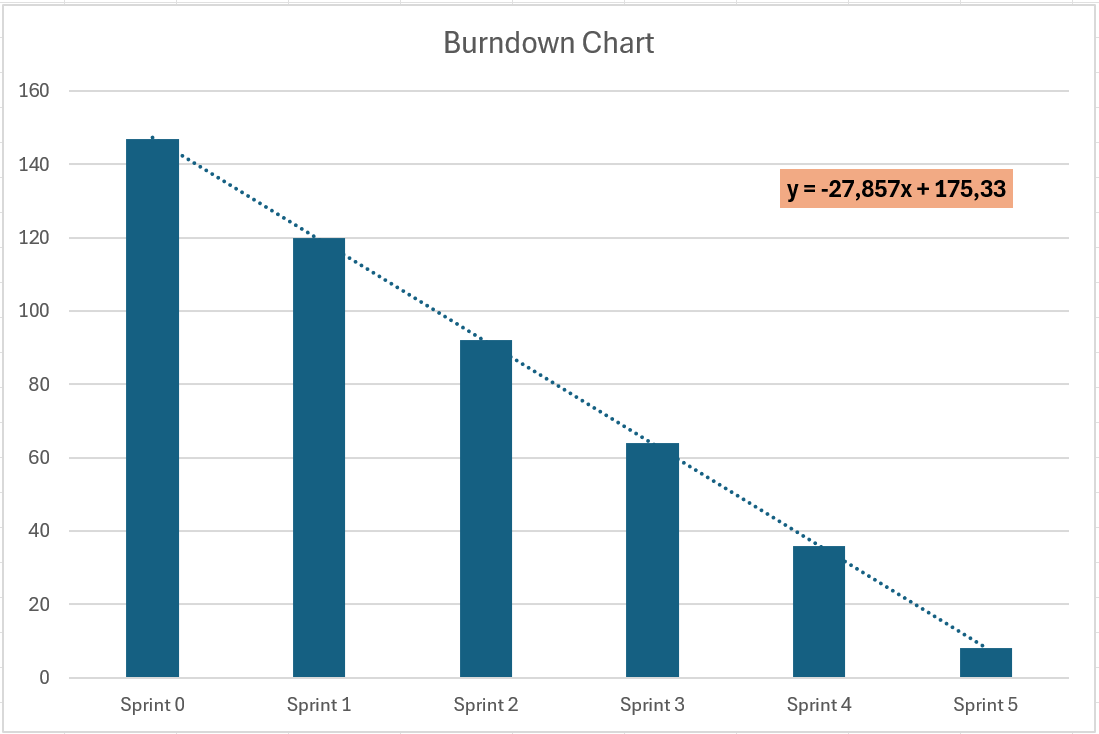
\includegraphics[width=0.8\textwidth]{figures/scrum/burndown-chart.png}
    \caption{Burndown Chart}
    \label{fig:burndown-chart}
\end{figure}

Alle \emph{sprints} blev gennemført til tiden, og alle \emph{user stories} blev gennemført til tiden. 
Der var dog en del af designet og \emph{bootstrap}, der blev nedprioriteret eller skubbet til senere \emph{sprints}, da det ikke var essentielt for den videre funktionalitet. 
Dette kan ses på \emph{Burndown Chartet} \cref{fig:burndown-chart}, hvor det er de sidste to "idé" \emph{user stories}, der ikke er blevet gennemført.
\emph{Burndown Chartet} giver en hældningskoefficient på -27,8, hvilket svarer til de ca. 28 \emph{story points}, som hvert \emph{sprint} i gennemsnit var estimeret til.

\chapter{Produktet}
\label{chapter:final-product}

\section{Programmet}
\label{sec:the-program}
Selve koden ligger offentligt tilgængelige på GitHub \cite{the-project}.

\section{Rapporten}
\label{sec:the-report}
\LaTeX til denne rapport ligger offentligt tilgængelige på GitHub \cite{the-report}.

\section{Dokumentation}
\label{sec:the-documentation}
Følger man linket \cite{the-auxiliary}, kan man finde videodemonstration af projektet, sammen med Doxygen dokumentationen for selve projektet. 

\section{Udviklerens kommentar}
\label{sec:the-developers-comment}
Projektet er blevet afsluttet til tiden, og der er blevet leveret et produkt, der opfylder de krav, der blev stillet i starten af projektet.
Der er dog nogle ting, der kunne være gjort anderledes, hvis der havde været mere tid. Designet er rudimentært men acceptabelt.
I forhold til funktionalitet, er der gået i breden fremfor dybden. Med tanke på at det er et skoleprojekt, er det dog acceptabelt, da det er vigtigere at kunne
implementere et solidt fundament af teknologier og teknikker, fremfor at enhver property og metode er suboptimeret og dokumenteret i en konsol app (subjektiv holdning).  


\chapter{Konklusion}
\label{chapter:conclusion}

\section{Opsummering}
\label{sec:conclusion_summary}

\subsection{Forretningsanalyse}
Gennem diverse modeller og analyse blev der grundlagt en solid forståelse af stakeholders egne ønsker, samt hvad projektet yderligere kunne bidrage af værdi. 
Ud fra dette skulle der udformes User Stories, som kunne bidrage til at projeket holdt kursen mod et godt produkt. 
Ydermere var der overvejet for hvilke dele og funktionaliteter, der først skulle flyttes out-of-scope, skulle der opstå modstand i løbet af processen.
Det blev vurderet at projektet var viable ud fra de stillede parametre og foranstaltninger. 

\subsection{SCRUM}
SCRUM processen blev brugt til at strukturere projektet og sikre, at der blev leveret funktionalitet til tiden.
Trello blev anvendt til at holde styr på processen og dokumentere arbejdet.
Der blev der brugt Workflows, der gav input til User Stories og Mapping. Hver User Story fik Tasks, Acceptance Criteria og et Story Point estimat.
Herfra blev der lavet en prioriteret Product Backlog, der blev brugt til at planlægge Sprints, som blev yderligere raffineret.
Gennem iterationer af Daily Standups, Sprint Reviews og Retrospectives - som var modificeret til omstændighederne - blev processen udviklet og optimeret.

\subsection{Software Design}
Der blev udarbejdet en række modeller, der beskrev systemets struktur og funktionalitet. Kernemodellerne har understøttet udviklingen af systemet og har været retningsgivende for implementeringen.
De har dog alle undergået en række ændringer i løbet af projektet, for at tilpasse sig systemets udvikling og de krav, der opstod undervejs.
Der blev lagt vægt på at designe et system, der var fleksibelt og kunne udvides med nye funktionaliteter. Bl.a. at en Employee har et Salary, der senere kan bruges i et lønsstyringsmodul.
Samtidig var brugervenlighed og det intuitive design indtænkt, så brugerne kunne finde rundt og bruge systemet uden problemer.
Hertil kom også overvejelser omkring sikkerhed og performance, der blev indtænkt i designet. Unit test blev anvendt i mindre omfang.
Den dokumentation, der blev udarbejdet, har været lavet med den hensigt, at en læser kan forstå kernedele af systemet og dets funktionalitet, uden at have været med i udviklingsprocessen.
Der er dog ikke fuld dokuemntation eller test, der beskriver alle aspekter af systemet, da det ville være for omfattende og ikke nødvendigt for projektet.
Prioriteringen er med henblik på, at have en enkelt udvikler, der har siddet med alle dele af projektet.
Der har dog været eksperimenteret med bl.a. Doxygen, for at kunne generere dokumentation.

\section{Diskussion}
\label{sec:conclusion_discussion}
Workflows fungerede ret godt, trods det opstod som en strøtanke. Prioriteringen og estimeringen af User Stories var dog mere tidskrævende end værdiskabende. 
Det kan skyldes at det var et kort og mindre omfangsrigt projekt, hvor det er nemmere at have overblik over, hvad der skal implementeres.
Sprints var en god måde at strukturere arbejdet på, da det gav en fornemmelse af, hvor meget der kunne implementeres i en uge, og dermed hvor meget der kunne implementeres i projektet som helhed.

SCRUM processen som den orginalt er beskrevet, er en fin metode med et godt værdisæt til at strukturere et projekt og sikre den rette kurs.
Den originale tanke tillader, at elementer kan skræddersys til den enkelte organisation eller projekt, og det er vigtigt at være opmærksom på, hvad der giver værdi og hvad der er spild af tid.
Dette sætter høje krav, ikke bare til at alle i teamet er bekendt med processen og er villige til at følge den, men også at teamet er samarbejdet og på bølgelængde.
Kravene til de individuelle teammedlemmer er også højere, da der kræves en vis grad af både selvstændighed og disciplin, men i den grad også kompetence og tværfaglighed for at kunne følge processen.
Underforstået, at hvis man fx som udvikler ikke har de fornødne kompetencer til at løse den øverste User Story i backloggen, så skævvrides processen og afliver tanken om "alle kan alt". 
Dette krav til kompetencer m.m. synes ikke beskrevet blandt de agile guruer. Det symptombehandles blot med mantraet om at man skal have det agile mindset, hvilket er ligeså formålstjenestligt som "Don't Panic".
Med tanke på den palette af kompetencer, der kræves, er det ikke underligt at SCRUM ofte bliver kritiseret for at være en metode, der er svær at implementere i praksis.
Ud fra egne erfaringer med at udvikle dette projekt alene, så har det stillet store krav til at kunne skifte mellem forskellige tværfaglige discipliner og teknologier. 
Alle kompetencer har været i spil og samtidig har der skulle erhverves nye eller generhverves uddaterede kompetencer, oveni at alle arbejdsopgaver kunne uddeles med et lommespejl.
Det er ikke en opgave, der er for alle, og det er ikke en opgave, der er for alle at løse alene.

Dokumentationen af systemet har været en balancegang mellem at have en forståelig og brugbar dokumentation og at have en dokumentation, der er så omfattende, at den tager for meget tid fra udviklingen.
Samtidig har der været en afvejning mellem at implementere en nye funktionalitet, afprøve den, muligvis skulle udarbejde tests og så at dokumentere den.
Det har været en udfordring at finde den rette balance, og det er ikke sikkert, at den er blevet fundet i dette projekt.  

\section{Konklusion}
\label{sec:conclusion_conclusion}
Det har været en lærerig proces, og det er klart, at der er plads til forbedring.

\section{Perspektivering}
\label{sec:conclusion_perspective}

\section{Afsluttende bemærkninger}
\label{sec:conclusion_remarks}



%% Prevent urls running into margins in bibliography
\setcounter{biburlnumpenalty}{7000}
\setcounter{biburllcpenalty}{7000}
\setcounter{biburlucpenalty}{7000}

%% Add bibliography
\printbibliography[heading=bibintoc,title={References}]

%% ----------------------------------------------------------------------
%%    Appendix (Letters for chapters)
%% ----------------------------------------------------------------------

\appendix

\chapter{User Stories}
\label{appendix:userstories}

\section{Alle User Stories}
\label{sec:all-user-stories}

\subsection{US-001 Se Alle Produkter (Kunde)}
\label{sec:US-001}
\textit{Som kunde, Ønsker jeg at se alle tilgængelige produkter, Med det formål at vælge et produkt.}
\subsubsection*{\textbf{Tasks}}
\begin{enumerate}
  \item Implementer en produktoversigtsside med alle tilgængelige produkter.
\end{enumerate}
\subsubsection*{\textbf{Acceptance Criteria}}
\begin{enumerate}
  \item Givet at en kunde besøger produktoversigtssiden, når de kigger igennem siden, så skal de kunne se alle produkter, der er til salg.
\end{enumerate}
\textbf{Estimate:} \colorbox{green}{1 (green)}
\textbf{Placed: Sprint 1}
\par\noindent\dotfill

\subsection{US-002 Oversigt over Produkter (Kunde)}
\label{sec:US-002}
\textit{Som kunde vil jeg kunne se en oversigt over blomsterarrangementer, så jeg kan vælge det, der passer til lejligheden.}
\subsubsection*{\textbf{Tasks}}
\begin{enumerate}
  \item Implementer kategorier, hvor produkter der har samme tema vises
\end{enumerate}
\subsubsection*{\textbf{Acceptance Criteria}}
\begin{enumerate}
  \item Givet at en kunde vil se en bestemt produktkategori, når de leder efter et produkt der opfylder deres behov, så får de en tilsvarende afgrænset visning af produktkataloget.
\end{enumerate}
\textbf{Estimate:} \colorbox{yellow}{3 (yellow)}
\textbf{Placed: Sprint 1}
\par\noindent\dotfill

\subsection{US-003 Tilføj til Kurv (Kunde)}
\label{sec:US-003}
\textit{Som kunde, Ønsker jeg at tilføje et produkt til min kurv, Med det formål at samle min bestilling.}
\subsubsection*{\textbf{Tasks}}
\begin{enumerate}
  \item Implementer en funktion til at tilføje produkter til en indkøbskurv.
\end{enumerate}
\subsubsection*{\textbf{Acceptance Criteria}}
\begin{enumerate}
  \item Givet at en kunde vælger et produkt, når de klikker på 'tilføj til kurv'-knappen, så skal produktet blive tilføjet til deres kurv.
\end{enumerate}
\textbf{Estimate:} \colorbox{orange}{5 (orange)}
\textbf{Placed: Sprint 1}
\par\noindent\dotfill

\subsection{US-004 Ændre Produkter i Kurv (Bruger)}
\label{sec:US-004}
\textit{Som bruger, Ønsker jeg at ændre mængden af produkter i min kurv, Med det formål at justere min bestilling før køb.}
\subsubsection*{\textbf{Tasks}}
\begin{enumerate}
  \item Implementer en redigeringsfunktion i kurven, hvor brugeren kan opdatere antallet eller fjerne produkter fra kurven.
\end{enumerate}
\subsubsection*{\textbf{Acceptance Criteria}}
\begin{enumerate}
  \item Givet at en bruger ønsker at ændre sin bestilling, når de besøger kurvsiden, så skal de kunne ændre antallet af produkter eller fjerne dem fra kurven.
\end{enumerate}
\textbf{Estimate:} \colorbox{lime}{2 (lime)}
\textbf{Placed: Sprint 1}
\par\noindent\dotfill

\subsection{US-005 Opret Ordre (Kunde)}
\label{sec:US-005}
\textit{Som kunde, Ønsker jeg at skabe en ordre fra min kurv, Med det formål at købe de valgte produkter.}
\subsubsection*{\textbf{Tasks}}
\begin{enumerate}
  \item Udvikle en proces, hvor kunden kan omdanne indholdet af kurven til en ordre.
\end{enumerate}
\subsubsection*{\textbf{Acceptance Criteria}}
\begin{enumerate}
  \item Givet at en kunde har valgt produkter i kurven, når de klikker på 'bestil', så skal de kunne gennemføre købet og se en ordrebekræftelse.
\end{enumerate}
\textbf{Estimate:} \colorbox{lime}{2 (lime)}
\textbf{Placed: Sprint 1}
\par\noindent\dotfill

\subsection{US-006 Kurv til Ordre}
\label{sec:US-006}
\textit{Som ejer, Ønsker jeg at kunden skal give relevant kontaktinformation for at kunne købe en ordre fra kurven, Med det formål at undgå anonyme køb.}
\subsubsection*{\textbf{Tasks}}
\begin{enumerate}
  \item Kræv at brugere afgiver kontaktinformation, uden at oprette bruger
\end{enumerate}
\subsubsection*{\textbf{Acceptance Criteria}}
\begin{enumerate}
  \item Givet at en anonym kunde ønsker at købe produkterne i kurv, når de forsøger at gøre dette, så bliver de bedt om at logge ind, oprette en konto eller afgive kontaktinformation.
\end{enumerate}
\textbf{Estimate:} \colorbox{yellow}{3 (yellow)}
\textbf{Placed: Sprint 1}
\par\noindent\dotfill

\subsection{US-007 Registrerer sig (Kunde)}
\label{sec:US-007}
\textit{Som kunde, ønsker jeg selv at kunne registrer mig til webshoppen, så jeg hurtigst muligt kan udnytte fordele ved at være registreret bruger}
\subsubsection*{\textbf{Tasks}}
\begin{enumerate}
  \item Implementer registrerings funktion
  \item Opret registreringsside
\end{enumerate}
\subsubsection*{\textbf{Acceptance Criteria}}
\begin{enumerate}
  \item Givet at en anonym bruger, når denne vil registrerer sig på sitet, så vil denne få en bruger, som vedkommende kan logge ind med
\end{enumerate}
\textbf{Estimate:} \colorbox{orange}{5 (orange)}
\textbf{Placed: Sprint 1}
\par\noindent\dotfill

\subsection{US-008 Log ind (Kunde)}
\label{sec:US-008}
\textit{Som kunde vil jeg kunne logge ind, så jeg kan se mine ordrer og betalinger.}
\subsubsection*{\textbf{Tasks}}
\begin{enumerate}
  \item Implementer login funktion
  \item Implementer 'forkert password' funktion
\end{enumerate}
\subsubsection*{\textbf{Acceptance Criteria}}
\begin{enumerate}
  \item Givet at en registreret kunde ønsker at logge ind når denne ønsker at interagere med siden som en registreret bruger, så vil denne logge ind, såfremt korrekt password og username er anvendt
\end{enumerate}
\textbf{Estimate:} \colorbox{yellow}{3 (yellow)}
\textbf{Placed: Sprint 1}
\par\noindent\dotfill

\subsection{US-009 Log ud (Kunde)}
\label{sec:US-009}
\textit{Som kunde vil jeg kunne logge ud, så jeg kan sikre, at mine oplysninger ikke er tilgængelige for andre.}
\subsubsection*{\textbf{Tasks}}
\begin{enumerate}
  \item Implementer log ud funktion
  \item Implementer auto-log ud funktion
\end{enumerate}
\subsubsection*{\textbf{Acceptance Criteria}}
\begin{enumerate}
  \item Givet at en kunde vil logge ud, når denne er færdig med at interagere med sitet, så vil denne logges ud og returneres til forsiden
\end{enumerate}
\textbf{Estimate:} \colorbox{yellow}{3 (yellow)}
\textbf{Placed: Sprint 1}
\par\noindent\dotfill

\subsection{US-010 Profiloplysninger (Kunde)}
\label{sec:US-010}
\textit{Som kunde vil jeg kunne se en oversigt over mine personlige oplysninger, så jeg kan se, hvad I har registreret om mig.}
\subsubsection*{\textbf{Acceptance Criteria}}
\begin{enumerate}
  \item Givet at en kunde vil se sine egne registrerede oplysninger, når kunden er på sin profilside, så vil kunden kunne se dem på en heuristisk designet facon
\end{enumerate}
\subsubsection*{\textbf{Tasks}}
\begin{enumerate}
  \item Opret side, hvor den kunde, der er logget ind, kan se sine egne oplysninger
\end{enumerate}
\textbf{Estimate:} \colorbox{yellow}{3 (yellow)}
\textbf{Placed: Sprint 2}
\par\noindent\dotfill

\subsection{US-011 Ændre profiloplysninger (Kunde)}
\label{sec:US-011}
\textit{Som kunde vil jeg kunne ændre mine personlige oplysninger, så jeg kan sikre, at de er korrekte.}
\subsubsection*{\textbf{Tasks}}
\begin{enumerate}
  \item Kunde skal kunne ændre i egen personlige oplysninger
\end{enumerate}
\subsubsection*{\textbf{Acceptance Criteria}}
\begin{enumerate}
  \item Givet at en kunde vil opdatere sine oplysninger, når disse har ændret sig, så vil kunden kunne se sine oplysninger er opdateret til det af kunden angivne værdier
\end{enumerate}
\textbf{Estimate:} \colorbox{yellow}{3 (yellow)}
\textbf{Placed: Sprint 2}
\par\noindent\dotfill

\subsection{US-012 Log Ind på Ordreportal (Medarbejder)}
\label{sec:US-012}
\textit{Som medarbejder, Ønsker jeg at kunne logge ind på ordreportalen, Med det formål at kunne ekspedere ordrer.}
\subsubsection*{\textbf{Acceptance Criteria}}
\begin{enumerate}
  \item Givet at en medarbejder står foran sin arbejdsstation, når de indtaster deres legitimationsoplysninger, så skal de have adgang til ordreportalen, hvor de kan administrere ordrer.
\end{enumerate}
\subsubsection*{\textbf{Tasks}}
\begin{enumerate}
  \item Implementer en sikker log ind-funktion specifikt for medarbejdere på ordreportalen.
\end{enumerate}
\textbf{Estimate:} \colorbox{orange}{5 (orange)}
\textbf{Placed: Sprint 2}
\par\noindent\dotfill

\subsection{US-013 Produktadministration (Bestyrer)}
\label{sec:US-013}
\textit{Som bestyrer, Ønsker jeg at kunne oprette og opdatere produkter i webshoppen, Med det formål at sikre, at produktudvalget altid er aktuelt og korrekt prissat.}
\subsubsection*{\textbf{Tasks}}
\begin{enumerate}
  \item Udvikle en brugergrænseflade for produktadministration i administrationspanelet.
  \item Implementere et samlet dashboard med oversigt over alle Produkter
\end{enumerate}
\subsubsection*{\textbf{Acceptance Criteria}}
\begin{enumerate}
  \item Givet at en bestyrer er logget ind, når de tilgår produktadministrationsmodulet, så skal de kunne tilføje nye produkter, redigere eksisterende produkter og arkivere forældede produkter.
\end{enumerate}
\textbf{Estimate:} \colorbox{orange}{5 (orange)}
\textbf{Placed: Sprint 2}
\par\noindent\dotfill

\subsection{US-014 Ordreoversigt (Medarbejder)}
\label{sec:US-014}
\textit{Som medarbejder, Ønsker jeg at kunne se alle ordrer, Med det formål at få et overblik over arbejdsbyrden.}
\subsubsection*{\textbf{Tasks}}
\begin{enumerate}
  \item Udvikle et dashboard, hvor medarbejdere kan se en liste over alle aktuelle ordrer.
\end{enumerate}
\subsubsection*{\textbf{Acceptance Criteria}}
\begin{enumerate}
  \item Givet at en medarbejder er logget ind, når de tilgår dashboardet, så skal de kunne se og sortere alle ordrer efter status, dato og andre relevante kriterier.
\end{enumerate}
\textbf{Estimate:} \colorbox{yellow}{3 (yellow)}
\textbf{Placed: Sprint 2}
\par\noindent\dotfill

\subsection{US-015 Ordrehåndtering (Medarbejder)}
\label{sec:US-015}
\textit{Som medarbejder, Ønsker jeg at kunne se og administrere indkommende ordrer, Med det formål at effektivisere processen for ordreklargøring og levering.}
\subsubsection*{\textbf{Tasks}}
\begin{enumerate}
  \item Implementer en administrationsside for medarbejdere til håndtering af nye ordrer.
\end{enumerate}
\subsubsection*{\textbf{Acceptance Criteria}}
\begin{enumerate}
  \item Givet at en medarbejder er logget ind, når de tilgår administrationspanelet, så skal de kunne se en liste over aktive ordrer og opdatere deres status.
\end{enumerate}
\textbf{Estimate:} \colorbox{yellow}{3 (yellow)}
\textbf{Placed: Sprint 2}
\par\noindent\dotfill

\subsection{US-016 Opdatere Ordrestatus (Medarbejder)}
\label{sec:US-016}
\textit{Som medarbejder, Ønsker jeg at kunne opdatere ordrestatus, Med det formål at tydeliggøre for alle brugere, hvor langt ordren er i processen.}
\subsubsection*{\textbf{Tasks}}
\begin{enumerate}
  \item Skabe en funktion, der tillader medarbejdere at opdatere status for en ordre i realtid.
\end{enumerate}
\subsubsection*{\textbf{Acceptance Criteria}}
\begin{enumerate}
  \item Givet at en ordre er i gang med at blive ekspederet, når medarbejderen opdaterer ordrens status, så skal denne opdatering være synlig for alle relevante parter, herunder andre medarbejdere og kunden, hvis de tjekker status online.
\end{enumerate}
\textbf{Estimate:} \colorbox{yellow}{3 (yellow)}
\textbf{Placed: Sprint 2}
\par\noindent\dotfill

\subsection{US-017 Se Ordredetaljer (Medarbejder)}
\label{sec:US-017}
\textit{Som medarbejder, Ønsker jeg at kunne se ordredetaljer om blomsterarrangementet, Med det formål at kunne ekspedere ordrer korrekt og effektivt.}
\subsubsection*{\textbf{Tasks}}
\begin{enumerate}
  \item Udvikle en funktion, der viser fulde detaljer for hver ordre, inklusive specifikationer for blomsterarrangementet.
\end{enumerate}
\subsubsection*{\textbf{Acceptance Criteria}}
\begin{enumerate}
  \item Givet at en medarbejder behandler en ordre, når de tilgår ordren på systemet, så skal de kunne se alle relevante detaljer om blomsterarrangementet, som er nødvendige for at færdiggøre ordren korrekt.
\end{enumerate}
\textbf{Estimate:} \colorbox{green}{1 (green)}
\textbf{Placed: Sprint 2}
\par\noindent\dotfill

\subsection{US-018 Ordreklargøring (Medarbejder)}
\label{sec:US-018}
\textit{Som medarbejder, Ønsker jeg at markere en ordre som klar til afhentning og fuldført, Med det formål at administrere ordreflowet effektivt.}
\subsubsection*{\textbf{Tasks}}
\begin{enumerate}
  \item Skab en funktion, hvor medarbejdere kan opdatere ordrens status til 'klar til afhentning' og senere 'afhentet'.
\end{enumerate}
\subsubsection*{\textbf{Acceptance Criteria}}
\begin{enumerate}
  \item Givet at en ordre er færdigpakket, når medarbejderen opdaterer systemet, så skal statussen ændres, så kunden og andre medarbejdere kan se, at ordren er klar eller afhentet.
\end{enumerate}
\textbf{Estimate:} \colorbox{lime}{2 (lime)}
\textbf{Placed: Sprint 2}
\par\noindent\dotfill

\subsection{US-019 Ordreansvar (Medarbejder)}
\label{sec:US-019}
\textit{Som medarbejder, Ønsker jeg at kunne tildele en ordre til mig selv, Med det formål at sikre ansvarsfordelingen for ordrehåndteringen.}
\subsubsection*{\textbf{Tasks}}
\begin{enumerate}
  \item Udvikle et system, hvor medarbejdere kan tildele specifikke ordrer til sig selv for håndtering.
\end{enumerate}
\subsubsection*{\textbf{Acceptance Criteria}}
\begin{enumerate}
  \item Givet at en ordre skal behandles, når en medarbejder vælger ordren, så skal de kunne markere den som 'under behandling' af sig selv.
\end{enumerate}
\textbf{Estimate:} \colorbox{lime}{2 (lime)}
\textbf{Placed: Sprint 3}
\par\noindent\dotfill

\subsection{US-020 Ordrefilter og -sortering (Medarbejder)}
\label{sec:US-020}
\textit{Som medarbejder, Ønsker jeg at filtrere og sortere ordrer, Med det formål at få et overblik over ordrer, der er forfaldne eller som jeg er ansvarlig for.}
\subsubsection*{\textbf{Acceptance Criteria}}
\begin{enumerate}
  \item Givet at der er behov for at organisere ordrer, når medarbejderen anvender filter og sorteringsfunktionerne, så skal de kunne se en organiseret liste over ordrer.
\end{enumerate}
\subsubsection*{\textbf{Tasks}}
\begin{enumerate}
  \item Implementere filter og sorteringsfunktioner i ordreoversigten.
\end{enumerate}
\textbf{Estimate:} \colorbox{yellow}{3 (yellow)}
\textbf{Placed: Sprint 3}
\par\noindent\dotfill

\subsection{US-021 Speciel Ordre Funktion (Bedemand)}
\label{sec:US-021}
\textit{Som bedemand, Ønsker jeg at kunne bestille specialdesignet blomsterarrangement direkte via en dedikeret side, Med det formål at effektivisere bestillingsprocessen for begravelsesarrangementer.}
\subsubsection*{\textbf{Acceptance Criteria}}
\begin{enumerate}
  \item Givet at en bedemand er logget ind, når de tilgår den dedikerede side, så skal de kunne vælge og tilpasse blomsterarrangementer specielt designet til begravelser.
\end{enumerate}
\subsubsection*{\textbf{Tasks}}
\begin{enumerate}
  \item Opret en dedikeret side for bedemænd med tilpassede bestillingsmuligheder.
\end{enumerate}
\textbf{Estimate:} \colorbox{yellow}{3 (yellow)}
\textbf{Placed: Sprint 3}
\par\noindent\dotfill

\subsection{US-022 Produktfiltrering (Kunde)}
\label{sec:US-022}
\textit{Som kunde, Ønsker jeg at kunne filtrere produkter på produktsiden, Med det formål nemt at finde det rigtige produkt.}
\subsubsection*{\textbf{Acceptance Criteria}}
\begin{enumerate}
  \item Givet at en kunde søger efter et specifikt produkt, når de bruger filterfunktionerne, så skal de kunne se en filtreret liste af produkter, der matcher deres kriterier.
\end{enumerate}
\subsubsection*{\textbf{Tasks}}
\begin{enumerate}
  \item Oprette filter og sorteringsfunktioner i ordreoversigten.
\end{enumerate}
\textbf{Estimate:} \colorbox{yellow}{3 (yellow)}
\textbf{Placed: Sprint 3}
\par\noindent\dotfill

\subsection{US-023 Navigation i Profil (Kunde)}
\label{sec:US-023}
\textit{Som kunde, Ønsker jeg at kunne navigere nemt på mine profilsider, Med det formål at brugeroplevelsen føles glidende og uforstyrret.}
\subsubsection*{\textbf{Acceptance Criteria}}
\begin{enumerate}
  \item Givet at en kunde ønsker at administrere sin profil, når de navigerer på deres profil, så skal de kunne gøre det uden forvirring eller forstyrrelser.
\end{enumerate}
\subsubsection*{\textbf{Tasks}}
\begin{enumerate}
  \item Design en brugervenlig og intuitiv grænseflade for kundens profilområde.
\end{enumerate}
\textbf{Estimate:} \colorbox{yellow}{3 (yellow)}
\textbf{Placed: Sprint 3}
\par\noindent\dotfill

\subsection{US-024 Ordreopfølgning (Kunde)}
\label{sec:US-024}
\textit{Som kunde, Ønsker jeg at kunne spore status for min ordre, Med det formål at holde mig opdateret om leveringstidspunktet.}
\subsubsection*{\textbf{Tasks}}
\begin{enumerate}
  \item Implementer en funktion til ordreopfølgning på kundens profilside.
  \item Dashboard til kunden, så de kan se alle deres ordre
\end{enumerate}
\subsubsection*{\textbf{Acceptance Criteria}}
\begin{enumerate}
  \item Givet at kunden har afgivet en ordre, når de logger ind og tjekker deres ordrestatus, så skal de kunne se den aktuelle status og forventet leveringstidspunkt.
\end{enumerate}
\textbf{Estimate:} \colorbox{yellow}{3 (yellow)}
\textbf{Placed: Sprint 3}
\par\noindent\dotfill

\subsection{US-025 Opret Nyt Produkt (Medarbejder/Administrator)}
\label{sec:US-025}
\textit{Som medarbejder/administrator, Ønsker jeg at kunne oprette et nyt produkt, Med det formål at holde produktkataloget opdateret med nye varer.}
\subsubsection*{\textbf{Acceptance Criteria}}
\begin{enumerate}
  \item Givet at webshoppen skal have nye produkter tilføjet, når medarbejder/administrator indtaster produktdetaljerne og uploader billeder, så skal det nye produkt være tilgængeligt i webshoppen.
\end{enumerate}
\subsubsection*{\textbf{Tasks}}
\begin{enumerate}
  \item Skabe en tilføj produkt-funktion på webshoppen for medarbejdere og administratorer.
\end{enumerate}
\textbf{Estimate:} \colorbox{yellow}{3 (yellow)}
\textbf{Placed: Sprint 3}
\par\noindent\dotfill

\subsection{US-026 Produktopdatering (Medarbejder)}
\label{sec:US-026}
\textit{Som medarbejder, Ønsker jeg at opdatere produkter, Med det formål at styre lagerbeholdningen.}
\subsubsection*{\textbf{Tasks}}
\begin{enumerate}
  \item Udvikle et interface til opdatering af produktinformationer og lagerstatus.
\end{enumerate}
\subsubsection*{\textbf{Acceptance Criteria}}
\begin{enumerate}
  \item Givet at et produkt behøver en opdatering, når medarbejderen ændrer informationen i systemet, så skal disse ændringer være synlige på webshoppen.
\end{enumerate}
\textbf{Estimate:} \colorbox{yellow}{3 (yellow)}
\textbf{Placed: Sprint 3}
\par\noindent\dotfill

\subsection{US-027 Deaktiver Produkt (Medarbejder/Administrator)}
\label{sec:US-027}
\textit{Som medarbejder/administrator, Ønsker jeg at kunne deaktivere et produkt, Med det formål at fjerne gamle produkter fra produktkataloget.}
\subsubsection*{\textbf{Tasks}}
\begin{enumerate}
  \item Implementer en funktion til at deaktivere produkter i produktoversigten.
\end{enumerate}
\subsubsection*{\textbf{Acceptance Criteria}}
\begin{enumerate}
  \item Givet at et produkt ikke længere skal sælges, når medarbejder/administrator deaktiverer produktet i systemet, så skal produktet ikke længere være synligt for kunder.
\end{enumerate}
\textbf{Estimate:} \colorbox{orange}{5 (orange)}
\textbf{Placed: Sprint 3}
\par\noindent\dotfill

\subsection{US-028 Genskabe Produkt (Medarbejder)}
\label{sec:US-028}
\textit{Som medarbejder, Ønsker jeg at kunne se deaktiverede produkter og genaktivere dem, Med det formål at administrere produktkataloget.}
\subsubsection*{\textbf{Tasks}}
\begin{enumerate}
  \item Tilføje en funktion til at se og reaktivere deaktiverede produkter.
\end{enumerate}
\subsubsection*{\textbf{Acceptance Criteria}}
\begin{enumerate}
  \item Givet at et produkt tidligere er blevet deaktiveret, når medarbejderen ønsker at genaktivere det, så skal produktet igen kunne vises og sælges på hjemmesiden.
\end{enumerate}
\textbf{Estimate:} \colorbox{orange}{5 (orange)}
\textbf{Placed: Sprint 4}
\par\noindent\dotfill

\subsection{US-029 Leveringsvalg (Bedemand)}
\label{sec:US-029}
\textit{Som bedemand, Ønsker jeg at kunne vælge leveringssted og -tid, Med det formål at kunne drive min forretning.}
\subsubsection*{\textbf{Tasks}}
\begin{enumerate}
  \item Skabe et brugerinterface, hvor bedemænd kan vælge leveringsdetaljer ved bestilling.
\end{enumerate}
\subsubsection*{\textbf{Acceptance Criteria}}
\begin{enumerate}
  \item Givet at en bedemand laver en bestilling, når de indtaster leveringsoplysninger, så skal disse oplysninger anvendes til ordren.
\end{enumerate}
\textbf{Estimate:} \colorbox{orange}{5 (orange)}
\textbf{Placed: Sprint 4}
\par\noindent\dotfill

\subsection{US-030 Tekstsøgning efter Produkter (Kunde)}
\label{sec:US-030}
\textit{Som kunde, Ønsker jeg at søge efter produkter med tekst, Med det formål at hurtigt finde, hvad jeg har i tankerne.}
\subsubsection*{\textbf{Tasks}}
\begin{enumerate}
  \item Integrer en søgefunktion i webshoppen, som tillader tekstbaseret søgning.
\end{enumerate}
\subsubsection*{\textbf{Acceptance Criteria}}
\begin{enumerate}
  \item Givet at en kunde ved, hvad de leder efter, når de indtaster søgekriterier, så skal de præsenteres for relevante produktresultater.
\end{enumerate}
\textbf{Estimate:} \colorbox{red}{8 (red)}
\textbf{Placed: Sprint 4}
\par\noindent\dotfill

\subsection{US-031 Visning af Søgeresultater (Bruger)}
\label{sec:US-031}
\textit{Som bruger, Ønsker jeg at kunne se mine søgeresultater, Med det formål at kunne vælge et produkt fra resultaterne.}
\subsubsection*{\textbf{Tasks}}
\begin{enumerate}
  \item Skabe en visning, der effektivt præsenterer resultaterne af en produktsøgning.
\end{enumerate}
\subsubsection*{\textbf{Acceptance Criteria}}
\begin{enumerate}
  \item Givet at en bruger har foretaget en søgning, når søgeresultaterne vises, så skal de være klare og lette at navigere i.
\end{enumerate}
\textbf{Estimate:} \colorbox{lime}{2 (lime)}
\textbf{Placed: Sprint 4}
\par\noindent\dotfill

\subsection{US-032 Sortering og Filtrering af Søgeresultater (Bruger)}
\label{sec:US-032}
\textit{Som bruger, Ønsker jeg at kunne sortere og filtrere søgeresultaterne efter en produktsøgning, Med det formål bedre at finde det, jeg leder efter.}
\subsubsection*{\textbf{Tasks}}
\begin{enumerate}
  \item Tilføj sortering og filtreringsmuligheder til søgeresultatsiden. Bl.a. Fritekst søgning.
\end{enumerate}
\subsubsection*{\textbf{Acceptance Criteria}}
\begin{enumerate}
  \item Givet at en bruger har udført en søgning og ser på resultaterne, når de anvender filtrerings og sorteringsfunktionerne, så skal listen over produkter opdatere sig i henhold til de valgte kriterier.
\end{enumerate}
\textbf{Estimate:} \colorbox{red}{8 (red)}
\textbf{Placed: Sprint 4}
\par\noindent\dotfill

\subsection{US-033 Kurvindikator (Kunde)}
\label{sec:US-033}
\textit{Som kunde, Ønsker jeg at se antallet af produkter i min kurv uden at være på kurvsiden, Med det formål at kunne holde styr på mine valgte varer med lethed.}
\subsubsection*{\textbf{Tasks}}
\begin{enumerate}
  \item Tilføj en indikator på hjemmesiden, der viser antal produkter i kurven.
\end{enumerate}
\subsubsection*{\textbf{Acceptance Criteria}}
\begin{enumerate}
  \item Givet at en kunde har tilføjet produkter til deres kurv, når de navigerer væk fra kurvsiden, så skal de stadig kunne se en indikator med antal produkter i kurven.
\end{enumerate}
\textbf{Estimate:} \colorbox{yellow}{3 (yellow)}
\textbf{Placed: Sprint 5}
\par\noindent\dotfill

\subsection{US-034 Automatiske notifikationer (Medarbejder)}
\label{sec:US-034}
\textit{Som medarbejder, Ønsker jeg at modtage automatiske notifikationer om nye ordrer, Med det formål at kunne påbegynde ordrebehandling så hurtigt som muligt.}
\subsubsection*{\textbf{Tasks}}
\begin{enumerate}
  \item Implementer en notifikationsfunktion, der alarmerer medarbejdere om nye ordrer via e-mail eller systempopup.
\end{enumerate}
\subsubsection*{\textbf{Acceptance Criteria}}
\begin{enumerate}
  \item Givet at en ny ordre er afgivet, når ordren registreres i systemet, så modtager relevante medarbejdere en notifikation.
\end{enumerate}
\textbf{Estimate:} \colorbox{orange}{5 (orange)}
\textbf{Placed: Sprint 5}
\par\noindent\dotfill

\subsection{US-035 Salgsrapporter (Bestyrer)}
\label{sec:US-035}
\textit{Som bestyrer, Ønsker jeg at kunne generere detaljerede salgsrapporter, Med det formål at analysere salgstendenser og foretage datadrevne beslutninger.}
\subsubsection*{\textbf{Tasks}}
\begin{enumerate}
  \item Udvikle en funktion til at generere og eksportere salgsrapporter i administrationspanelet.
\end{enumerate}
\subsubsection*{\textbf{Acceptance Criteria}}
\begin{enumerate}
  \item Givet at en bestyrer ønsker at se salgsdata, når de vælger rapporteringsperioden og genererer rapporten, så præsenteres de for en detaljeret rapport over salg fordelt på produkter, kategorier og tidspunkter.
\end{enumerate}
\textbf{Estimate:} \colorbox{red}{8 (red)}
\textbf{Placed: Sprint 5}
\par\noindent\dotfill

\subsection{US-036 Automatisk Fakturering (Bedemand)}
\label{sec:US-036}
\textit{Som bedemand, Ønsker jeg automatisk at modtage en faktura ved bestilling, Med det formål at forenkle regnskabsprocessen.}
\subsubsection*{\textbf{Tasks}}
\begin{enumerate}
  \item Udvikle en automatisk faktureringsproces, der sender fakturaer direkte til bedemandens e-mail efter ordreafgivelse.
\end{enumerate}
\subsubsection*{\textbf{Acceptance Criteria}}
\begin{enumerate}
  \item Givet at en bedemand afgiver en bestilling, når ordren er bekræftet, så modtager de en faktura via e-mail.
\end{enumerate}
\textbf{Estimate:} \colorbox{orange}{5 (orange)}
\textbf{Placed: Sprint 5}
\par\noindent\dotfill

\subsection{US-037 Slet Bruger (Admin)}
\label{sec:US-037}
\textit{Som administrator, Ønsker jeg at kunne slette en bruger, Med det formål at kunne administrere medarbejdere, bedemænd og kunder.}
\subsubsection*{\textbf{Tasks}}
\begin{enumerate}
  \item Implementer en slet-funktion i adminpanelet for brugere. Denne må ikke Cascade slette, så Ordre bliver slettet.
\end{enumerate}
\subsubsection*{\textbf{Acceptance Criteria}}
\begin{enumerate}
  \item Givet at en bruger ikke længere skal have adgang til systemet, når administratoren sletter brugeren, så skal brugerens konto ikke længere være aktiv eller tilgængelig.
\end{enumerate}
\textbf{Estimate:} \colorbox{lime}{2 (lime)}
\textbf{Placed: Sprint 5}
\par\noindent\dotfill

\subsection{US-038 Slette personlige oplysninger (Kunde)}
\label{sec:US-038}
\textit{Som kunde vil jeg kunne slette mine personlige oplysninger, så jeg kan sikre, at de ikke længere er tilgængelige.}
\subsubsection*{\textbf{Acceptance Criteria}}
\begin{enumerate}
  \item Givet at en en kunde vil slette sine oplysninger, når kunden ønsker det, så bliver de berørte oplysninger slettet, men uden at påvirke bl.a. butikkens regnskabspligt
\end{enumerate}
\subsubsection*{\textbf{Tasks}}
\begin{enumerate}
  \item Oprette funktion, hvor kundens oplysninger bliver slettet
  \item Bevar en GUID, så butikkens oversigt over ordre ikke bliver påvirket
\end{enumerate}
\textbf{Estimate:} \colorbox{orange}{5 (orange)}
\textbf{Placed: Sprint 5}
\par\noindent\dotfill

\subsection{US-039 US X Template ()}
\label{sec:US-039}
\textit{}
\subsubsection*{\textbf{Tasks}}
\begin{enumerate}
\end{enumerate}
\subsubsection*{\textbf{Acceptance Criteria}}
\begin{enumerate}
\end{enumerate}
\textbf{Estimate:} \colorbox{orange}{5 (orange)}
\textbf{Placed: Project Ideas}
\par\noindent\dotfill

\subsection{US-040 Feedback og anmeldelser (Kunde)}
\label{sec:US-040}
\textit{Som kunde, Ønsker jeg at kunne afgive feedback og anmelde produkter, Med det formål at dele min oplevelse med andre kunder og hjælpe dem med at træffe informerede købsbeslutninger.}
\subsubsection*{\textbf{Tasks}}
\begin{enumerate}
  \item Implementer en feedback og anmeldelsesfunktion på produkt siderne.
\end{enumerate}
\subsubsection*{\textbf{Acceptance Criteria}}
\begin{enumerate}
  \item Givet at en kunde har købt et produkt, når de besøger produktets side efter købet, så skal de kunne skrive og indsende en anmeldelse.
\end{enumerate}
\textbf{Estimate:} \colorbox{yellow}{3 (yellow)}
\textbf{Placed: Project Ideas}
\par\noindent\dotfill

\subsection{US-041 Gavekort og rabatkoder (Kunde)}
\label{sec:US-041}
\textit{Som kunde, Ønsker jeg at kunne anvende gavekort og rabatkoder ved checkout, Med det formål at udnytte tilbud og spare penge på køb.}
\subsubsection*{\textbf{Acceptance Criteria}}
\begin{enumerate}
  \item Givet at en kunde har et gyldigt gavekort eller rabatkode, når de indtaster koden ved checkout, så skal den pågældende rabat eller gavekortets værdi fratrækkes fra den samlede ordre.
\end{enumerate}
\subsubsection*{\textbf{Tasks}}
\begin{enumerate}
  \item Udvikle en funktion, der tillader kunder at indløse gavekort og anvende rabatkoder ved betaling.
\end{enumerate}
\textbf{Estimate:} \colorbox{orange}{5 (orange)}
\textbf{Placed: Project Ideas}
\par\noindent\dotfill
\chapter{Diagrammer}
\label{appendix:diagrams}

\section{Domænemodel}
\label{appendix:domain-model-diagram}

\begin{figure}
    \centering
    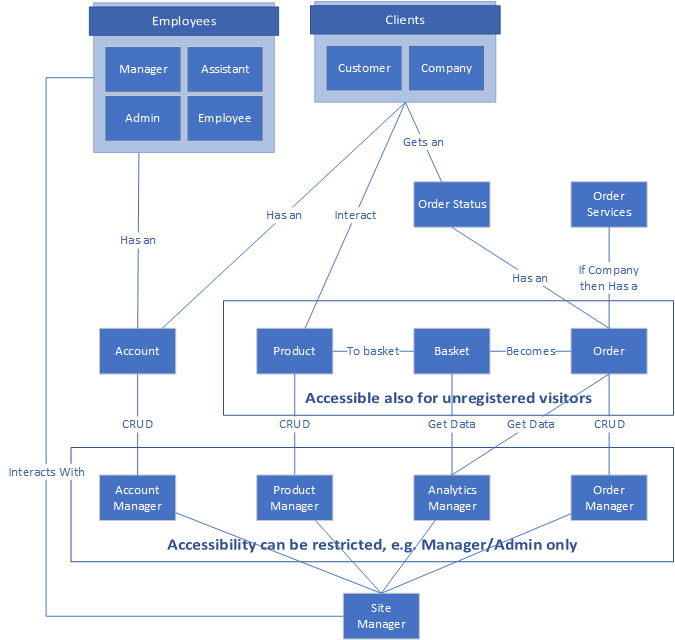
\includegraphics[width=1\textwidth]{figures/diagrams/dmd-start.png}
    \caption{Domain Model Diagram ved projektets start}
    \label{fig:appendix-domain-model-diagram}
\end{figure}

\section{Designklassediagrammer}
\label{appendix:class-diagrams}

\begin{figure}
    \centering
    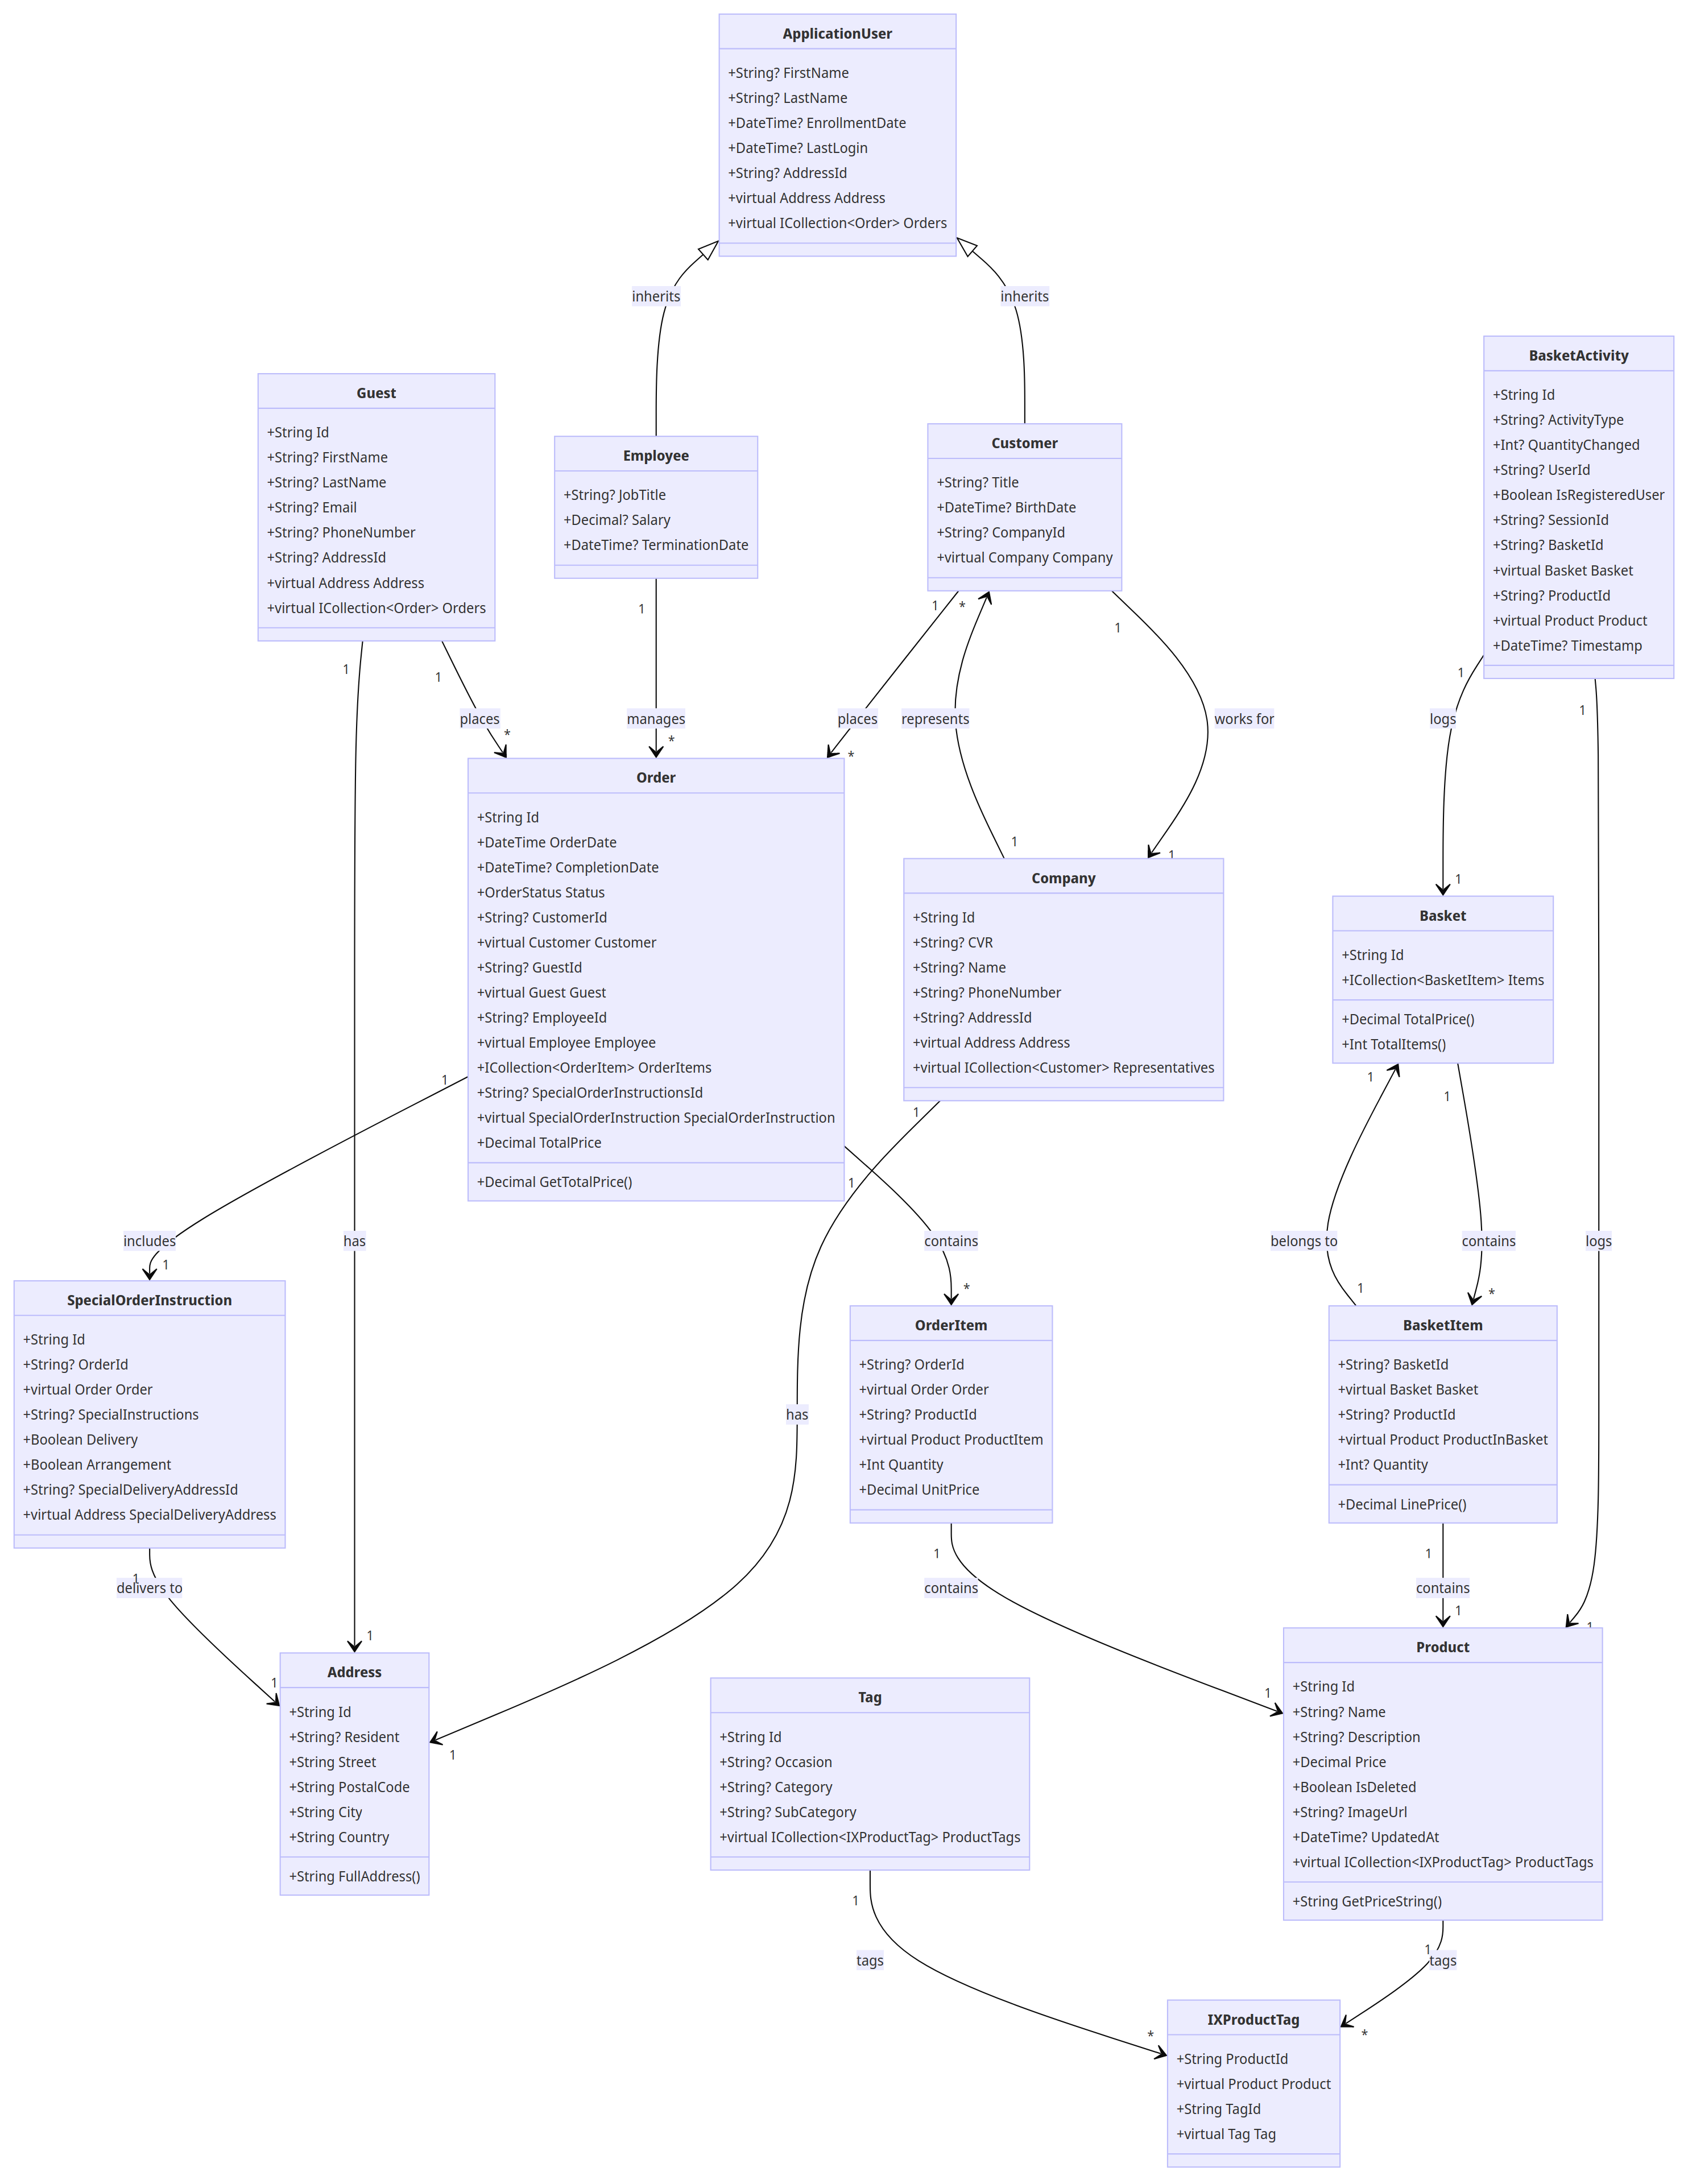
\includegraphics[width=1\textwidth]{figures/diagrams/dcd-modelclasses.png}
    \caption{Design Class Diagram - Model Classes}
    \label{fig:class-diagram-models}
\end{figure}

\begin{figure}
    \centering
    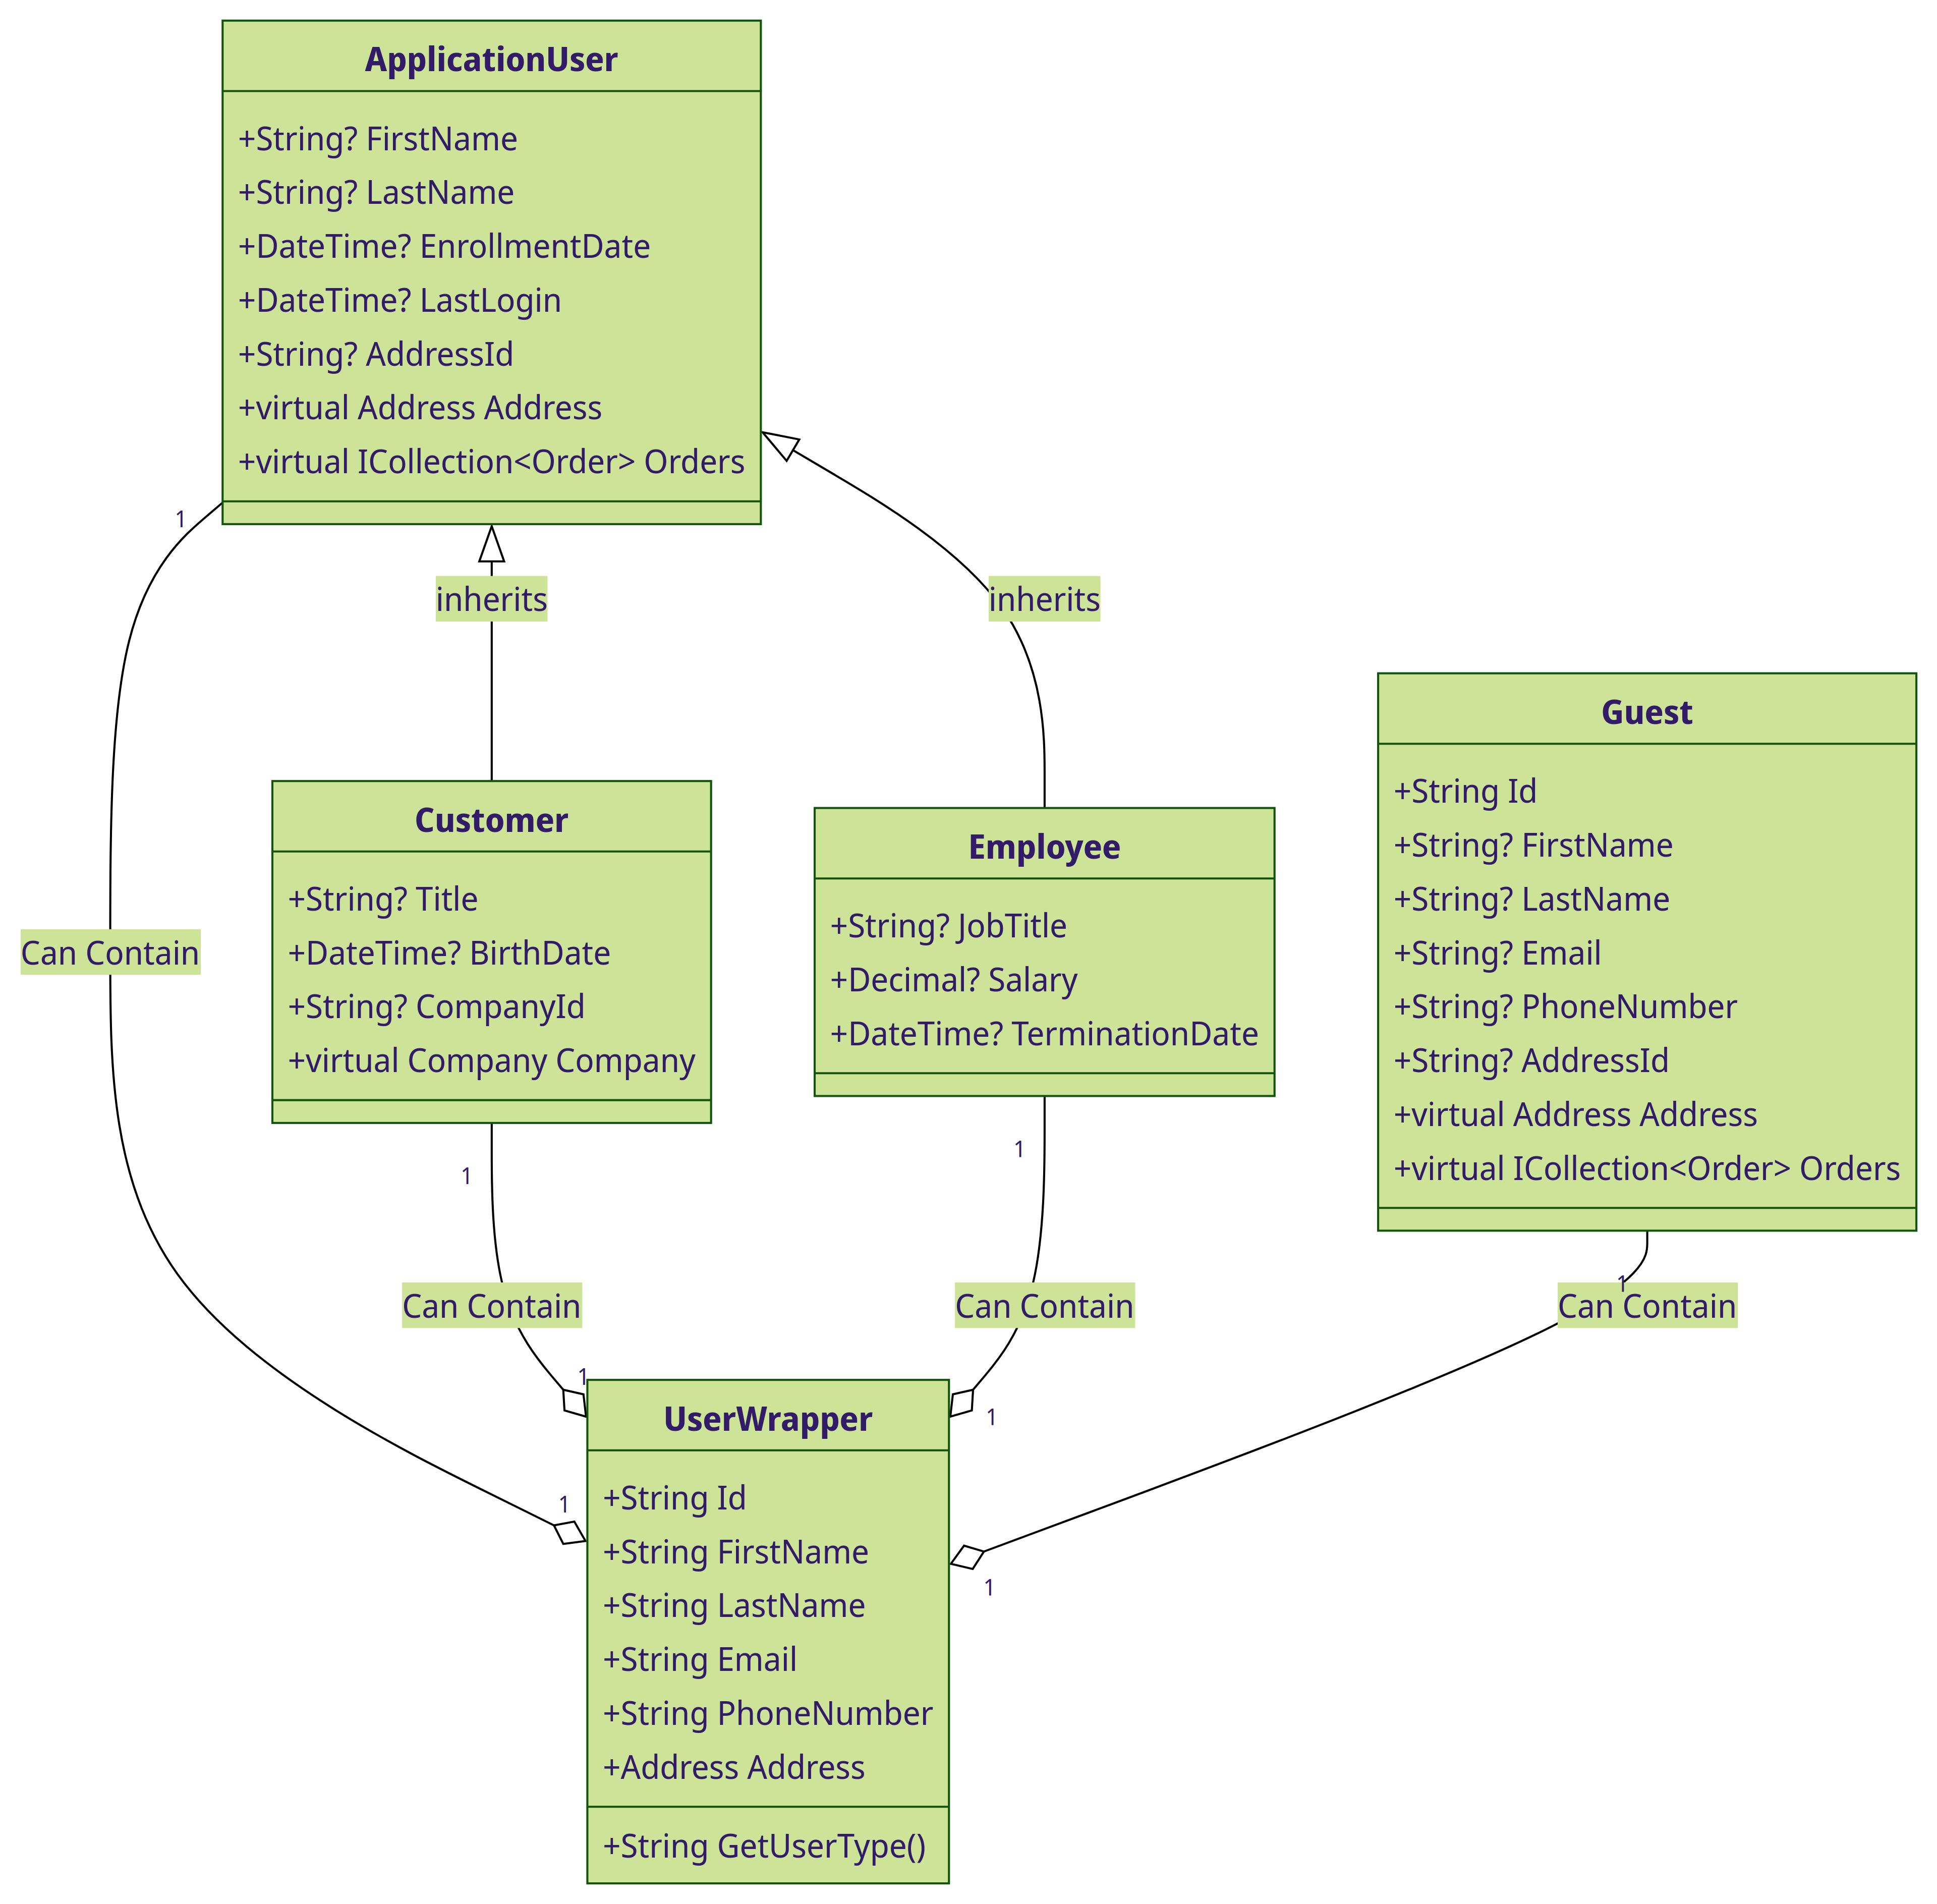
\includegraphics[width=1\textwidth]{figures/diagrams/dcd-user-userwrapper.png}
    \caption{Design Class Diagram - UserWrapper}
    \label{fig:class-diagram-userwrapper}
\end{figure}

\begin{figure}
    \centering
    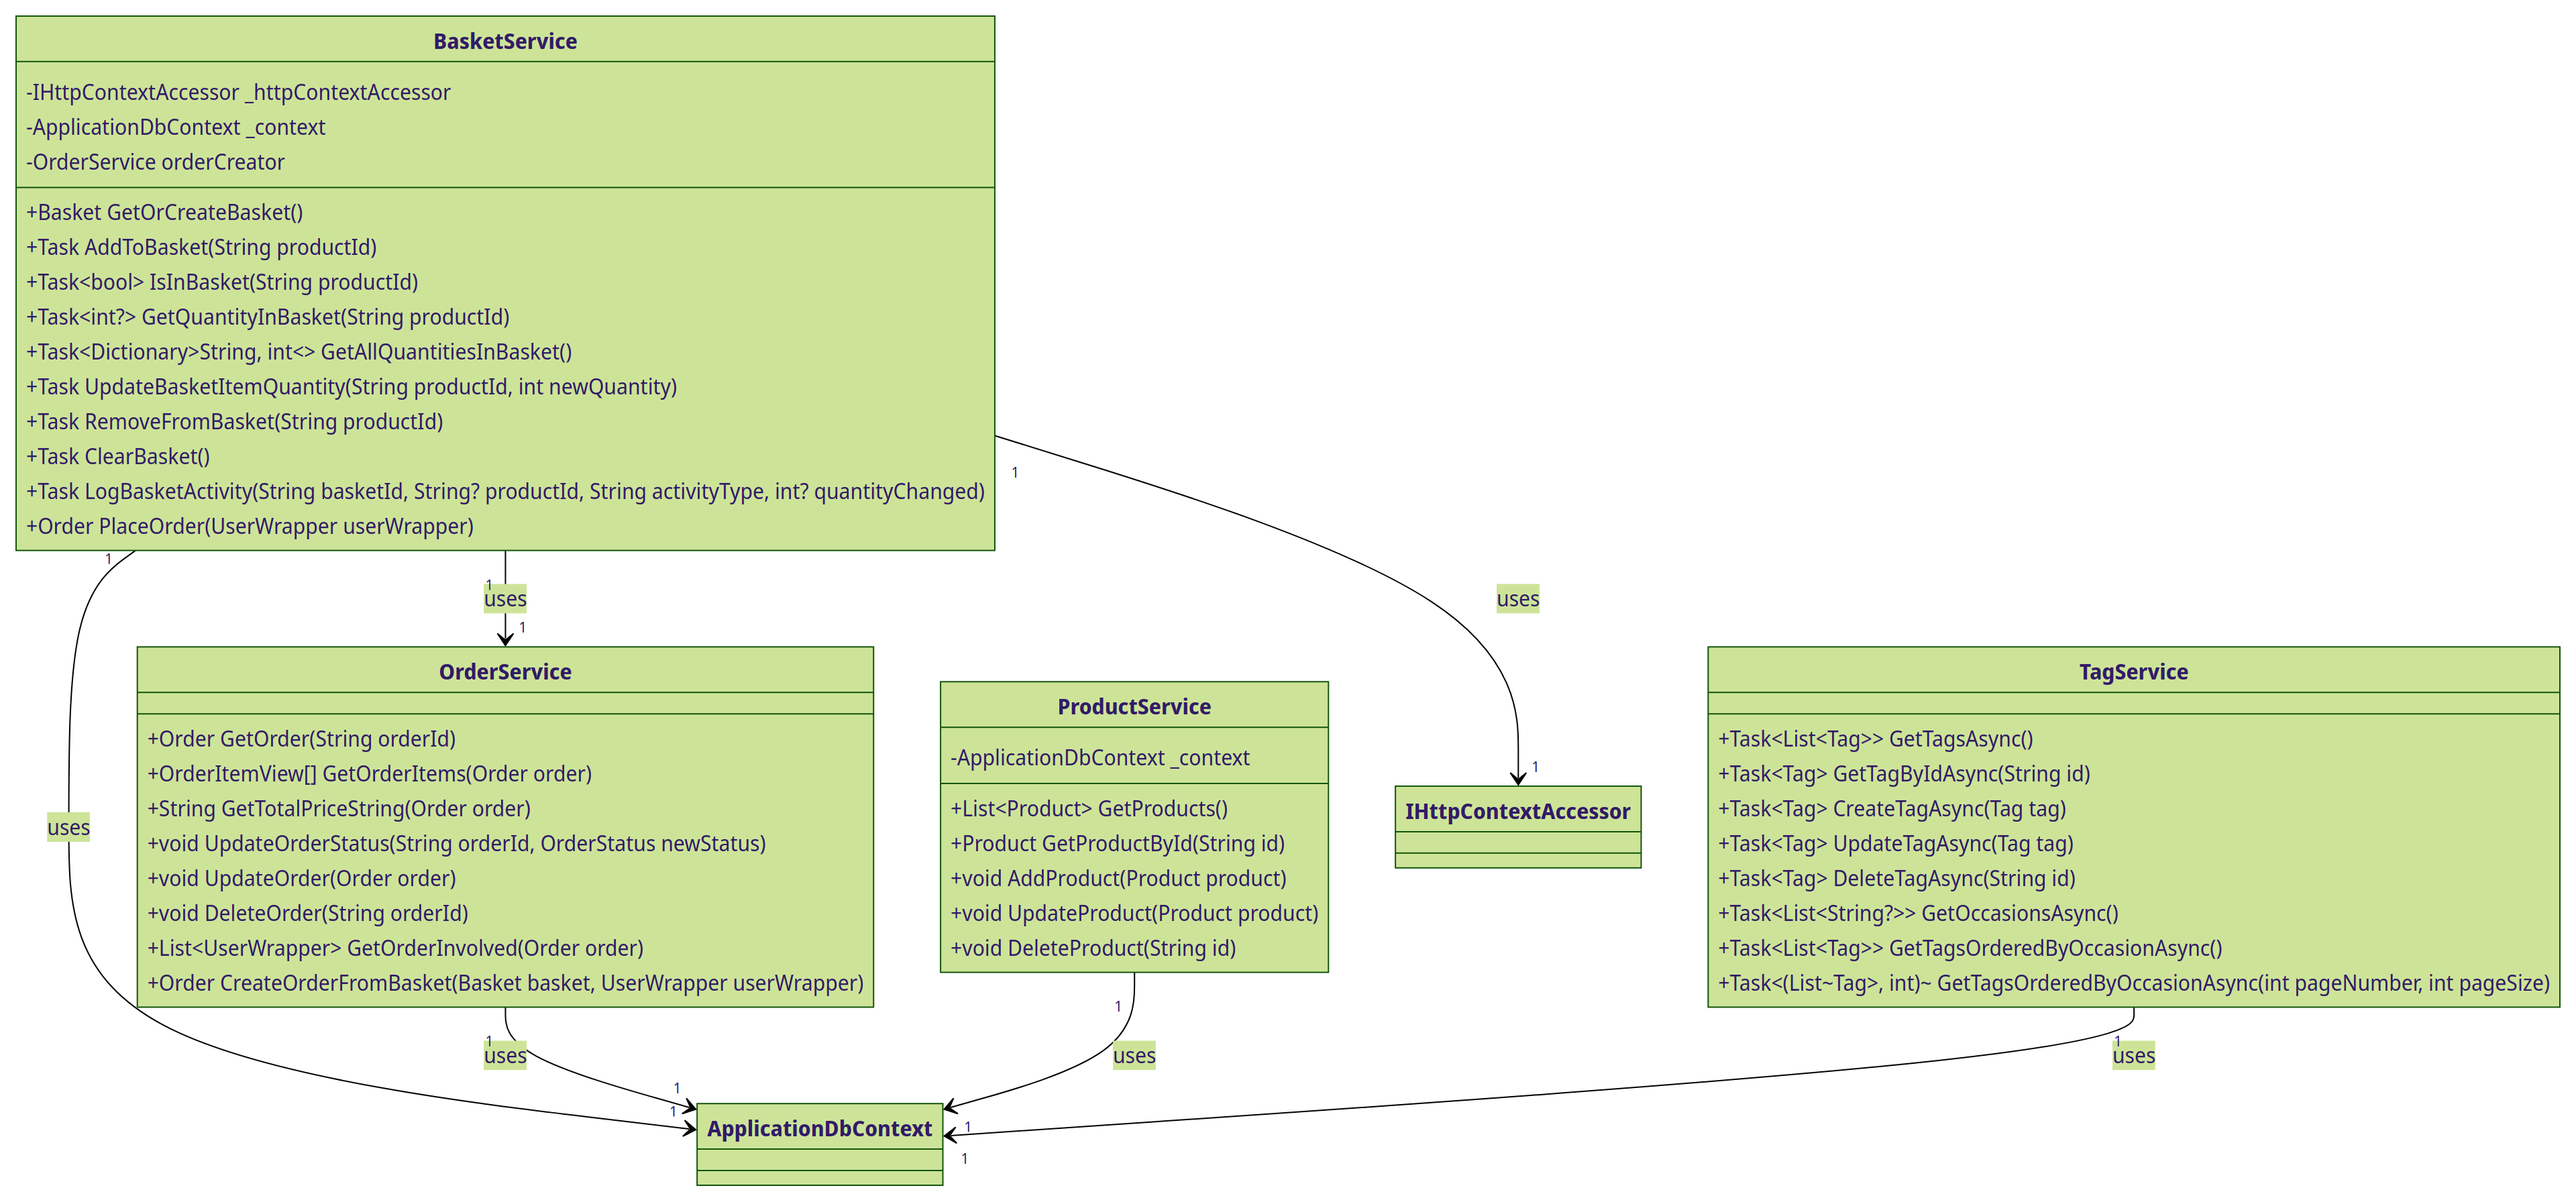
\includegraphics[width=1\textwidth]{figures/diagrams/dcd-main-services.png}
    \caption{Design Class Diagram - Main Services}
    \label{fig:class-diagram-main-services}
\end{figure}

\begin{figure}
    \centering
    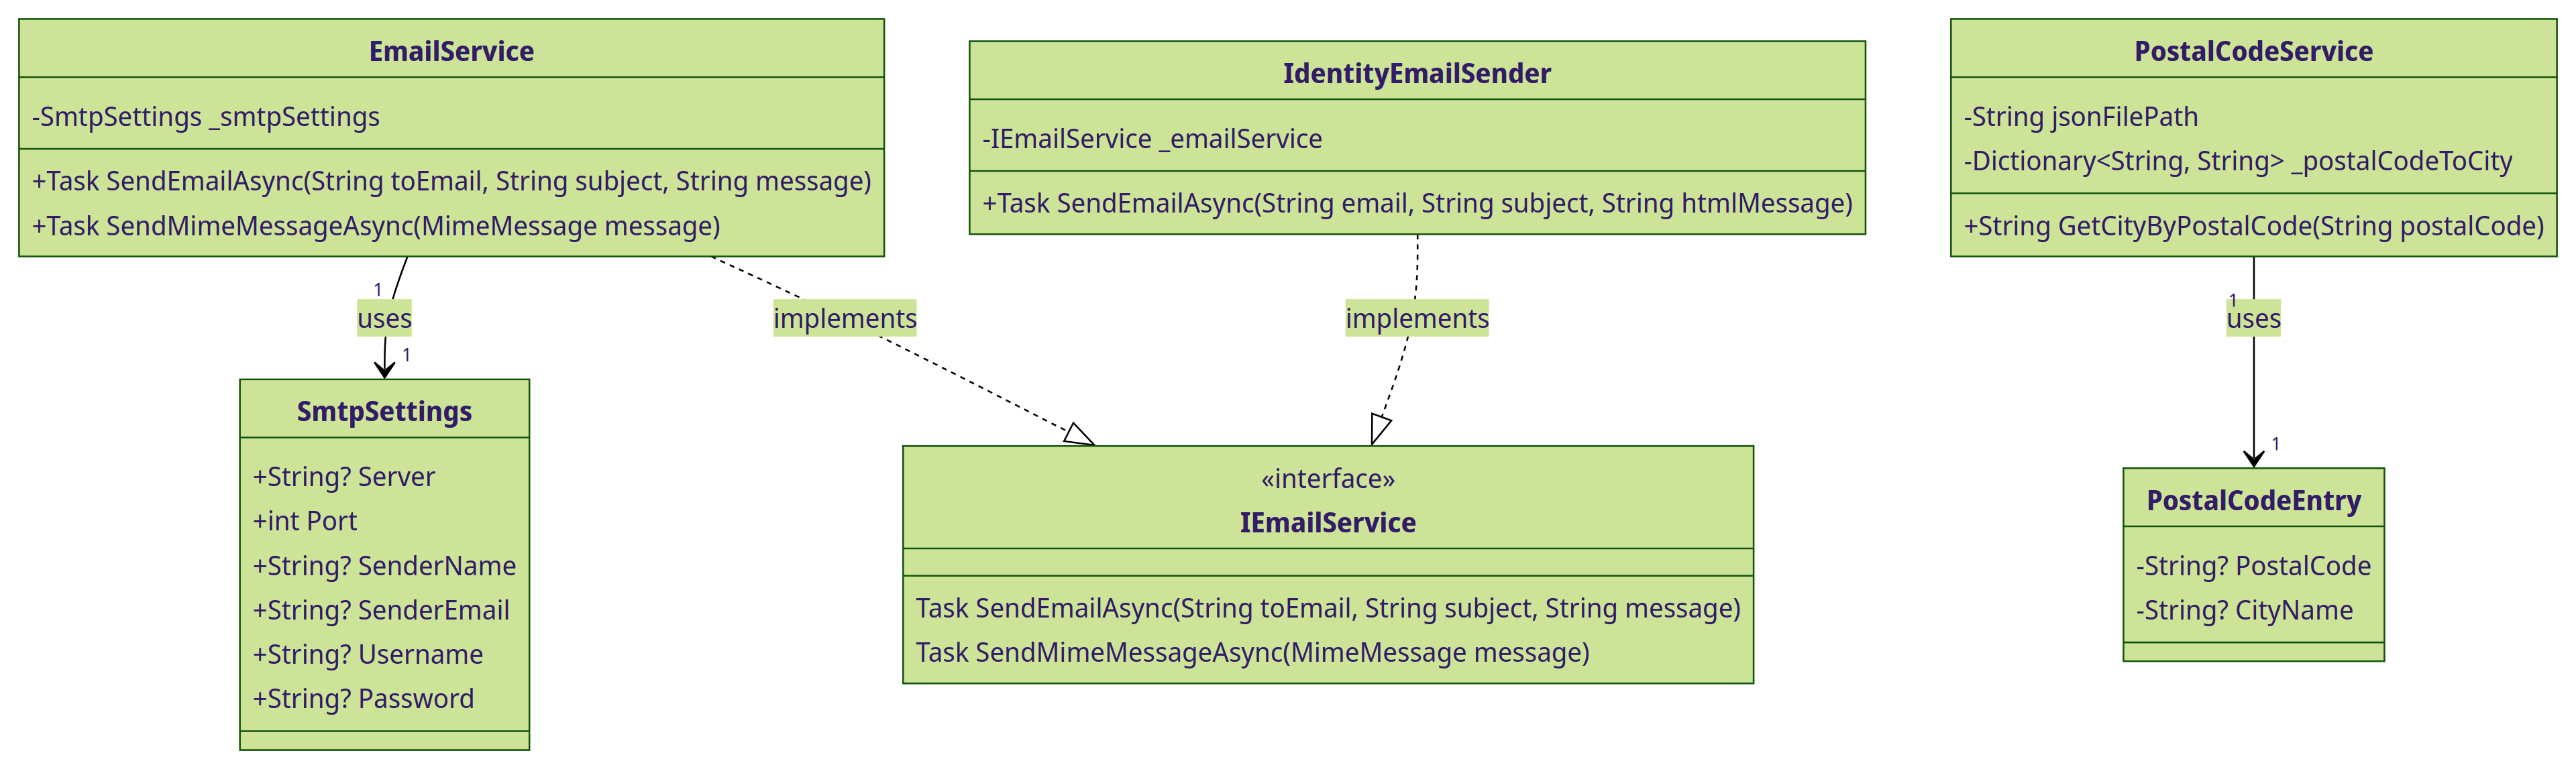
\includegraphics[width=1\textwidth]{figures/diagrams/dcd-aux-services.png}
    \caption{Design Class Diagram - Auxilary Services}
    \label{fig:class-diagram-aux-services}
\end{figure}

\section{Database Diagrammer}

\subsection{Entity Relationship Diagrammer}
\label{appendix:entity-relationship-diagrams}
\begin{figure}
    \centering
    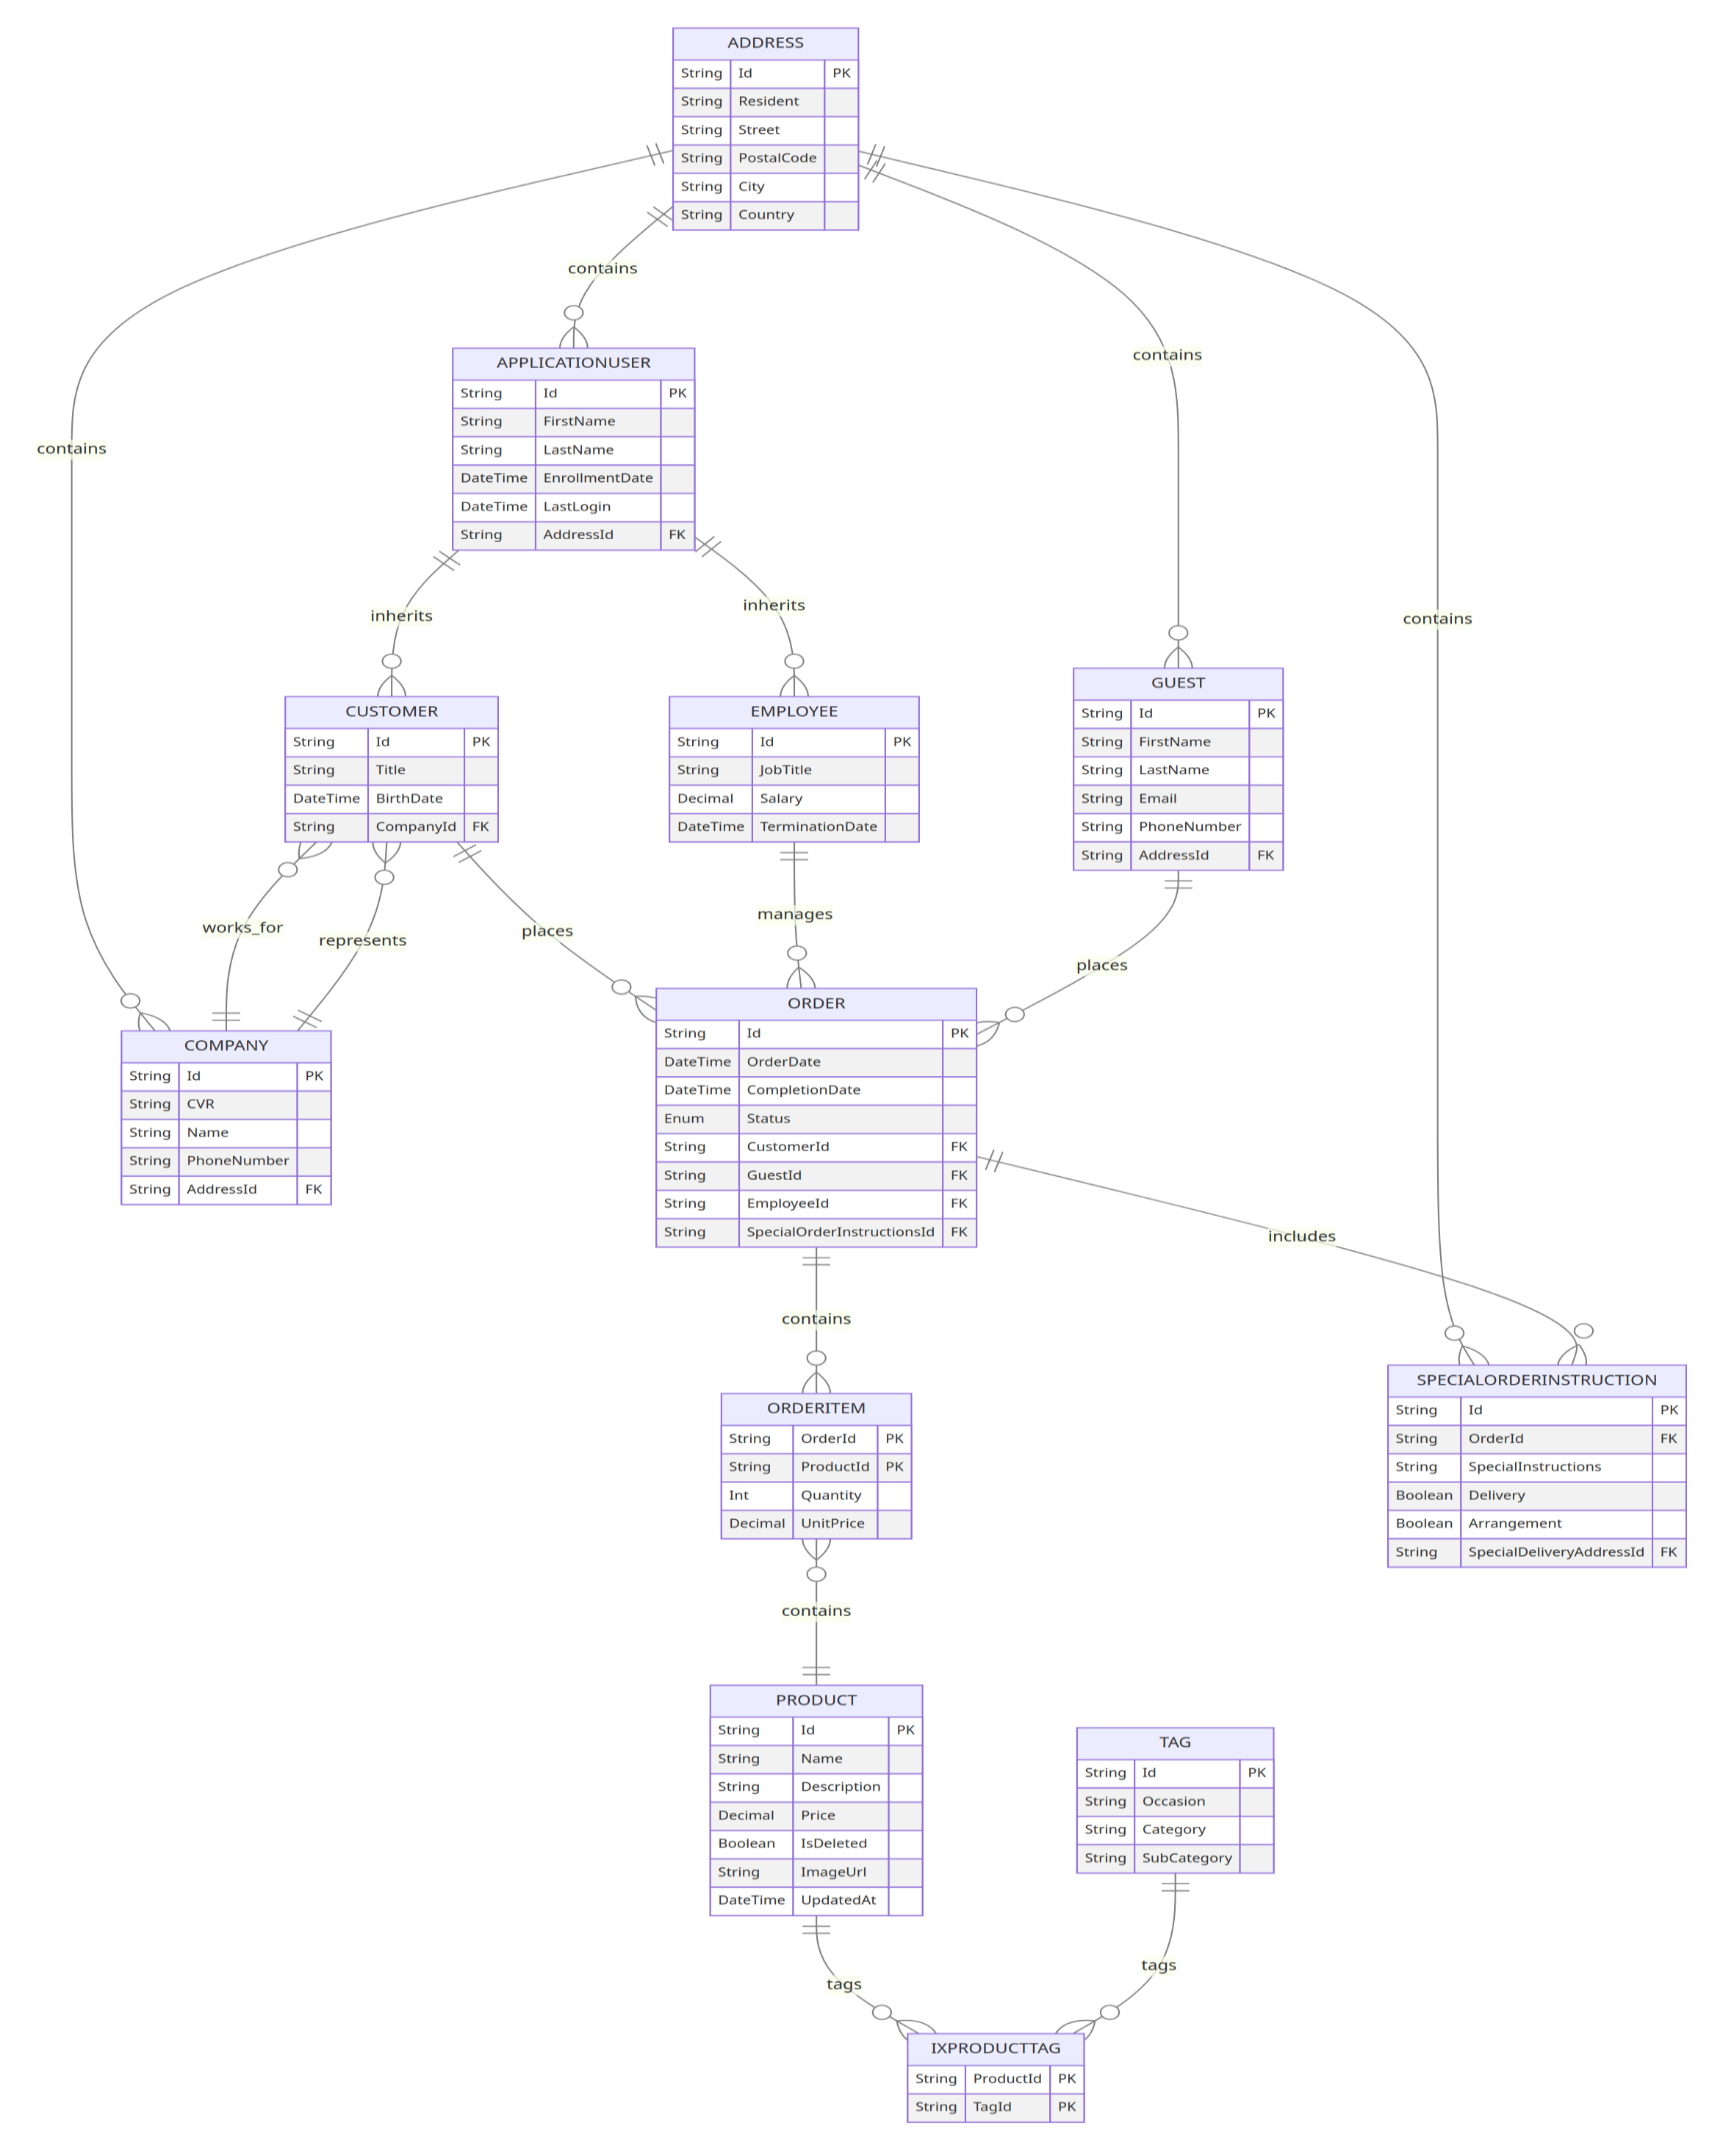
\includegraphics[width=1\textwidth]{figures/diagrams/erd-db-without-basket.png}
    \caption{Entity Relationship Diagram uden basket-relaterede entiteter}
    \label{fig:entity-relationship-diagram-nobasket}
\end{figure}

\begin{figure}
    \centering
    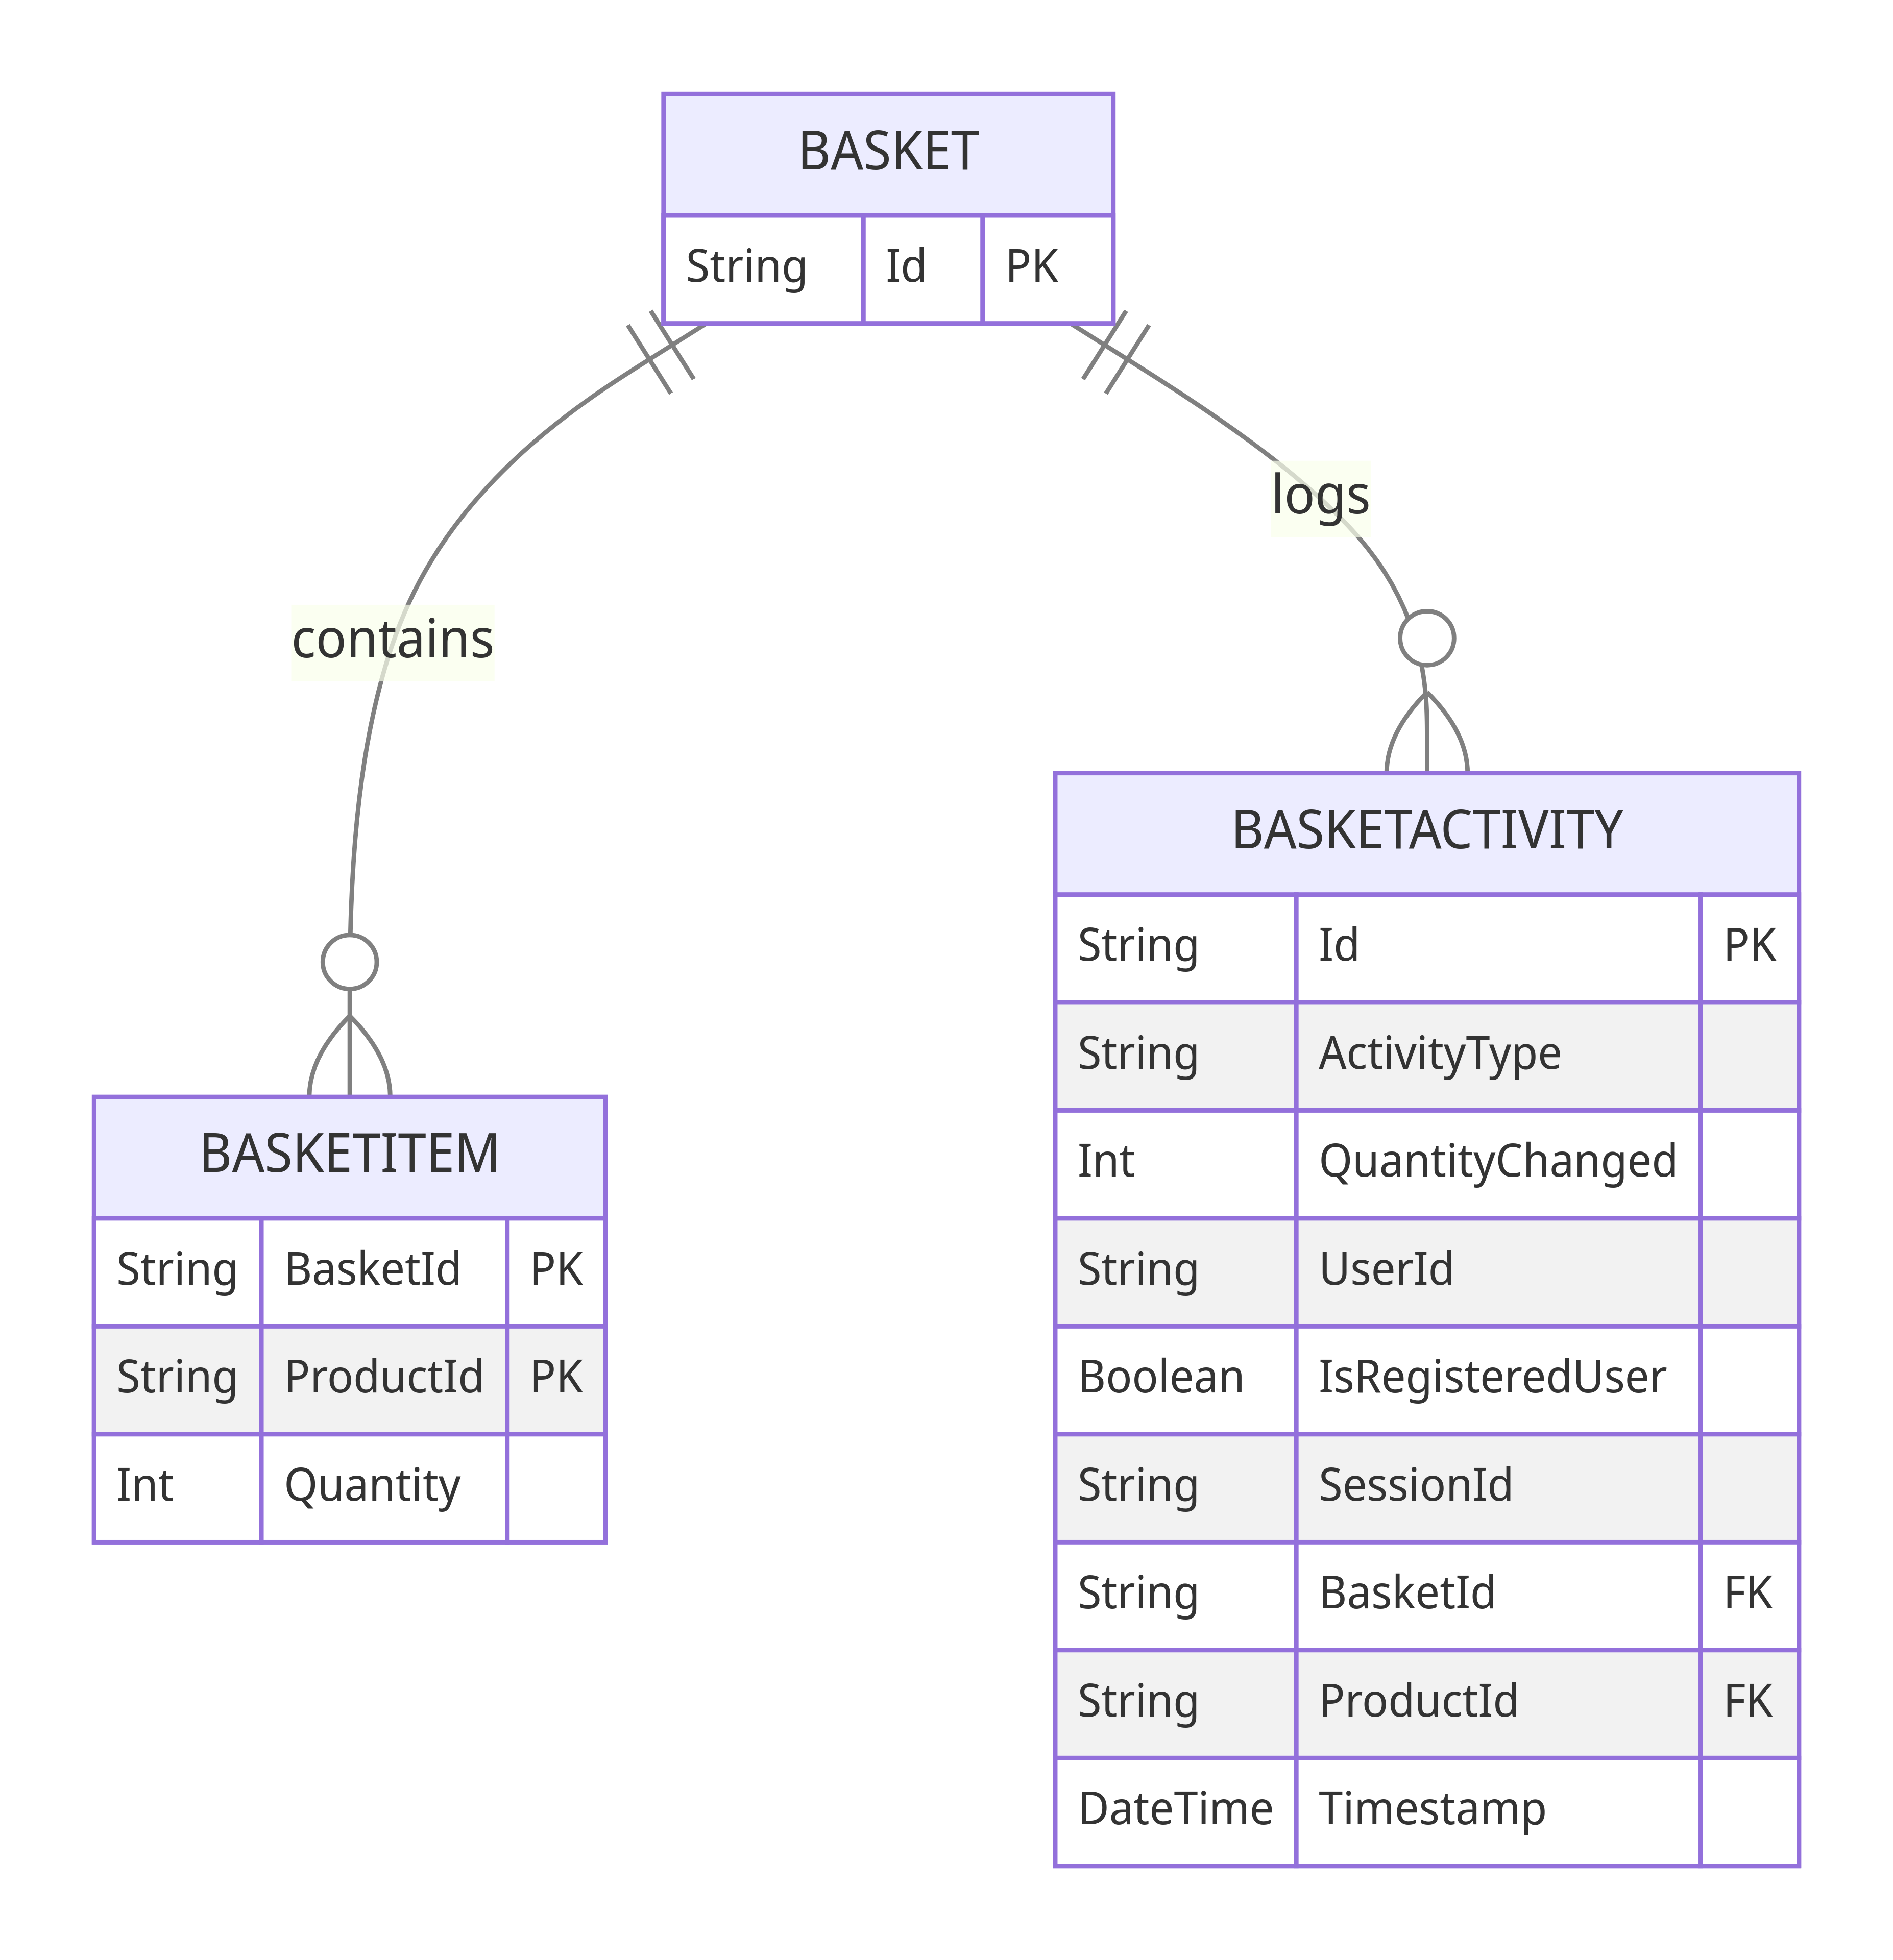
\includegraphics[width=1\textwidth]{figures/diagrams/erd-basket-basketitem-basketact.png}
    \caption{Entity Relationship Diagram kun basket-relaterede entiteter}
    \label{fig:entity-relationship-diagram-basket}
\end{figure}

\subsection{SQL Server Management Studio Diagrammer}
\label{appendix:ssms-diagrams}
\begin{figure}
    \centering
    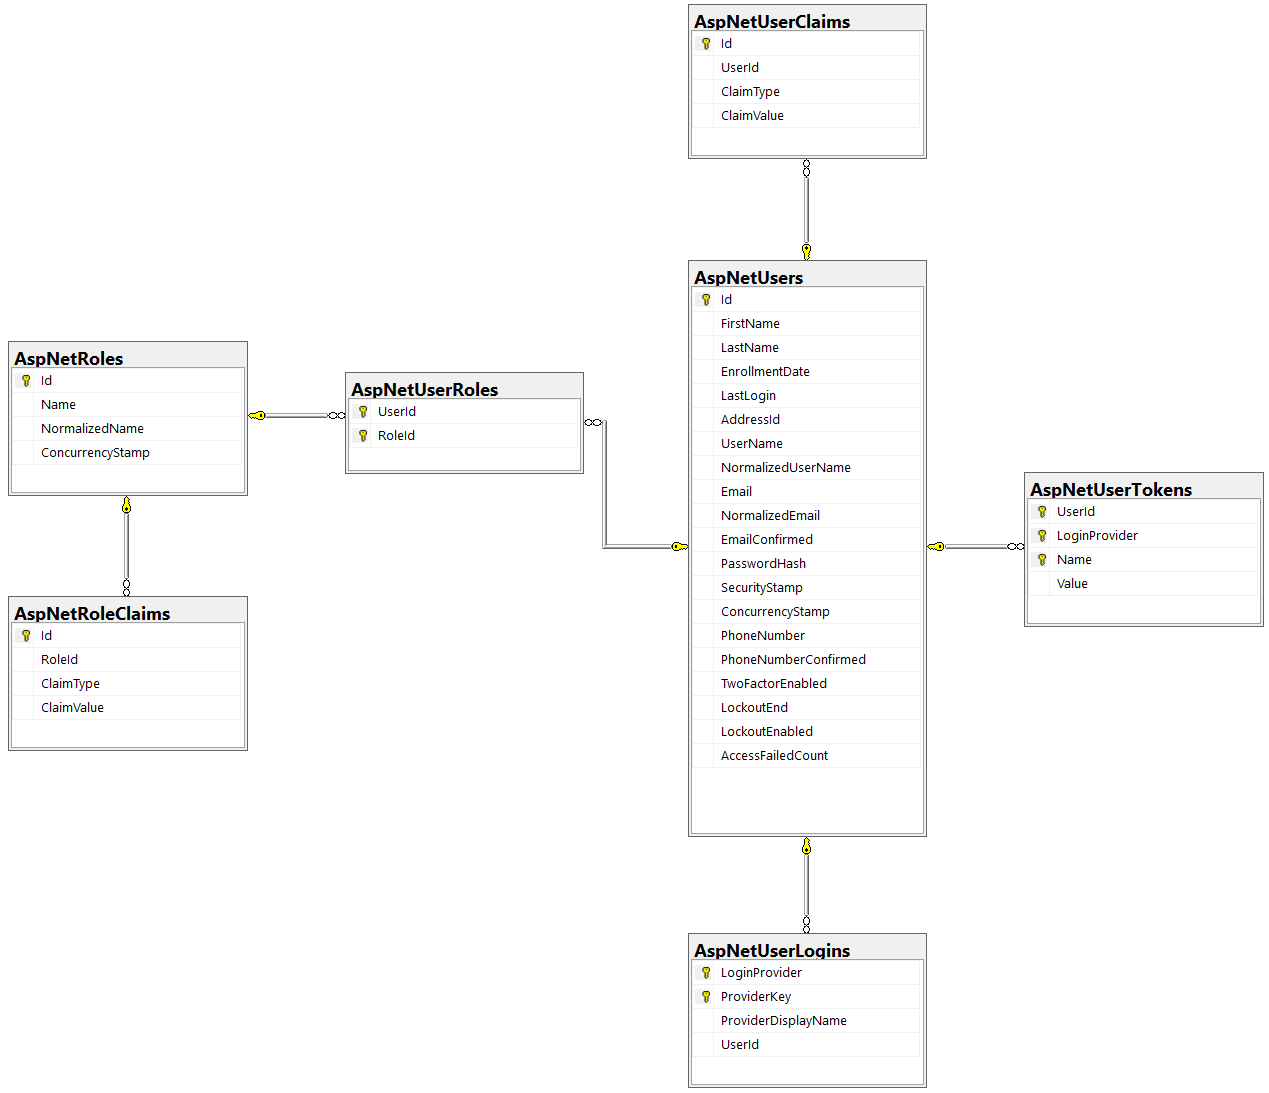
\includegraphics[width=1\textwidth]{figures/ssms/erd-identityusers.png}
    \caption{Database Schema - Users}
    \label{fig:database-schema-users}
\end{figure}

\begin{figure}
    \centering
    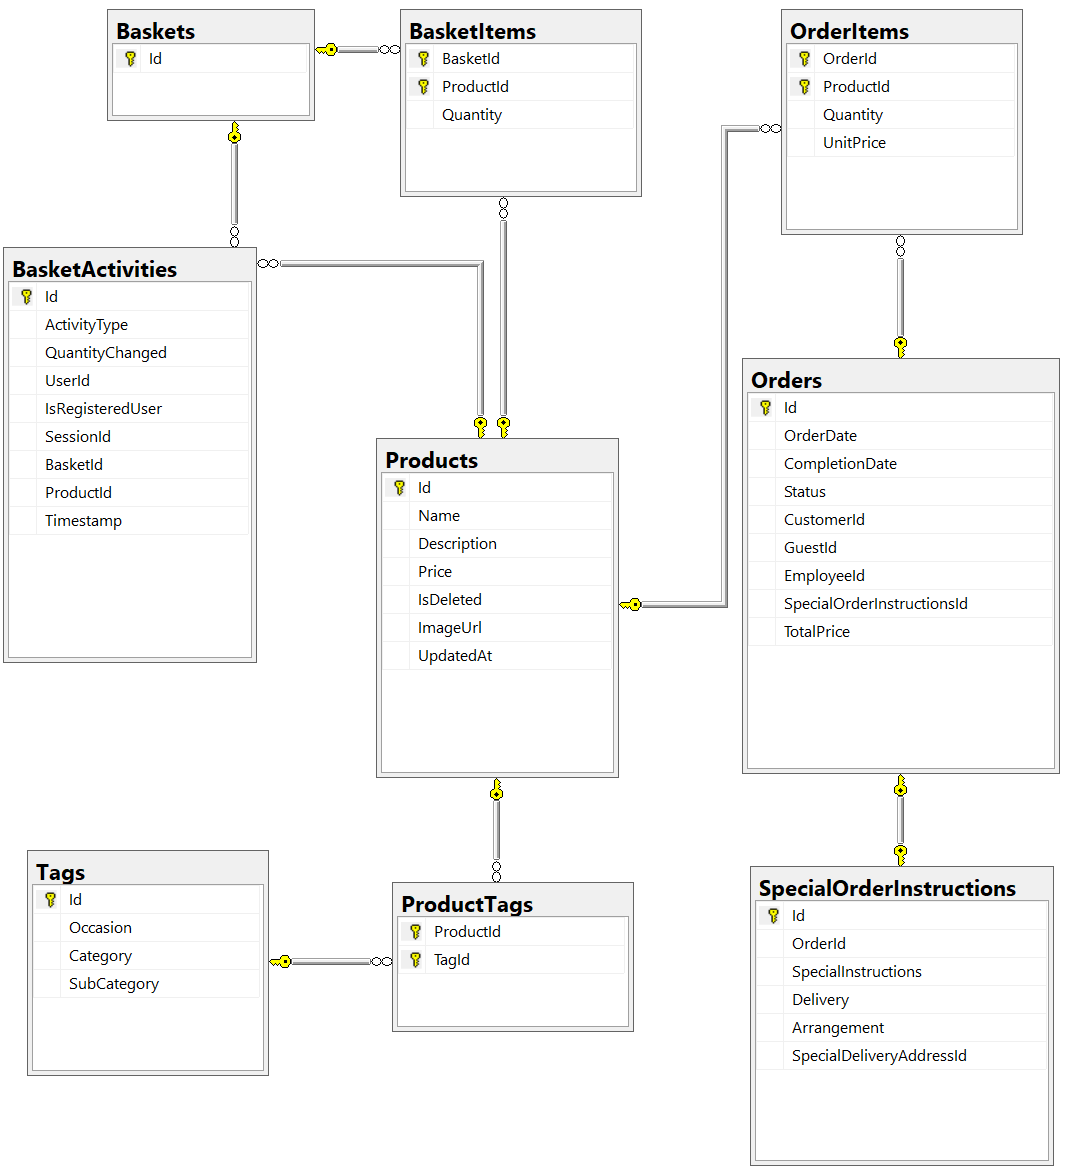
\includegraphics[width=1\textwidth]{figures/ssms/erd-order-products.png}
    \caption{Database Schema - Order Products}
    \label{fig:database-schema-order-products}
\end{figure}

\begin{figure}
    \centering
    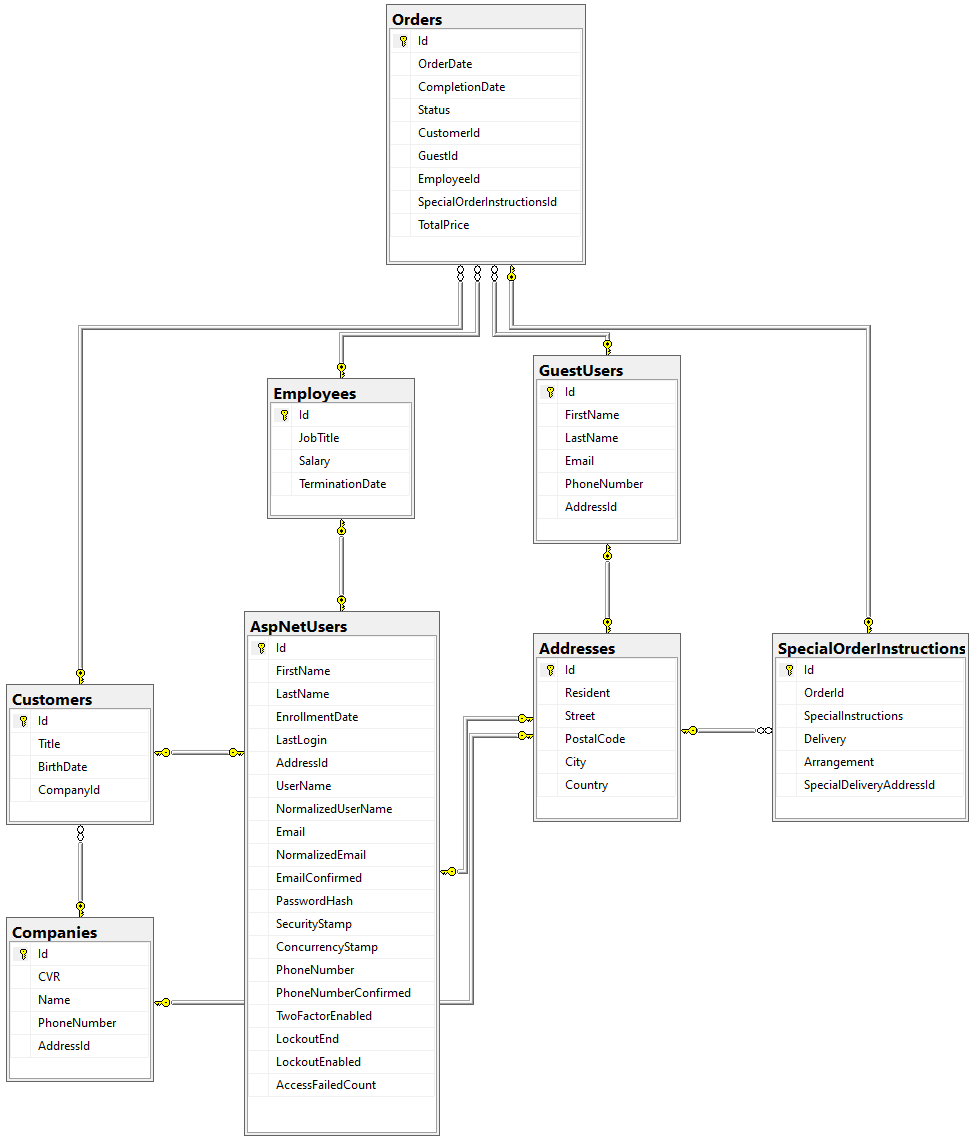
\includegraphics[width=1\textwidth]{figures/ssms/erd-users.png}
    \caption{Database Schema - Basket}
    \label{fig:database-schema-basket}
\end{figure}

\section{Sekvensdiagrammer}
\label{appendix:sequence-diagrams}
\begin{figure}
    \centering
    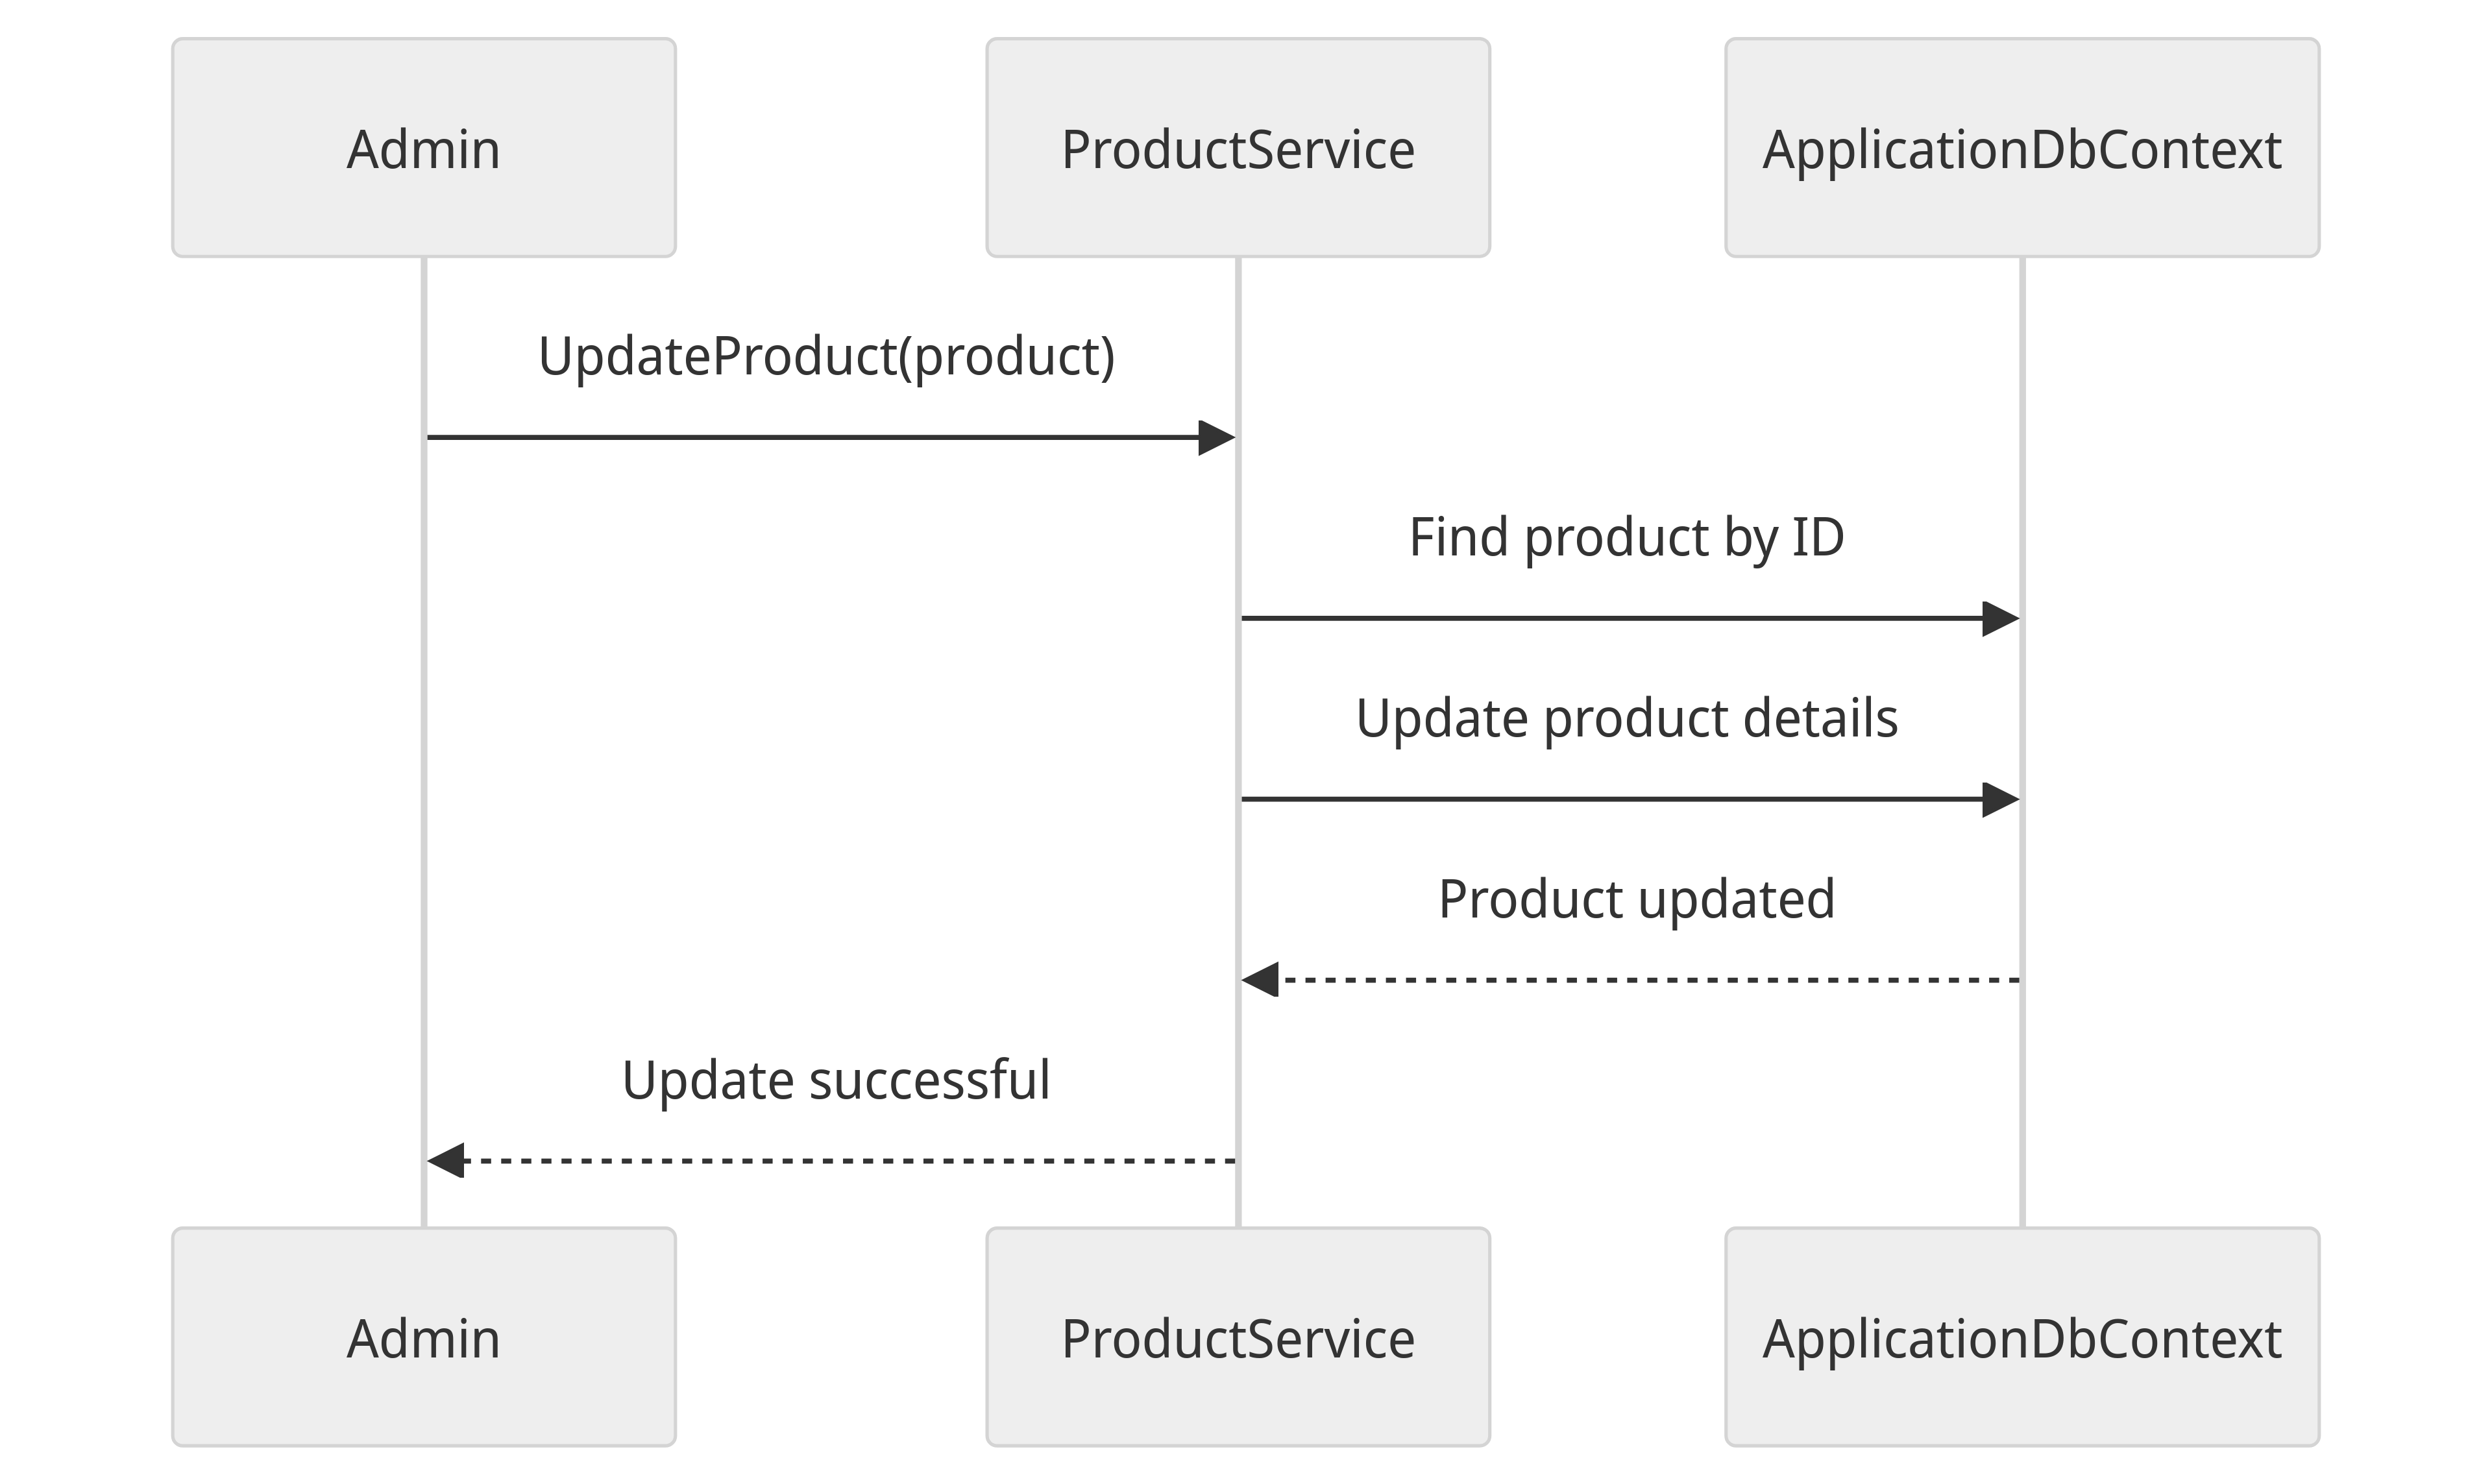
\includegraphics[width=1\textwidth]{figures/diagrams/ssd-admin-updates-product-details.png}
    \caption{System Sequence Diagram - Admin Updates Product Details}
    \label{fig:ssd-admin-updates-product-details}
\end{figure}

\begin{figure}
    \centering
    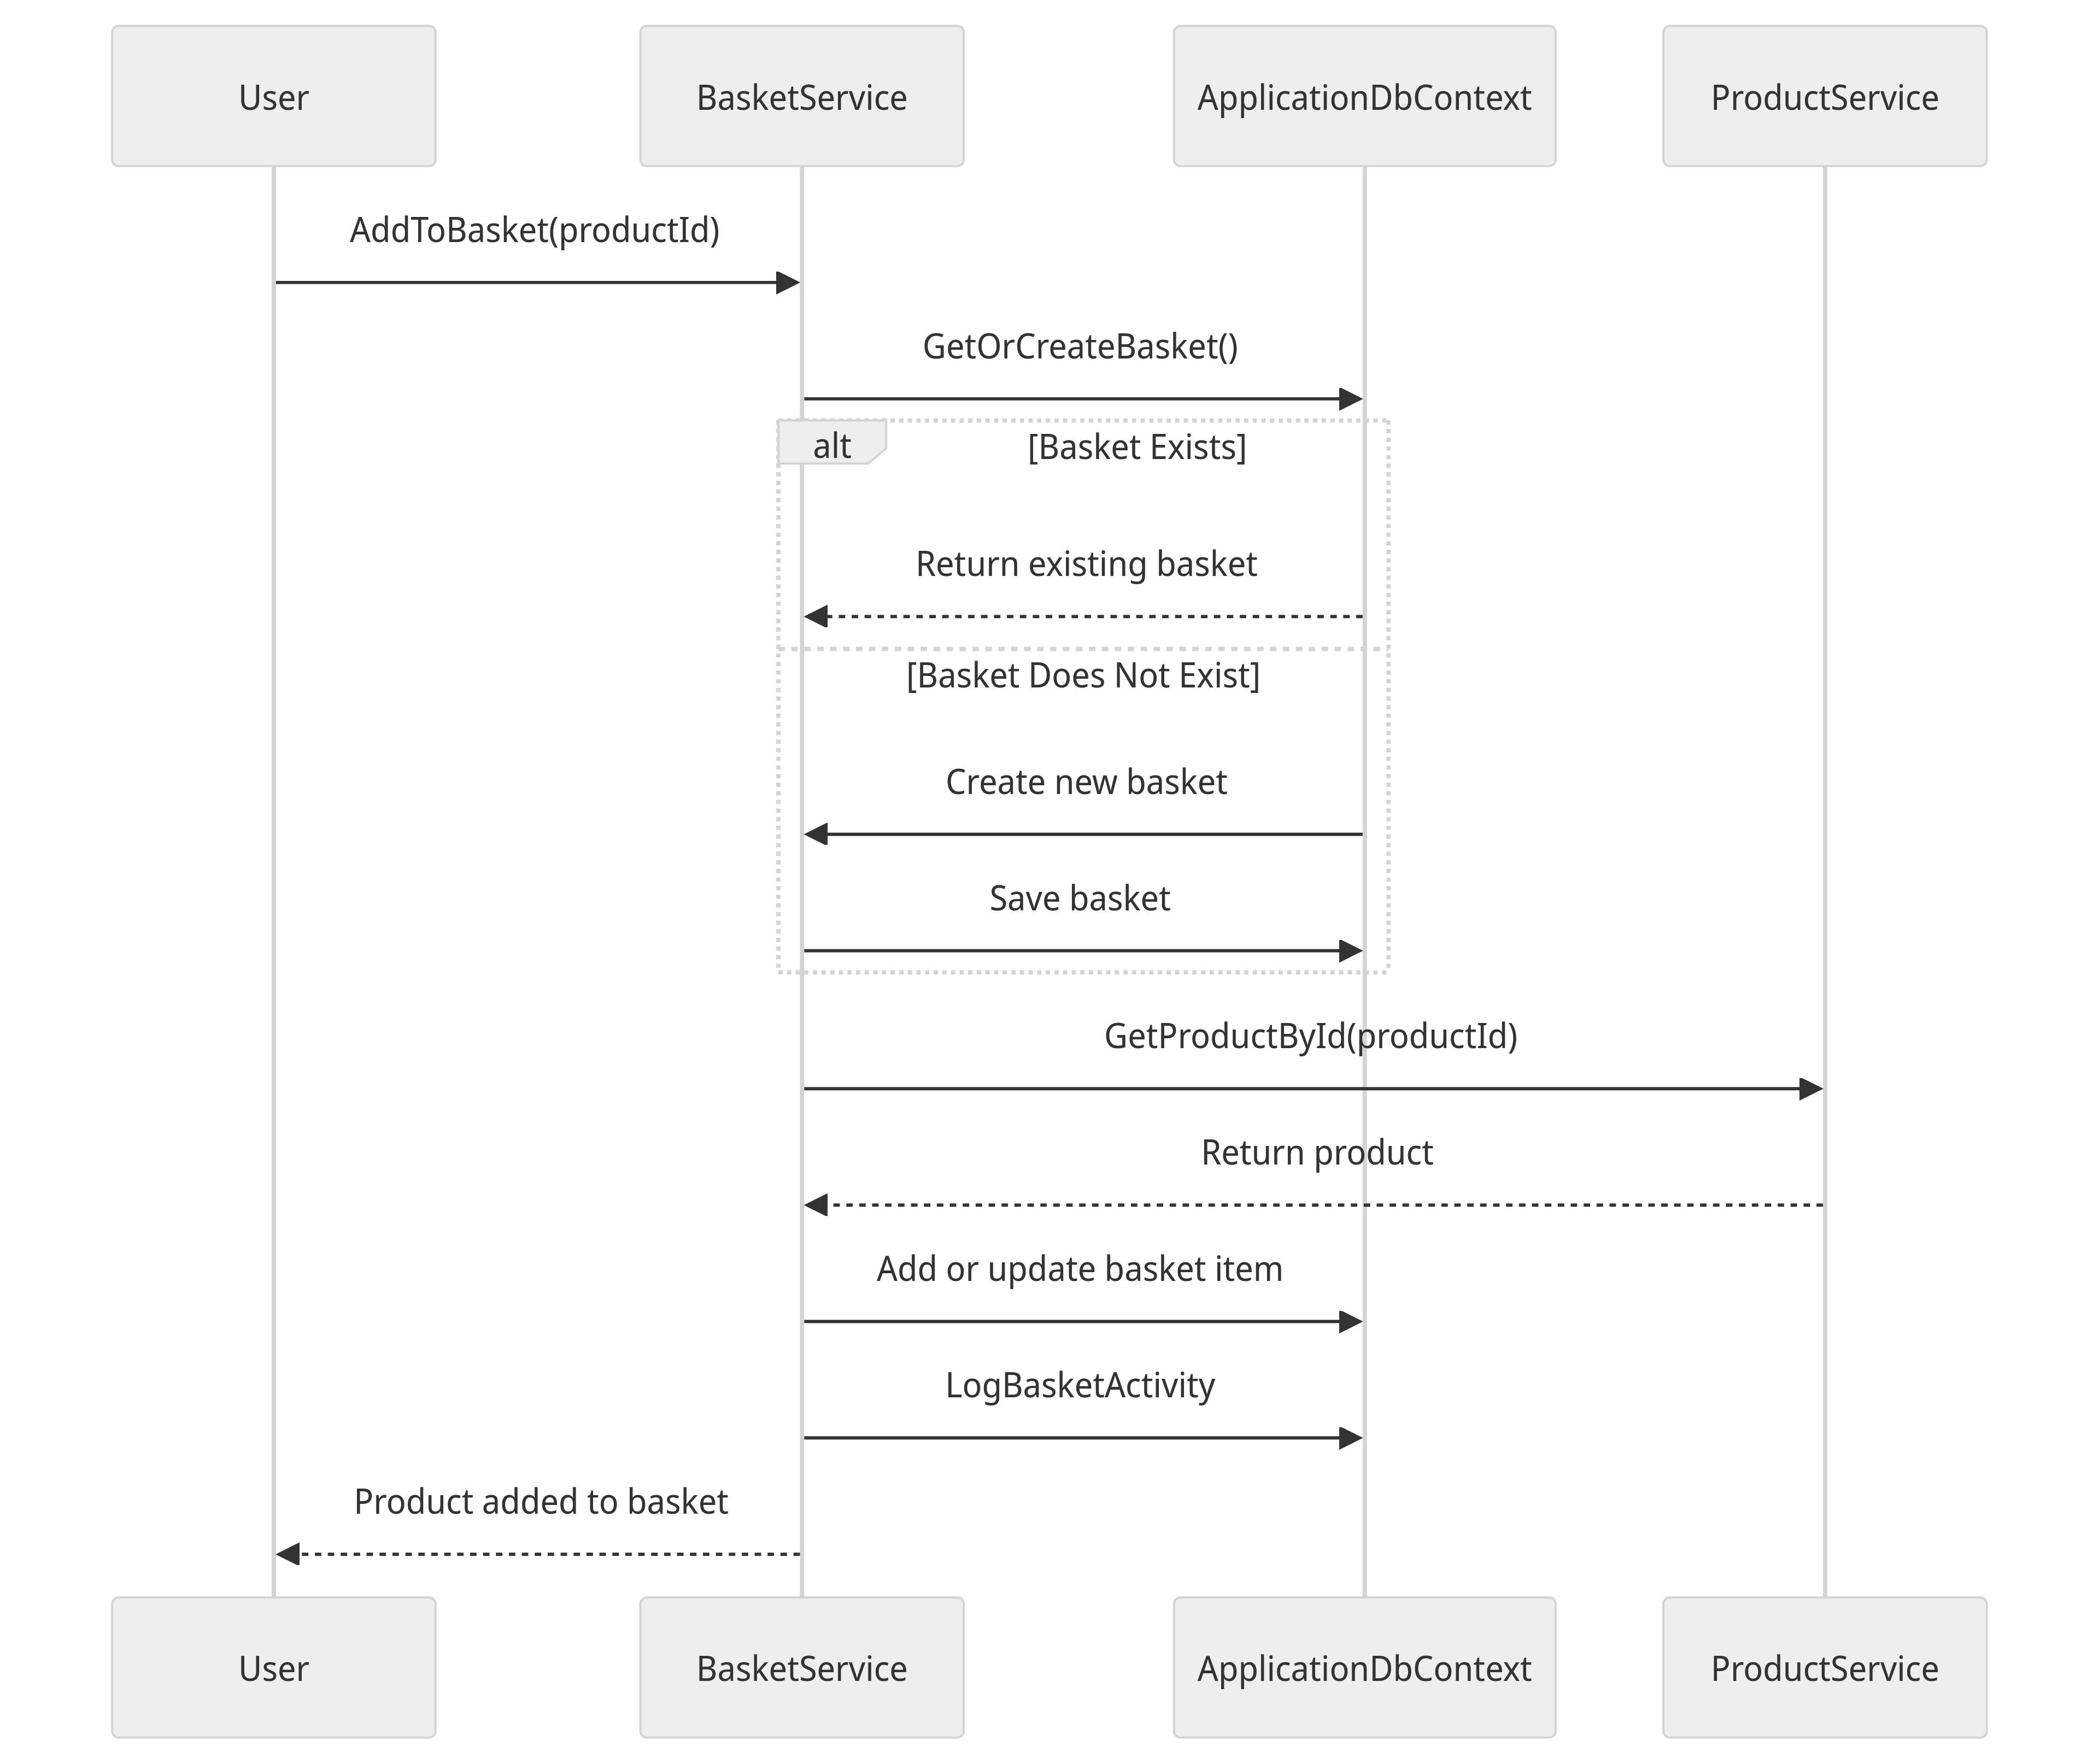
\includegraphics[width=1\textwidth]{figures/diagrams/ssd-user-adds-product-to-basket.png}
    \caption{System Sequence Diagram - User Adds Product to Basket}
    \label{fig:ssd-user-adds-product-to-basket}
\end{figure}

\begin{figure}
    \centering
    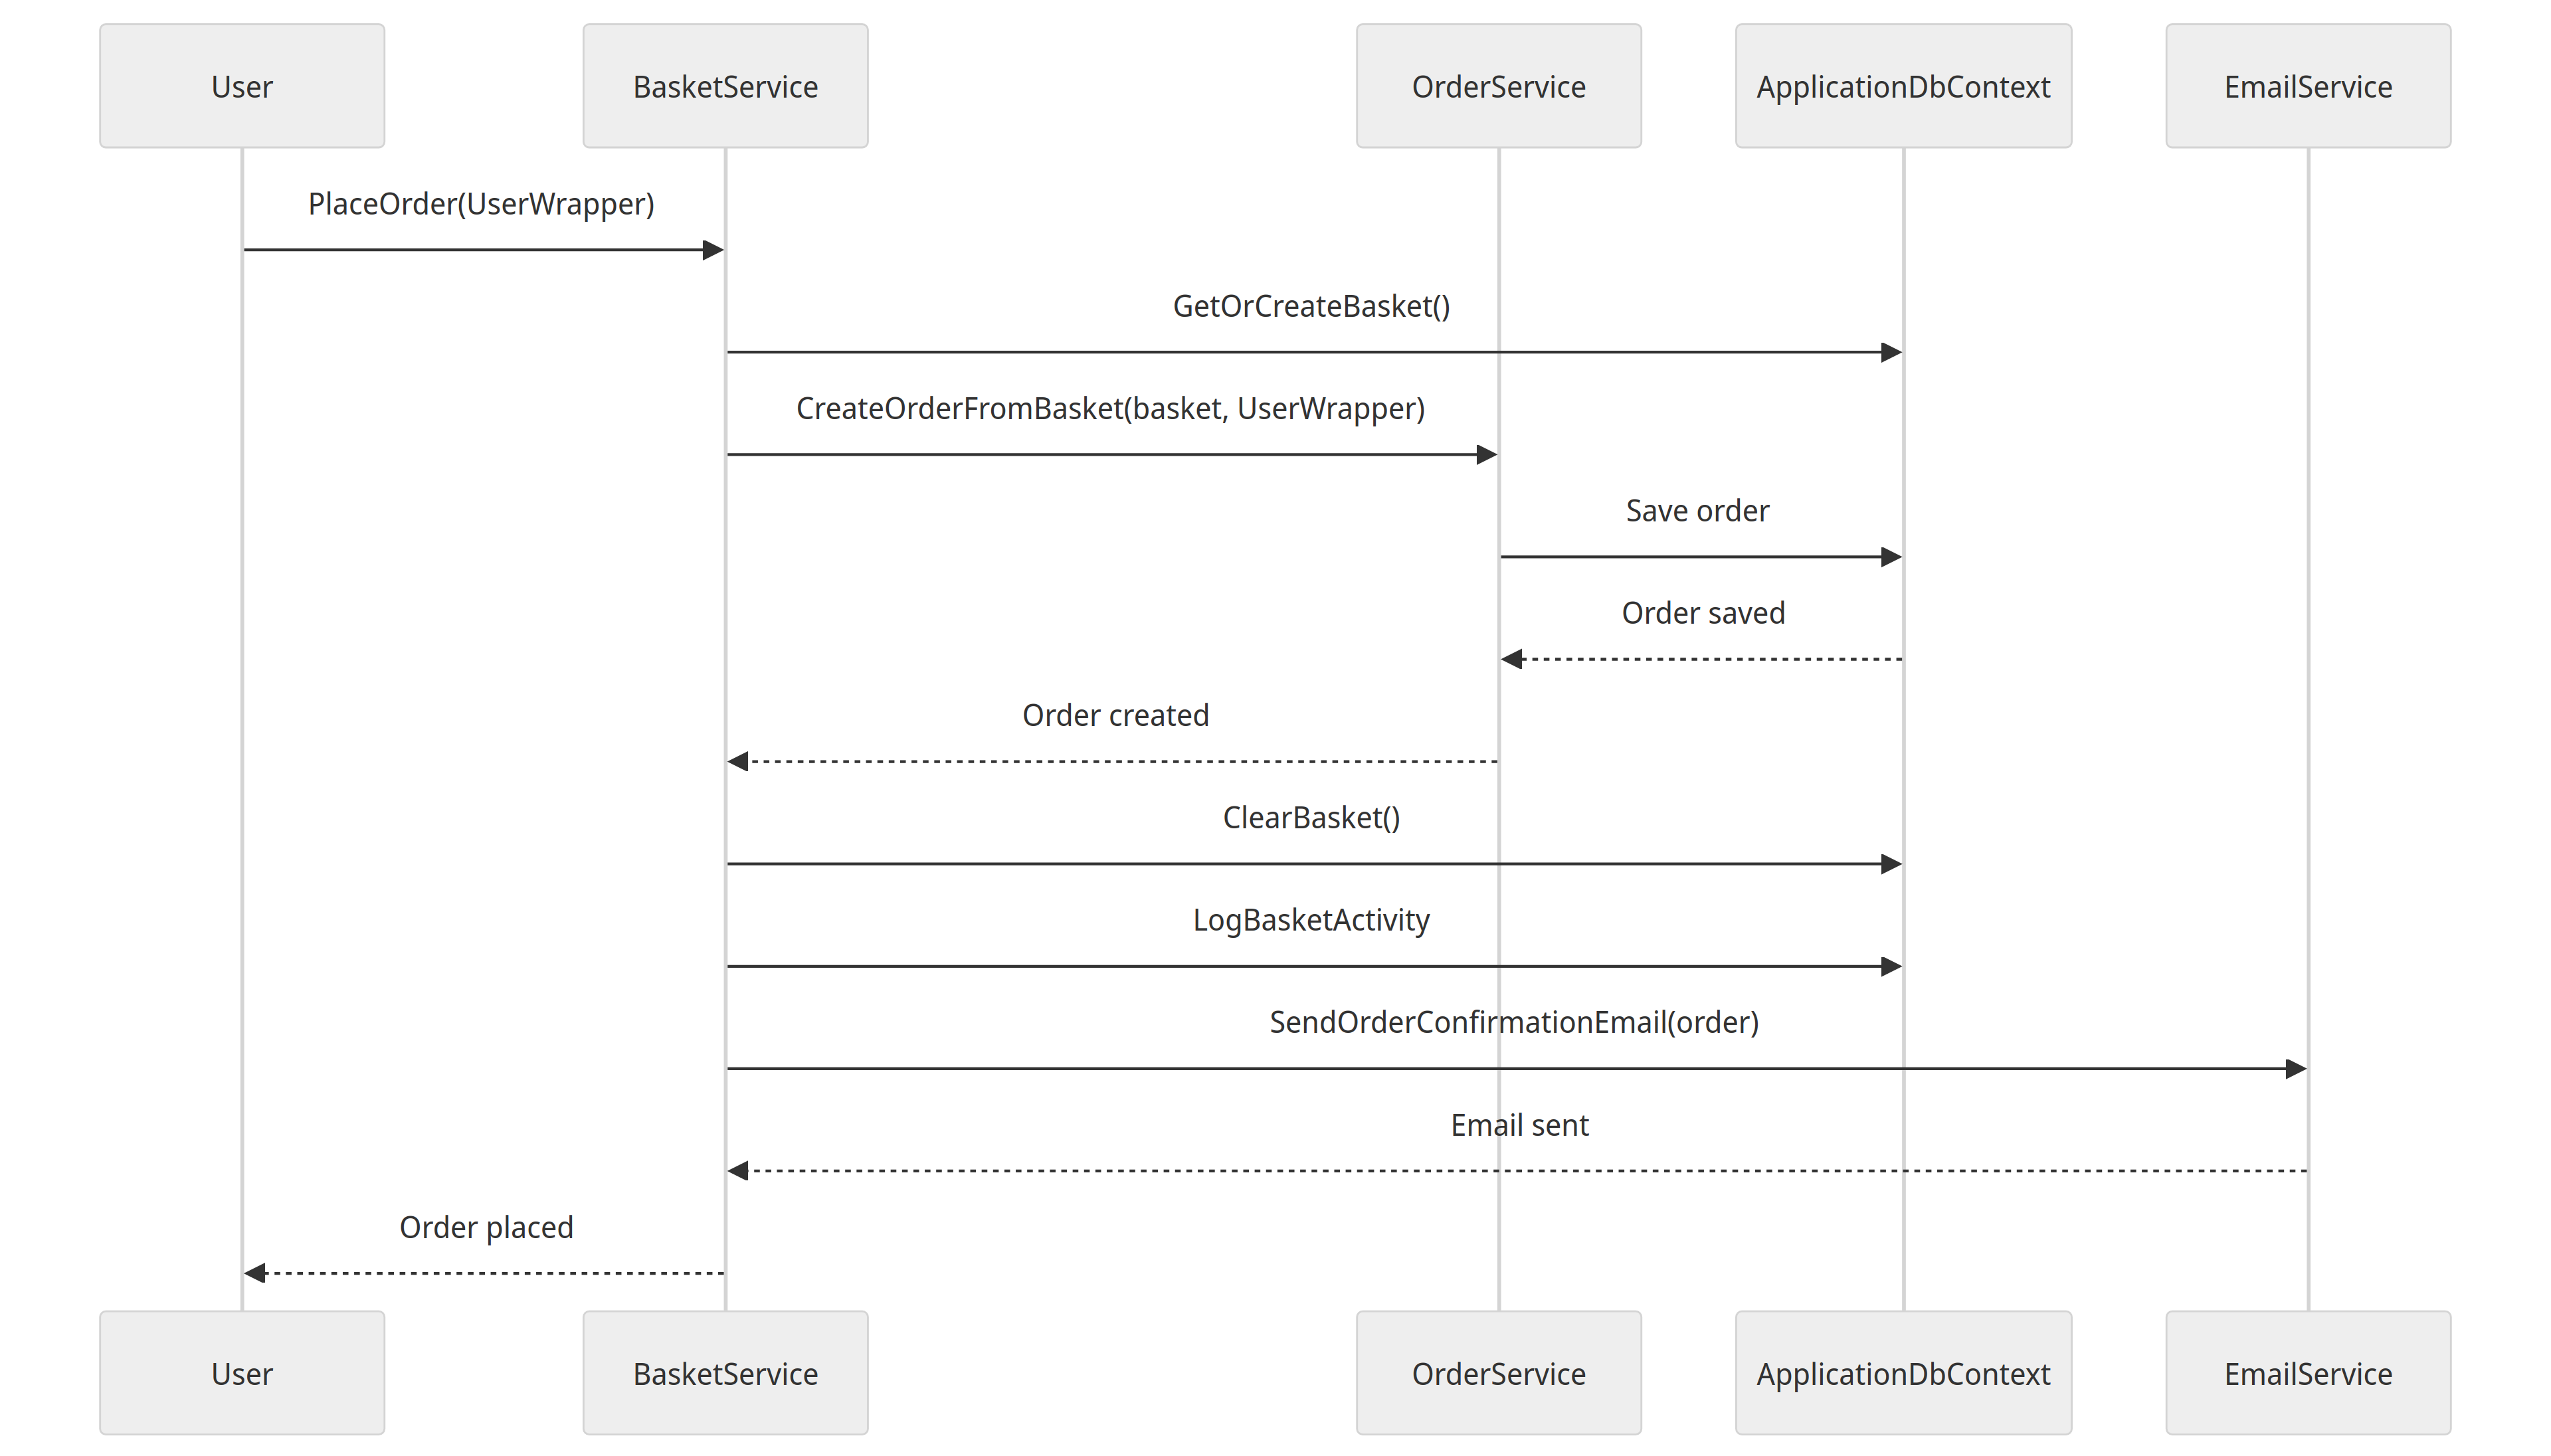
\includegraphics[width=1\textwidth]{figures/diagrams/ssd-user-places-an-order.png}
    \caption{System Sequence Diagram - User Places Order}
    \label{fig:ssd-user-places-order}
\end{figure}

\begin{figure}
    \centering
    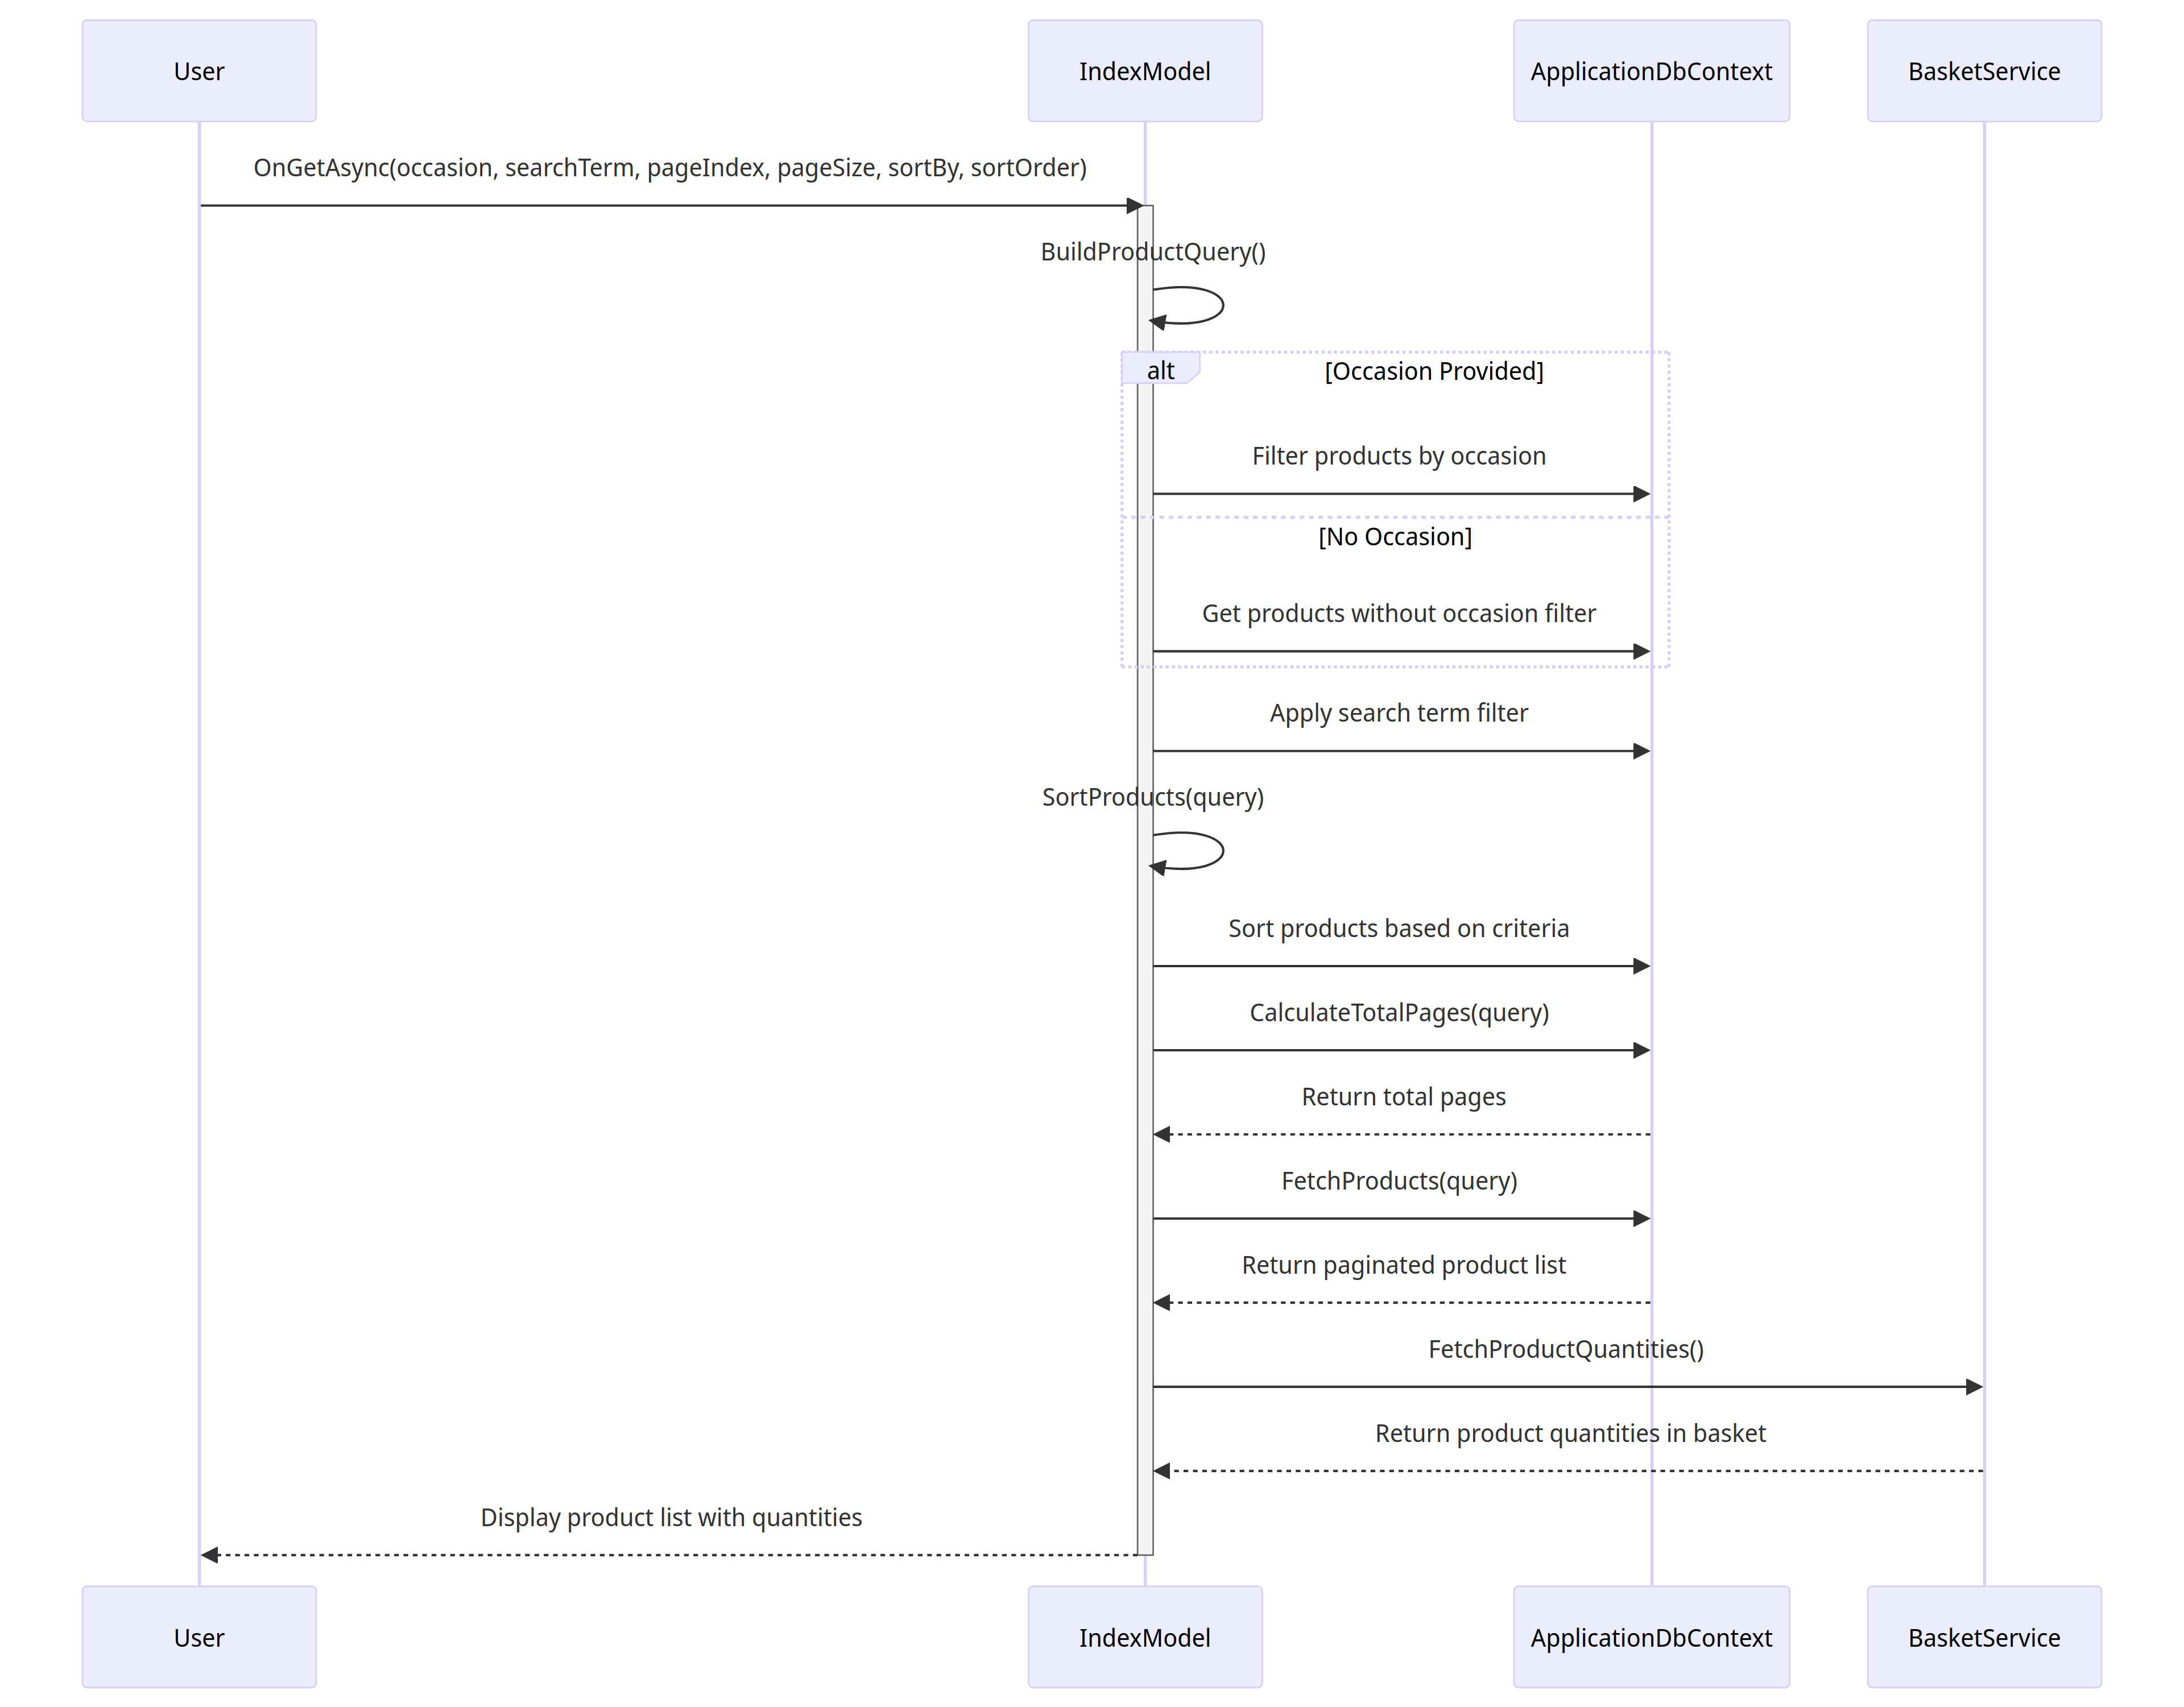
\includegraphics[width=1\textwidth]{figures/diagrams/ssd-ongetasync-customerproducts-index.png}
    \caption{System Sequence Diagram - OnGetAsync CustomerProducts Index}
    \label{fig:ssd-ongetasync-customerproducts-index}
\end{figure}

\begin{figure}
    \centering
    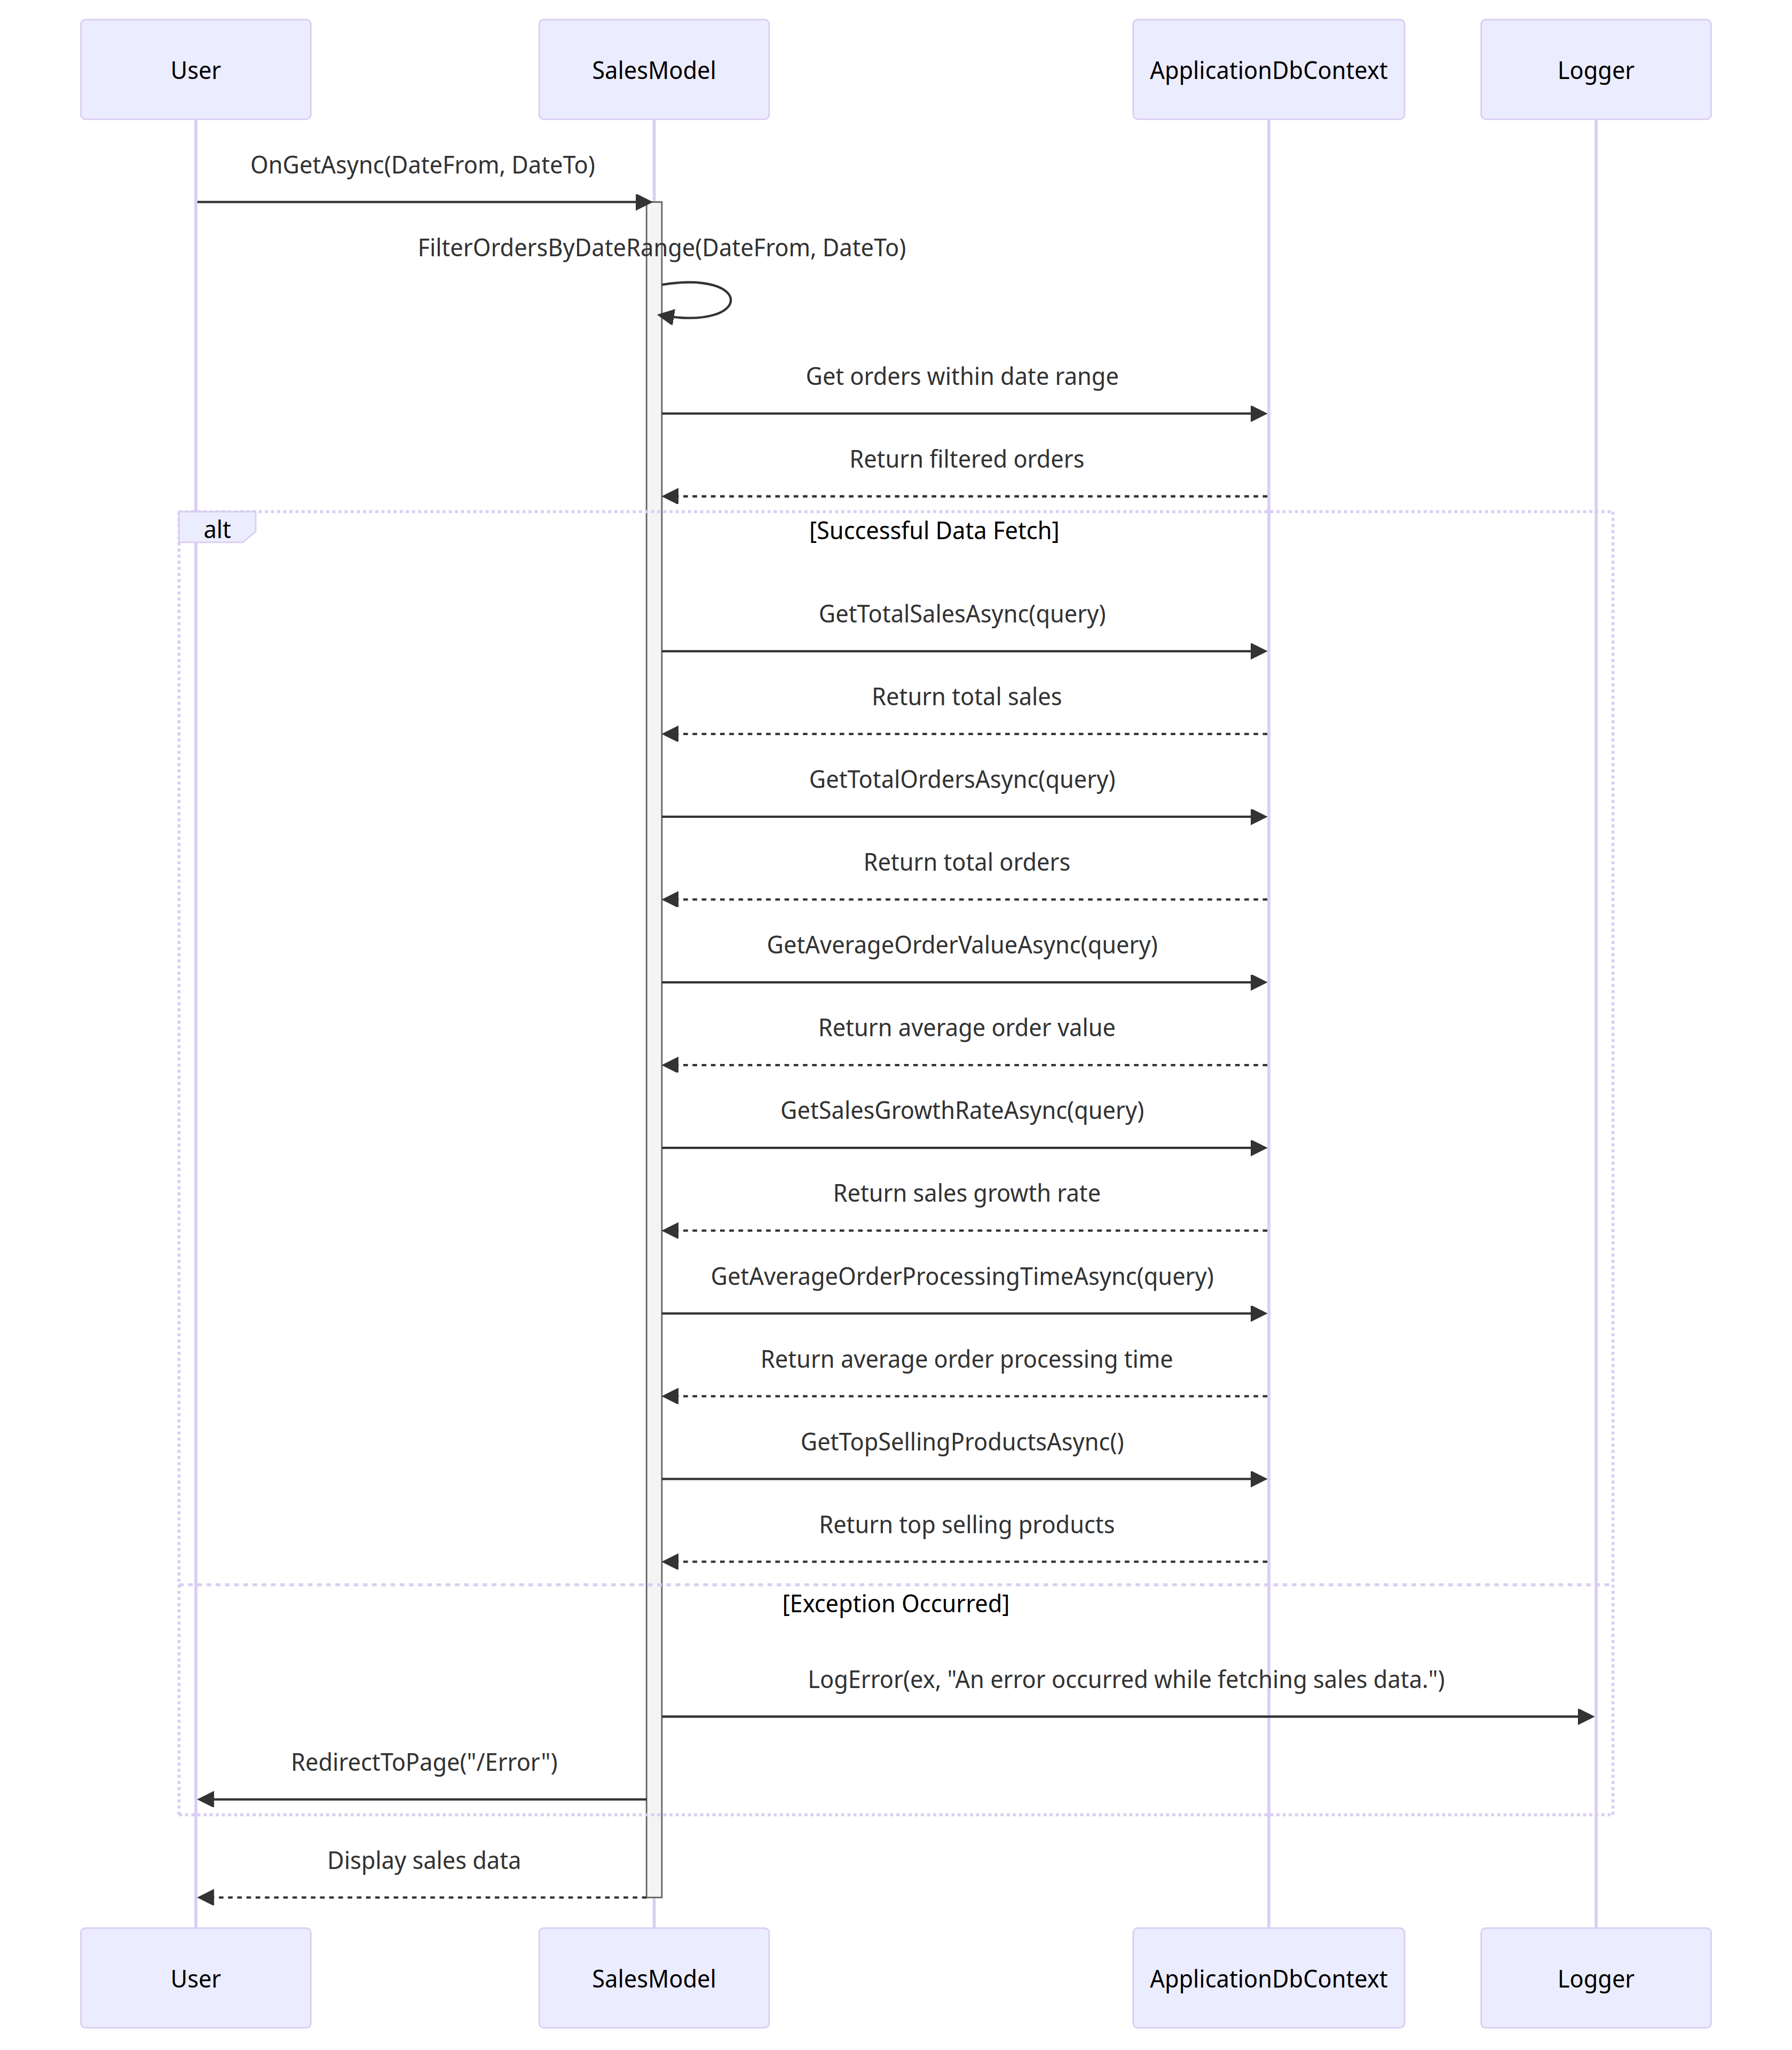
\includegraphics[width=1\textwidth]{figures/diagrams/ssd-ongetasync-salesmodel.png}
    \caption{System Sequence Diagram - OnGetAsync SalesModel}
    \label{fig:ssd-ongetasync-salesmodel}
\end{figure}
\chapter{Kildekode}
\label{appendix:sourcecode}

\section{Modeller}

\subsection{Bruger relaterede modeller}
\label{subsection:user-model}

\inputminted{csharp}{codefiles/models/ApplicationUser.cs}
\label{minted:application-user}

\inputminted{csharp}{codefiles/models/Customer.cs}
\label{minted:customer}

\inputminted{csharp}{codefiles/models/Employee.cs}
\label{minted:employee}

\inputminted{csharp}{codefiles/models/Guest.cs}
\label{minted:guest}

\inputminted{csharp}{codefiles/models/Address.cs}
\label{minted:address}

\inputminted{csharp}{codefiles/models/Company.cs}
\label{minted:company}

\subsection{Merkantilt relaterede modeller}
\label{appendix:mercantile-model}

\inputminted{csharp}{codefiles/models/Product.cs}
\label{minted:product}

\inputminted{csharp}{codefiles/models/Tag.cs}
\label{minted:tag}

\inputminted{csharp}{codefiles/models/Order.cs}
\label{minted:order}

\inputminted{csharp}{codefiles/models/OrderItem.cs}
\label{minted:order-item}

\inputminted{csharp}{codefiles/models/SpecialOrderInstruction.cs}
\label{minted:special-order-instruction}

\inputminted{csharp}{codefiles/models/Basket.cs}
\label{minted:basket}

\inputminted{csharp}{codefiles/models/BasketItem.cs}
\label{minted:basket-item}

\inputminted{csharp}{codefiles/models/BasketActivity.cs}
\label{minted:basketactivity}

\section{Scripts}

\subsection{GitHub scripts}
\label{appendix:github-scripts}
\begin{figure}
    \inputminted{yaml}{codefiles/build.yml}
    \caption{\emph{GitHub Workflows Build}}
    \label{minted:build-yml}
\end{figure}
\chapter{Anvendte Teknologier}
\label{appendix:anvendte-teknologier}
Dette appendix beskriver de frameworks og libraries, der er blevet anvendt i projektet. Hver sektion beskriver kort, hvad hvert framework eller library er, og hvordan det er blevet brugt i projektet.

\section{Overordnede Teknologier}
\subsection{C\#}
C\# (version 8.0.5) er et programmeringssprog udviklet af Microsoft. Sproget er bygget til at være objektorienteret og type-sikkert. C\# er gennemgående anvendt i projektet til håndtering af alt fra databasestyring til routing til \emph{business logic}. Sproget er designet til at være enkelt, sikkert og effektivt, med funktioner som typekontrol, undtagelseshåndtering, hukommelsesstyring og sikkerhedskontrol. Disse funktioner er med til at forhindre almindelige programmeringsfejl og sikkerhedstrusler.

\subsection{.NET}
.NET (version 12.0) er et open-source framework udviklet af Microsoft. Frameworket er modulært og letvægtigt. .NET, sammen med C\#, er gennemgående anvendt i projektet til håndtering af alt fra databasestyring til routing til \emph{business logic}.

\subsection{ASP.NET Core}
ASP.NET Core er et open-source framework, som inkluderer følgende funktioner:
\begin{itemize}
\item \textbf{Modulær}: ASP.NET Core er et modulært framework, der muliggør inkludering af kun nødvendige komponenter i applikationen, hvilket gør den mindre og mere effektiv.
\item \textbf{Cross-platform}: ASP.NET Core kører på Windows, macOS og Linux, hvilket muliggør udvikling og distribution af applikationer på enhver platform.
\item \textbf{Høj ydeevne}: ASP.NET Core er designet til høj ydeevne og effektivitet, og inkluderer funktioner som native understøttelse af asynkron programmering, \emph{Dependency Injection} og middleware for at forbedre ydeevnen.
\item \textbf{Open-source}: ASP.NET Core udvikles og vedligeholdes primært af Microsoft.
\item \textbf{Internetforbundet}: ASP.NET Core fungerer godt med moderne webteknologier som \emph{WebSockets}, \emph{SignalR} og \emph{gRPC}. Realtids og interaktive webapplikationer kan bygges med ASP.NET Core, selvom \emph{Blazor} ofte vil være mere egnet end \emph{Razor Pages}.
\end{itemize}
Store dele af projektet bygger på ASP.NET Core, herunder \emph{Razor Pages} og \emph{Entity Framework Core}.

\subsection{Razor Pages}
\emph{Razor Pages} (RP) er en funktion i ASP.NET Core, der gør kodning af sidefokuserede scenarier lettere og mere produktivt. Frameworket muliggør opbygning af sidefokuserede webapplikationer ved hjælp af en sidebaseret programmeringsmodel. Opsætningen ligner ASP.NET Web Forms, idet hver side har en .cshtml-fil, der indeholder både HTML-markup og C\#-koden, der driver siden. RP er også lig ASP.NET MVC, da de begge bruger Razor-visningsmotoren til at gengive HTML-markup. RP er ideel til små til mellemstore webapplikationer, der primært fokuserer på at vise og indsamle data. RP har derfor været et godt valg til dette projekt.

\subsection{Entity Framework Core}
\emph{Entity Framework Core} (EFC) er en letvægts, udvidelig, open-source og cross-platform version af Entity Framework dataadgangsteknologi. Det fungerer som en objekt-relationsmæssig mapper (\emph{ORM}), der gør det muligt for .NET-udviklere at arbejde med en database ved hjælp af .NET-objekter. EFC eliminerer behovet for det meste af dataadgangskoden, som udviklere normalt skal skrive. EFC understøtter mange database-motorer, herunder SQL Server, MySQL, SQLite, PostgreSQL og andre. EFC kan generere database-tabeller fra kode og generere kode fra database-tabeller. EFC er designet til at fungere med .NET Core-applikationer, men kan også fungere med .NET Framework-applikationer.
EFC inkluderer følgende funktioner:
\begin{itemize}
\item \textbf{Databaseudbydere}: Understøtter mange database-motorer, herunder SQL Server, MySQL, SQLite, PostgreSQL og andre. Den samme kode kan anvendes til at arbejde med forskellige database-motorer.
\item \textbf{Modellering}: Muliggør definition af database-skema ved hjælp af C\#-klasser. Enheder, relationer og begrænsninger kan defineres ved hjælp af attributter eller \emph{Fluent API}.
\item \textbf{Forespørgsler}: Muliggør forespørgsler til databasen ved hjælp af \emph{LINQ} (\emph{Language Integrated Query}). LINQ-forespørgsler kan skrives i C\#-kode, og EFC oversætter dem til SQL-forespørgsler.
\item \textbf{Lagring af data}: Muliggør datalagring i databasen ved hjælp af \emph{DbContext}-klassen. Enheder kan tilføjes, opdateres og slettes, og EFC genererer de nødvendige SQL-kommandoer.
\item \textbf{Ændringssporing}: EFC sporer ændringer i enheder og genererer nødvendige SQL-kommandoer for at persistere ændringer i databasen.
\item \textbf{Migrationer}: Muliggør oprettelse og anvendelse af database-migrationer, der bruges til at opdatere database-skemaet, når applikationen udvikler sig.
\item \textbf{Transaktioner}: Understøtter transaktioner, der muliggør gruppering af flere databaseoperationer i en enkelt enhed af arbejde.
\item \textbf{Samtidighed}: Understøtter \emph{optimistic concurrency}, der muliggør, at flere brugere kan arbejde med de samme data uden konflikter.
\item \textbf{Ydelse}: EFC er designet til høj ydeevne og effektivitet. Inkluderer funktioner som forespørgselscache, kompilerede forespørgsler og batchopdateringer for at forbedre ydeevnen.
\end{itemize}

\subsubsection{Bootstrap}
\emph{Bootstrap} (version 5.3.3) er et open-source CSS framework udviklet af Twitter. Frameworket er letvægtigt og nemt at anvende. Bootstrap er blevet brugt til frontend-udvikling i projektet og har håndteret alt fra styling til responsivt design.

\subsection{JavaScript}
\emph{JavaScript} (version ES6) er et programmeringssprog udviklet af Netscape. Sproget er letvægtigt og nemt at bruge. JavaScript er blevet anvendt til frontend-udvikling i projektet og har håndteret alt fra DOM-manipulation til event handling. Dette inkluderer brug af \emph{Chart.js}, som anvendes på forsiden med billedekarusellen.

\subsection{Font Awesome}
\emph{Font Awesome} er et open-source ikon library udviklet af Dave Gandy. Libraryet er letvægtigt og nemt at anvende. Font Awesome er blevet brugt til frontend-udvikling i projektet for at implementere ikoner til heuristisk UI/UX.

\subsection{Chart.js}
\emph{Chart.js} (version 4.4.1) er et open-source chart library udviklet af Nick Downie. Libraryet er letvægtigt og nemt at anvende. Chart.js er blevet anvendt til frontend-udvikling i projektet og har håndteret datavisualisering i Admin/Analytics.

\subsection{SQL}
\emph{SQL} (\emph{Structured Query Language}) er et programmeringssprog udviklet til håndtering af relationelle databaser. Selvom \emph{LINQ} har været den primære metode til interaktion med databasen, er SQL blevet brugt som udgangspunkt og senere oversat til LINQ. Microsofts udgave af SQL, kaldet \emph{T-SQL}, er blevet anvendt i projektet og delvist håndteret med \emph{MS SQL Server Management Studio} (v 19.3). SSMS har blandt andet været brugt til at oprette .bak-filer, der er blevet brugt til at oprette databasen på simply.com.

\section{C\# Specifikke Teknologier}
Denne sektion beskriver de frameworks og libraries, der er blevet anvendt i projektet, og som er specifikke for C\#. Informationen er primært fra Microsofts dokumentation og er blevet tilpasset projektet. 
Hvor det har været muligt, er strukturen opsat efter \textbf{enkelthed}, \textbf{klarhed}, \textbf{sikkerhed} og \textbf{ydelse}. 

\subsection{ASP.NET Core Identity}
ASP.NET Core Identity er et medlemssystem, der tilføjer loginfunktionalitet til ASP.NET Core-applikationer. Brugere kan oprette en konto, logge ind og logge ud. ASP.NET Core Identity inkluderer følgende funktioner:
\begin{itemize}
\item Lagrer brugeroplysninger i en SQL Server-database ved hjælp af EFC.
\item Tilbyder et standard-UI til login, registrering og håndtering af brugerprofil.
\item Tilbyder funktionalitet til konto-bekræftelse og nulstilling af adgangskode.
\item Aktiverer konto-låsning for at beskytte mod \emph{brute force}-angreb.
\item Aktiverer tofaktor-autentificering ved hjælp af SMS eller e-mail.
\item Tilbyder cookie-autentificering som standardautentificeringsmetode.
\item Tillader tilpasning af tokenudbyderen og e-mail-senderen.
\item Tillader tilpasning af brugerprofilen ved at tilføje brugerdefinerede egenskaber.
\item Tillader tilpasning af UI'en ved at ændre Razor-visningerne.
\item Tilbyder en \emph{UserManager}-klasse til at arbejde med brugere.
\end{itemize}
ASP.NET Core IdentityUser er brugerklassen til ASP.NET Core Identity. Den indeholder egenskaber som Id, UserName, Email osv., der er fælles for de fleste brugerklasser. IdentityUser kan udvides for at tilføje brugerdefinerede egenskaber. Dette er gjort på følgende måde:
\begin{enumerate}
\item \textbf{ApplicationUser.cs}: Denne klasse arver fra IdentityUser-klassen, som leveres af ASP.NET Core Identity. Dette betyder, at ApplicationUser arver alle egenskaber fra IdentityUser (som Id, UserName, Email osv.) og kan også tilføje yderligere egenskaber. I dette tilfælde er FirstName, LastName og Address tilføjet.
\item \textbf{Customer.cs og Employee.cs}: Disse klasser arver fra ApplicationUser, hvilket betyder, at de arver alle egenskaber fra ApplicationUser og dermed IdentityUser. De tilføjer også deres egne specifikke egenskaber. Dette er en almindelig måde at udvide brugermodellen i ASP.NET Core Identity for at inkludere yderligere data, der er specifikke for applikationen.
\item \textbf{ApplicationDbContext.cs}: Denne klasse arver fra IdentityDbContext, som er en DbContext, der er specifikt designet til at arbejde med ASP.NET Core Identity. Den inkluderer DbSet-egenskaber for Customer og Employee, hvilket betyder, at disse typer brugere vil blive inkluderet i databasekonteksten.
\item \textbf{Program.cs}: Den valgte kode i denne fil konfigurerer ASP.NET Core Identity-systemet. Den tilføjer det standardidentitetssystem med ApplicationUser som brugertype og ApplicationDbContext som kontekst. Den tilføjer også identitetskernen for Customer og Employee-typer, hvilket betyder, at disse typer brugere vil blive inkluderet i identitetssystemet.
\end{enumerate}

\subsection{Fluent API}
\emph{Fluent API} er et open-source framework udviklet af Microsoft, der bruges til databasestyring i projektet. Det håndterer alt fra oprettelse af databaser til CRUD-operationer.  \emph{Fluent API} inkluderer følgende funktioner:
\begin{itemize}
\item \textbf{Enkelhed}: \emph{Fluent API} gør det nemt at definere og konfigurere database-skemaer ved hjælp af C\#-kode, hvilket eliminerer behovet for at bruge konventioner eller dataannotations.
\item \textbf{Klarhed}: \emph{Fluent API} giver en tydelig og udtryksfuld måde at specificere databasens konfigurationer på, hvilket gør koden lettere at læse og vedligeholde.
\item \textbf{Sikkerhed}: \emph{Fluent API} kan hjælpe med at sikre, at database-skemaet er korrekt konfigureret ved at centralisere konfigurationslogik og gøre det lettere at validere opsætningen.
\item \textbf{Ydelse}: \emph{Fluent API} er designet til at være effektiv ved at give mulighed for præcis kontrol over databasekonfigurationer, hvilket kan forbedre databaseydelsen og reducere risikoen for fejl.
\end{itemize}
\emph{Fluent API} er blevet anvendt til at konfigurere database-skemaer i projektet. Dette kan ses i mappen \emph{/Config/.cs}, hvor der er konfigureret forhold mellem forskellige entiteter.

\subsection{LINQ}
\emph{LINQ} (\emph{Language Integrated Query}) er et open-source framework udviklet af Microsoft, som håndterer databasestyring i webapplikationer. LINQ er blevet anvendt til at håndtere databasestyring i projektet, herunder forespørgsler og CRUD-operationer. LINQ muliggør skrivning af SQL-lignende forespørgsler i C\#. Det er en kraftfuld funktion, der kan hjælpe med at skrive mere effektiv kode i projektet.
LINQ inkluderer følgende funktioner:
\begin{itemize}
\item \textbf{Enkelhed}: LINQ gør det nemt at skrive SQL-lignende forespørgsler i C\# ved at inkludere forespørgselslogik direkte i koden.
\item \textbf{Klarhed}: LINQ gør det nemt at se, hvordan forespørgsler er struktureret, da det eliminerer behovet for at skrive komplekse SQL-forespørgsler.
\item \textbf{Sikkerhed}: LINQ gør det nemt at validere forespørgsler, da det eliminerer behovet for at skrive kompleks valideringslogik.
\item \textbf{Ydelse}: LINQ er designet til høj ydeevne og effektivitet, da det eliminerer behovet for at skrive, og derefter suboptimere, komplekse SQL-forespørgsler.
\end{itemize}

\subsection{HttpContextAccessor}
\emph{HttpContextAccessor} er en klasse i ASP.NET Core, der giver adgang til HTTP anmodningsoplysninger i applikationen. Det muliggør adgang til HTTP anmodningsoplysninger, såsom URL, metode, hoveder og cookies, fra enhver del af applikationen.
\begin{itemize}
\item \textbf{Enkelhed}: \emph{HttpContextAccessor} gør det nemt at få adgang til HTTP anmodningsoplysninger i hele applikationen, uden at skulle videresende disse oplysninger gennem forskellige lag af applikationen.
\item \textbf{Klarhed}: \emph{HttpContextAccessor} giver en klar og direkte måde at tilgå HTTP-anmodningsoplysninger på, hvilket gør koden lettere at læse og forstå.
\item \textbf{Sikkerhed}: \emph{HttpContextAccessor} kan hjælpe med at validere og sikre HTTP-anmodningsoplysninger ved at centralisere adgangen til disse data, hvilket kan reducere risikoen for fejl og sikkerhedsproblemer.
\item \textbf{Ydelse}: \emph{HttpContextAccessor} er designet til at være effektiv ved at give hurtig adgang til nødvendige HTTP-anmodningsoplysninger uden behov for kompleks kode til at hente disse data.
\end{itemize}

\subsubsection{Primary Constructors}
I dette projekt er \emph{Primary Constructors} anvendt, som er en funktion i C\# 10.0. Primary Constructors giver mulighed for at definere en primær konstruktør direkte i klassens definition, i stedet for at bruge en separat konstruktørmetode. Dette gør det nemmere at definere og initialisere objekter i C\#. Primary Constructors inkluderer følgende funktioner:
\begin{itemize}
\item \textbf{Enkelhed}: Primary Constructors gør det nemt at definere og initialisere objekter i C\# ved at inkludere konstruktørlogik direkte i klassens definition.
\item \textbf{Klarhed}: Primary Constructors gør det nemt at se, hvordan objekter initialiseres, da konstruktørlogikken er synlig i klassens definition.
\item \textbf{Sikkerhed}: Primary Constructors gør det nemt at validere objekter, da konstruktørlogikken kan inkludere valideringslogik.
\item \textbf{Ydelse}: Primary Constructors er designet til høj ydeevne og effektivitet, da de eliminerer behovet for at kalde en separat konstruktørmetode.
\end{itemize}
Primary Constructors er oplagt til \emph{PageModels}, hvor der kan være behov for at lave \emph{Dependency Injection}. Dette er gjort i dette projekt, hvor Primary Constructors er blevet anvendt til at initialisere de fleste PageModels.

\subsubsection{Nullable Reference Types}
I dette projekt er \emph{Nullable Reference Types} anvendt, som er en funktion i C\# 8.0. Nullable Reference Types inkluderer følgende funktioner:
\begin{itemize}
\item \textbf{Enkelhed}: Nullable Reference Types gør det nemt at angive, om en reference kan være null i C\# ved at inkludere nullabilitylogik direkte i koden.
\item \textbf{Klarhed}: Nullable Reference Types gør det nemt at se, om en reference kan være null, da nullabilitylogikken er synlig i koden.
\item \textbf{Sikkerhed}: Nullable Reference Types gør det nemt at validere, om en reference kan være null, da nullabilitylogikken kan inkludere valideringslogik.
\item \textbf{Ydelse}: Nullable Reference Types er designet til høj ydeevne og effektivitet, da det eliminerer behovet for at skrive komplekse null-checks.
\end{itemize}
Nullable Reference Types giver mulighed for at angive, om en reference kan være null i C\#. Nullable Reference Types er en kraftfuld funktion, der kan give en mere sikker og robust kode. Dette er gjort i dette projekt, hvor Nullable Reference Types er blevet anvendt til at angive, om en reference kan være null.
Dette ses især i modelklasser, hvor der er behov for at angive, om en reference kan være null. så fx. et objekt kan instansieres uden at have en værdi.

\subsubsection{Top-level Statements}
I dette projekt er \emph{Top-level Statements} anvendt, som er en funktion i C\# 9.0. Top-level Statements giver mulighed for at skrive kode uden at skulle definere en klasse eller en metode. Top-level Statements inkluderer følgende funktioner:
\begin{itemize}
\item \textbf{Enkelhed}: Top-level Statements gør det nemt at skrive kode uden at skulle definere en klasse eller en metode i C\#.
\item \textbf{Klarhed}: Top-level Statements gør det nemt at se, hvordan kode er struktureret, da det eliminerer behovet for at skrive unødvendig boilerplate-kode.
\item \textbf{Sikkerhed}: Top-level Statements gør det nemt at validere kode, da det eliminerer behovet for at skrive komplekse strukturer.
\item \textbf{Ydelse}: Top-level Statements er designet til høj ydeevne og effektivitet, da de eliminerer behovet for at skrive unødvendig boilerplate-kode.
\end{itemize}

\subsubsection{Async/Await}
I dette projekt er \emph{Async/Await} anvendt, som er en funktion i C\# 5.0. Async/Await giver mulighed for at skrive asynkron kode i C\#. Async/Await inkluderer følgende funktioner:
\begin{itemize}
\item \textbf{Enkelhed}: Async/Await gør det nemt at skrive asynkron kode i C\# ved at inkludere asynkron logik direkte i koden.
\item \textbf{Klarhed}: Async/Await gør det nemt at se, hvordan asynkron kode er struktureret, da det eliminerer behovet for at skrive komplekse callback-funktioner.
\item \textbf{Sikkerhed}: Async/Await gør det nemt at validere asynkron kode, da det eliminerer behovet for at skrive komplekse fejlhåndteringslogik.
\item \textbf{Ydelse}: Async/Await er designet til høj ydeevne og effektivitet, da det eliminerer behovet for at skrive komplekse callback-funktioner.
\end{itemize}

\subsubsection{LINQ}
I dette projekt er \emph{LINQ} anvendt, som er en funktion i C\# 3.0. LINQ muliggør skrivning af SQL-lignende forespørgsler i C\#. LINQ er en kraftfuld funktion, der kan hjælpe med at skrive mere effektiv og udtryksfuld kode. LINQ inkluderer følgende funktioner:
\begin{itemize}
\item \textbf{Enkelhed}: LINQ gør det nemt at skrive SQL-lignende forespørgsler i C\# ved at inkludere forespørgselslogik direkte i koden.
\item \textbf{Klarhed}: LINQ gør det nemt at se, hvordan forespørgsler er struktureret, da det eliminerer behovet for at skrive komplekse SQL-forespørgsler.
\item \textbf{Sikkerhed}: LINQ gør det nemt at validere forespørgsler, da det eliminerer behovet for at skrive komplekse valideringslogik.
\item \textbf{Ydelse}: LINQ er designet til høj ydeevne og effektivitet, da det eliminerer behovet for at skrive komplekse SQL-forespørgsler.
\end{itemize}

\subsubsection{Delegates}
I dette projekt er \emph{Delegates} anvendt, som er en funktion i C\# 1.0. Delegates muliggør oprettelse og brug af funktioner som objekter i C\#. Delegates er en kraftfuld funktion, der kan hjælpe med at skrive mere fleksibel og genbrugelig kode. Delegates inkluderer følgende funktioner:
\begin{itemize}
\item \textbf{Enkelhed}: Delegates gør det nemt at oprette og bruge funktioner som objekter i C\# ved at inkludere delegatlogik direkte i koden.
\item \textbf{Klarhed}: Delegates gør det nemt at se, hvordan funktioner er struktureret, da det eliminerer behovet for at skrive komplekse callback-funktioner.
\item \textbf{Sikkerhed}: Delegates gør det nemt at validere funktioner, da det eliminerer behovet for at skrive komplekse valideringslogik.
\item \textbf{Ydelse}: Delegates er designet til høj ydeevne og effektivitet, da det eliminerer behovet for at skrive komplekse callback-funktioner.
\end{itemize}

\subsubsection{Generics}
I dette projekt er \emph{Generics} anvendt, som er en funktion i C\# 2.0. Generics muliggør oprettelse af generiske typer og metoder i C\#. Generics er en kraftfuld funktion, der kan hjælpe med at skrive mere fleksibel og genbrugelig kode. Generics inkluderer følgende funktioner:
\begin{itemize}
\item \textbf{Enkelhed}: Generics gør det nemt at oprette generiske typer og metoder i C\# ved at inkludere generisk logik direkte i koden.
\item \textbf{Klarhed}: Generics gør det nemt at se, hvordan generiske typer og metoder er struktureret, da det eliminerer behovet for at skrive komplekse generiske klasser og metoder.
\item \textbf{Sikkerhed}: Generics gør det nemt at validere generiske typer og metoder, da det eliminerer behovet for at skrive komplekse valideringslogik.
\item \textbf{Ydelse}: Generics er designet til høj ydeevne og effektivitet, da det eliminerer behovet for at skrive komplekse generiske klasser og metoder.
\end{itemize}

\section{Eksterne Teknologier}
\subsection{Smtp4dev}
\emph{Smtp4dev} er en open-source email service udviklet af Rnwood. Servicen håndterer emailafsendelse i webapplikationer. Smtp4dev er blevet brugt til håndtering af emailafsendelse og modtagelse i projektet under udvikling.

\subsection{MimeKit og Mailkit}
\emph{MimeKit} og \emph{MailKit} er open-source email libraries. MimeKit og MailKit er blevet brugt til håndtering af emailafsendelse og modtagelse i projektet, og har håndteret alt fra emailverifikation til emailnotifikationer.
\chapter{Doxygen Dokumentation}
\label{appendix:doxygen}


\includepdf[pages=-, frame=true]{appendix/refman.pdf}

\end{document}